\chapter{离子电流干扰去除分析方法}
\section{电容式离子电流检测电路的局限性}
\par 如下图所示的是1250r/min,2000r/min,3000r/min下在30\%,40\%,50\%时的缸压和离子电流曲线。
\begin{figure}[H]
	\centering
	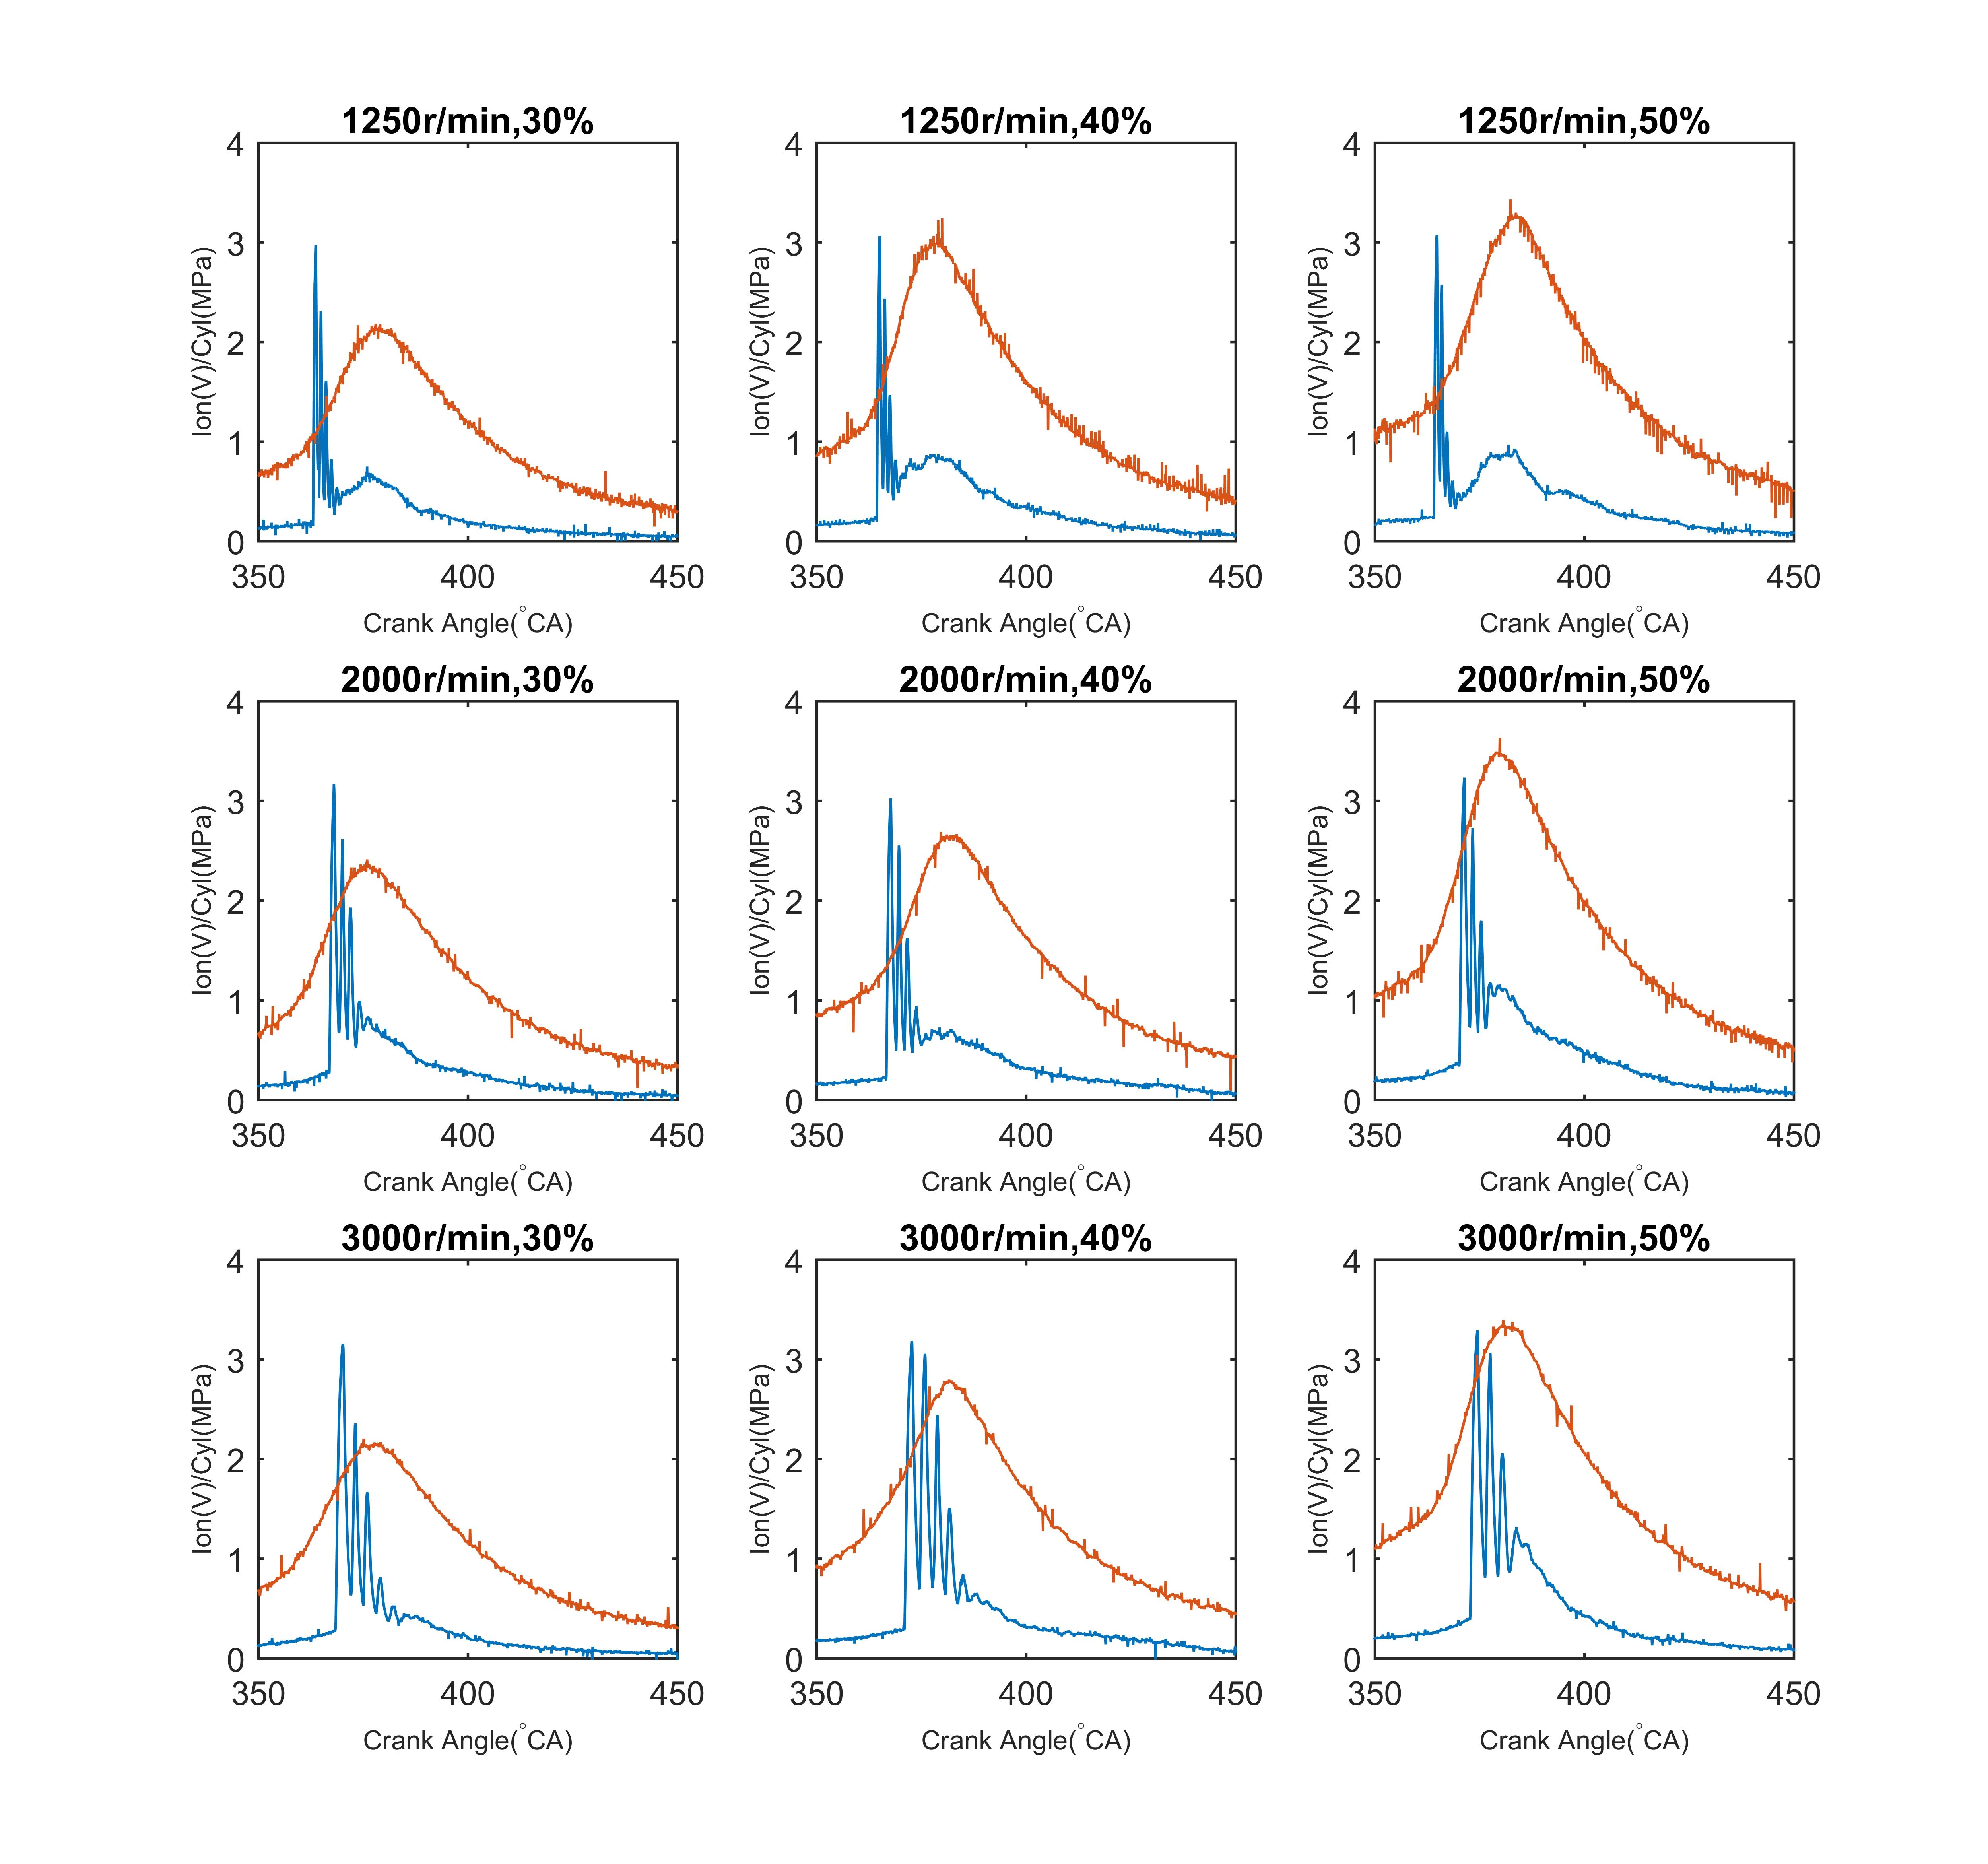
\includegraphics[width=\textwidth]{thesis_figure/ion_chapter/ion_vary_trending}
	\caption{不同转速、不同负荷下的缸压和离子电流}
	\label{fig:ion_cyp}
\end{figure}
从图\ref{fig:ion_cyp}中可以看到从上到下看是同一负荷下,随着转速增加的离子电流曲线;从左向右是同一转速下,随着负荷增大的离子电流曲线。
随着转速的增加,火焰后期的离子电流是逐渐被淹没的。也就是说点火干扰期将离子电流的性质淹没了,无法获得离子电流的特征值。
\subsection{点火放电干扰的来源和性质}
由于点火干扰期将离子电流的性质淹没,因此我们需要了解点火放电干扰的来源及其稳定的性质。如图\ref{fig:itf_rs}所示,通过检测次级电压来和离子电流进行对比可以发现,次级电压
点火放电过程的放电干扰期和离子电流的点火干扰期重合。
\begin{figure}[H]
\begin{minipage}{0.5\linewidth}
	\centering
	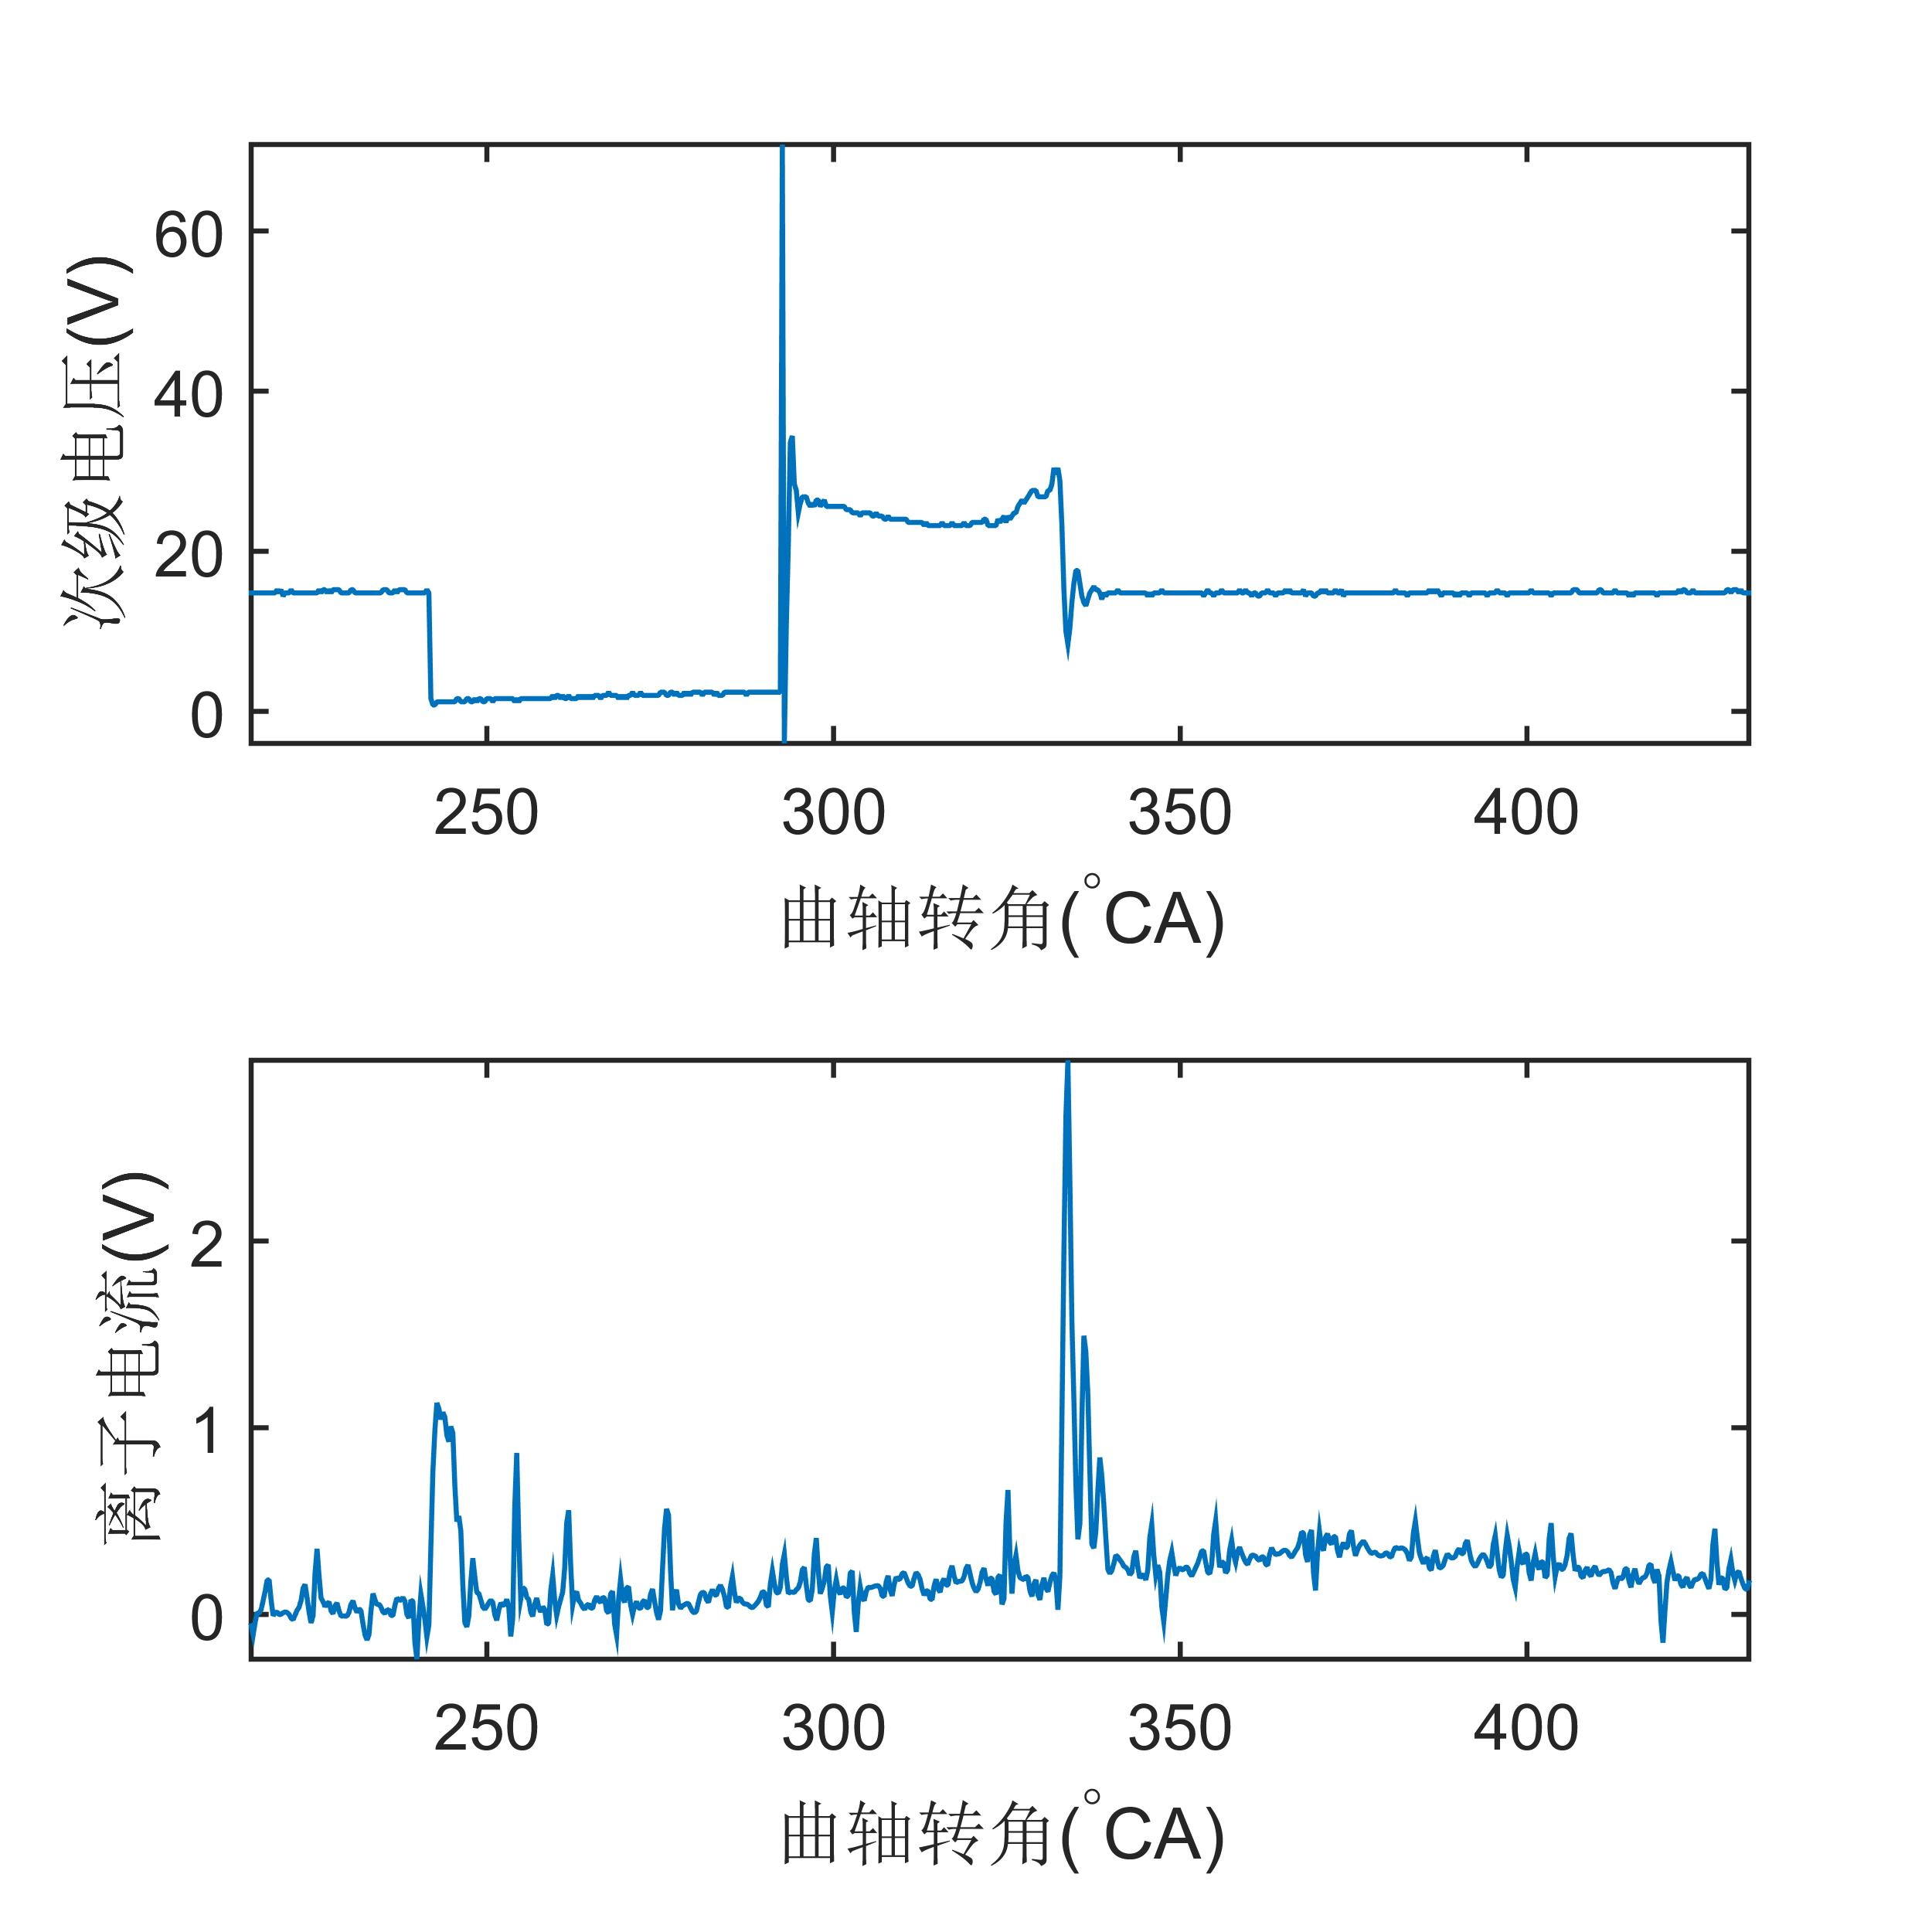
\includegraphics[width = \textwidth]{thesis_figure/ion_chapter/interfere_reason}
\end{minipage}
\begin{minipage}{0.5\linewidth}
	\centering
	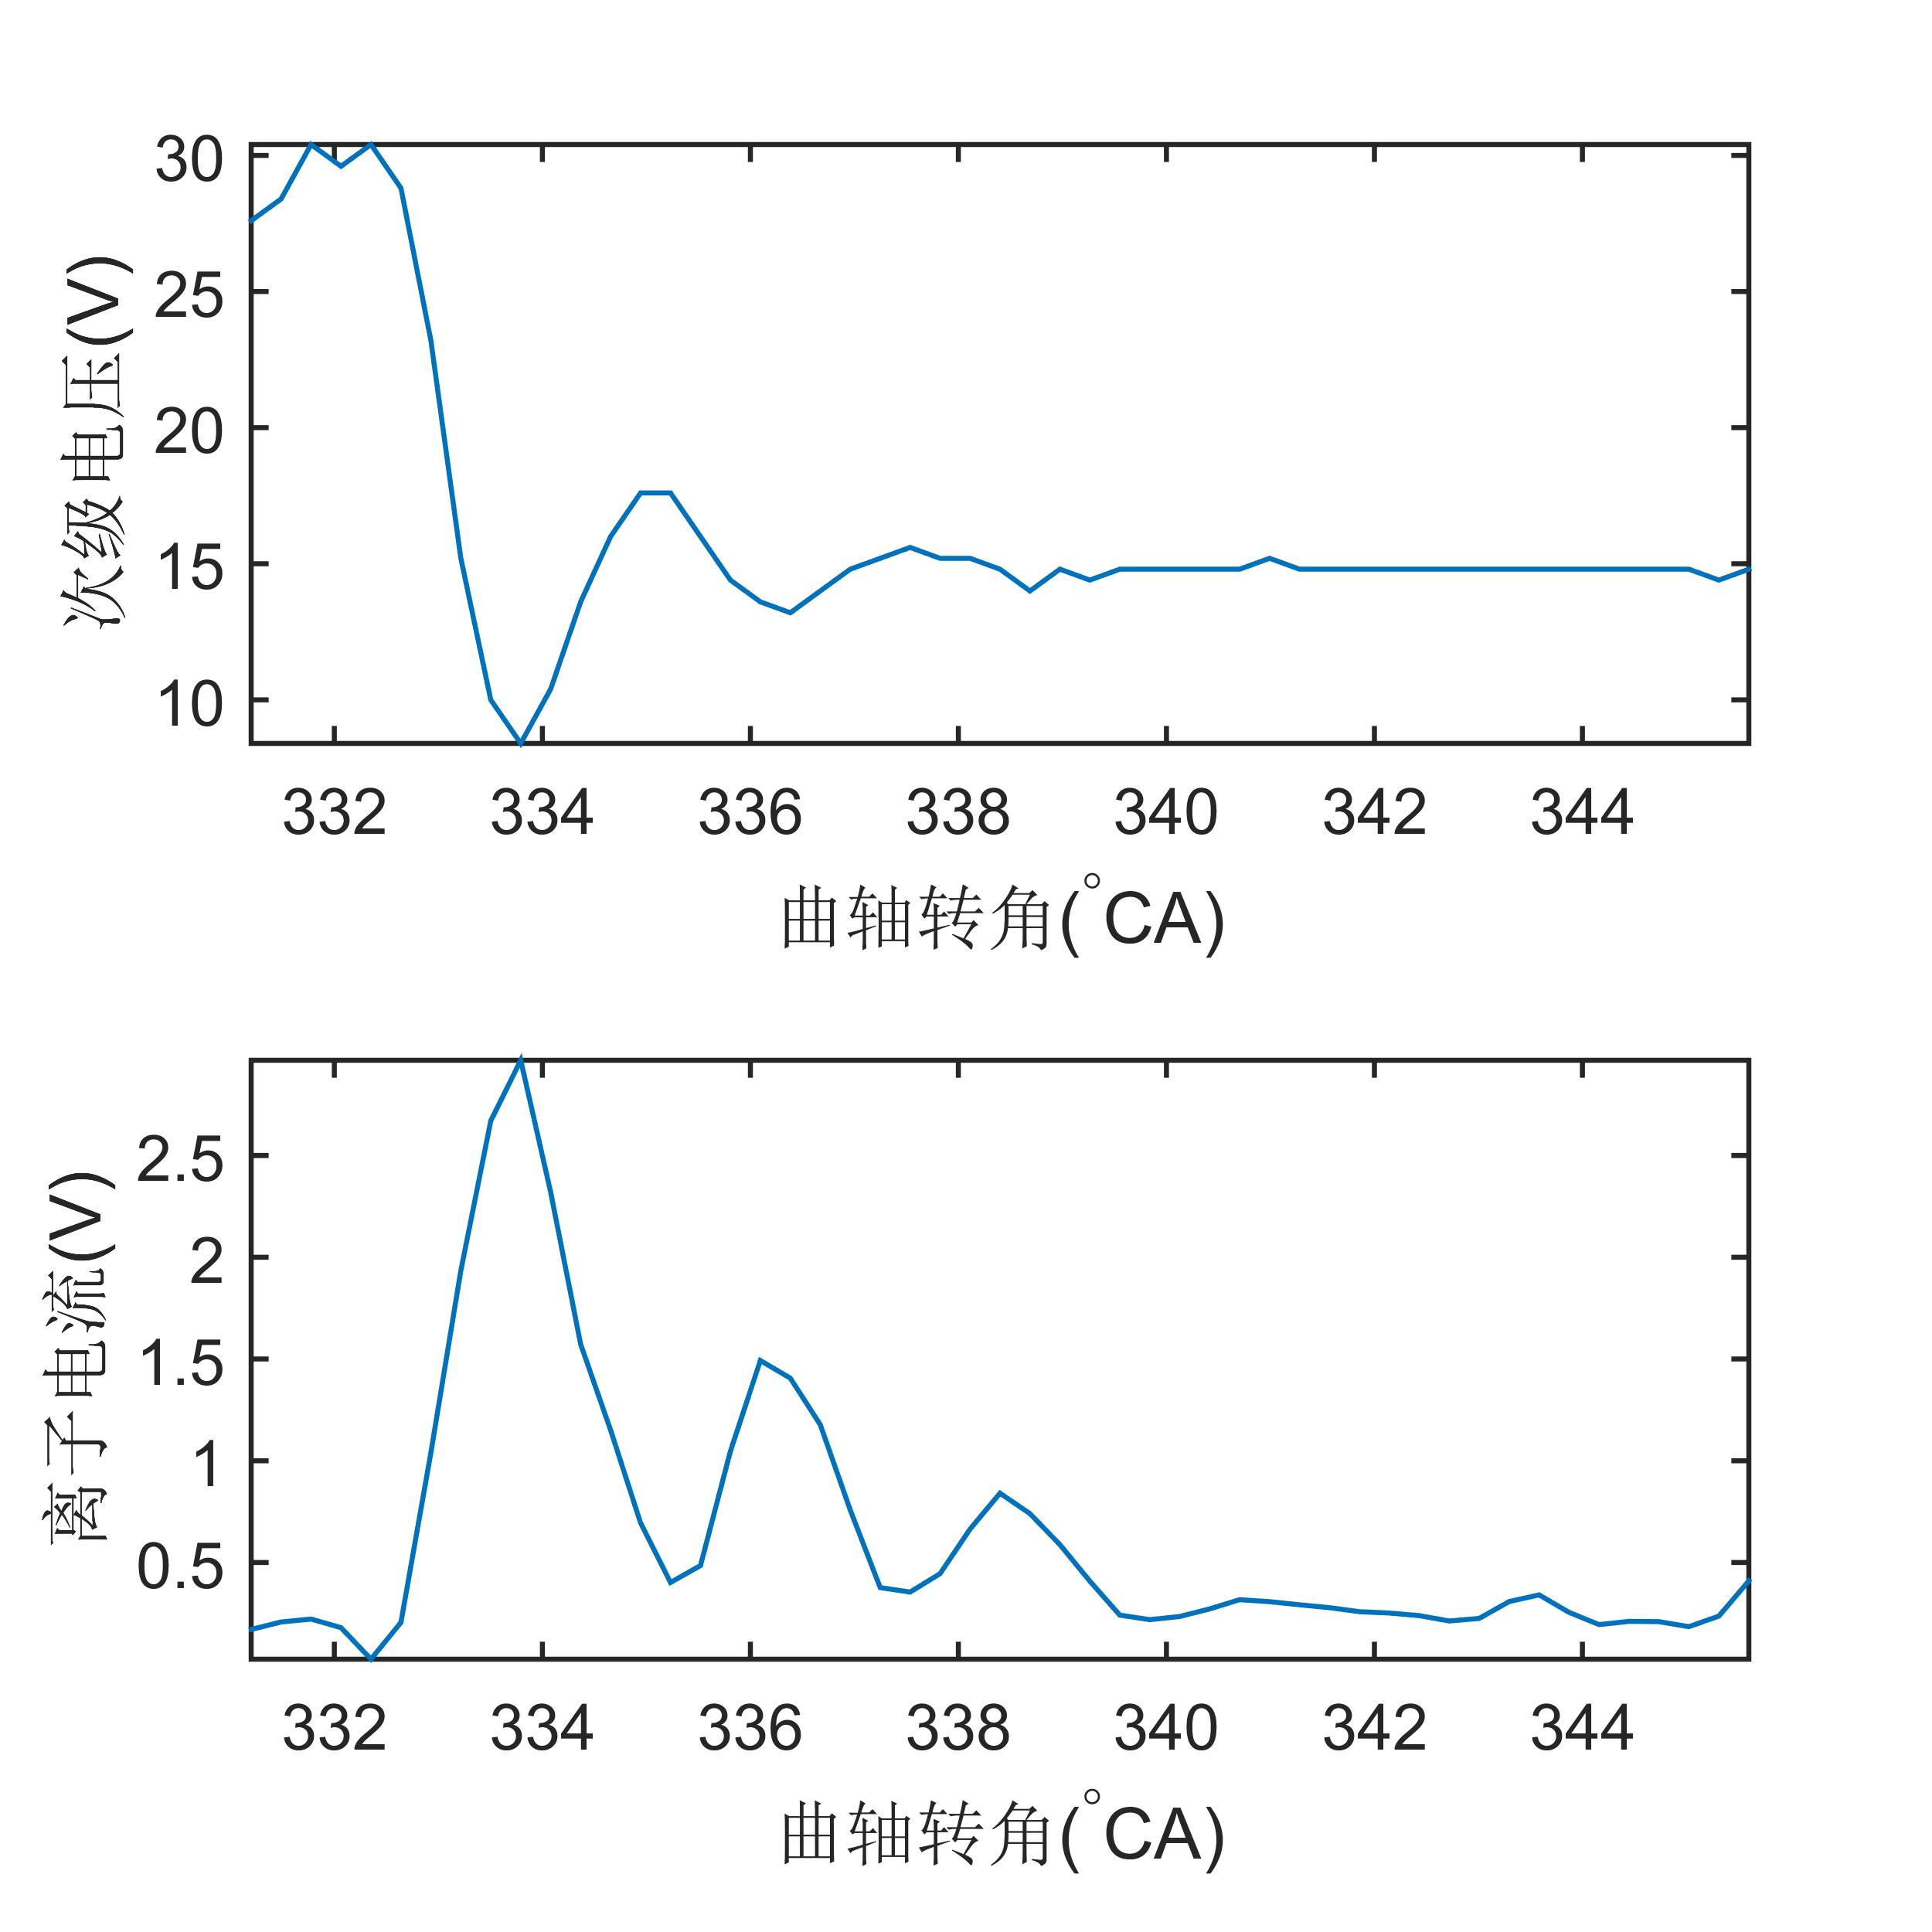
\includegraphics[width = \textwidth]{thesis_figure/ion_chapter/itf_rs}
\end{minipage}
	\caption{次级电压和离子电流对比}
	\label{fig:itf_rs}
\end{figure}
\par 我们将重叠的部分进行放大,可以看到两者的频率也是相同的。
经过计算可以得到该放电周期为$0.12ms$,时长为$1ms$。由以上两张图的分析结果可以知道,离子电流的点火干扰期是由次级线圈的点火放电信号导致的,会产生一个特定频率的震荡信号。我们将不同转速下的离子电流
曲线放在一起比较,可以看到如图\ref{fig:dif_rpm_ion}所示的图形。
\begin{figure}[!ht]
	\centering
	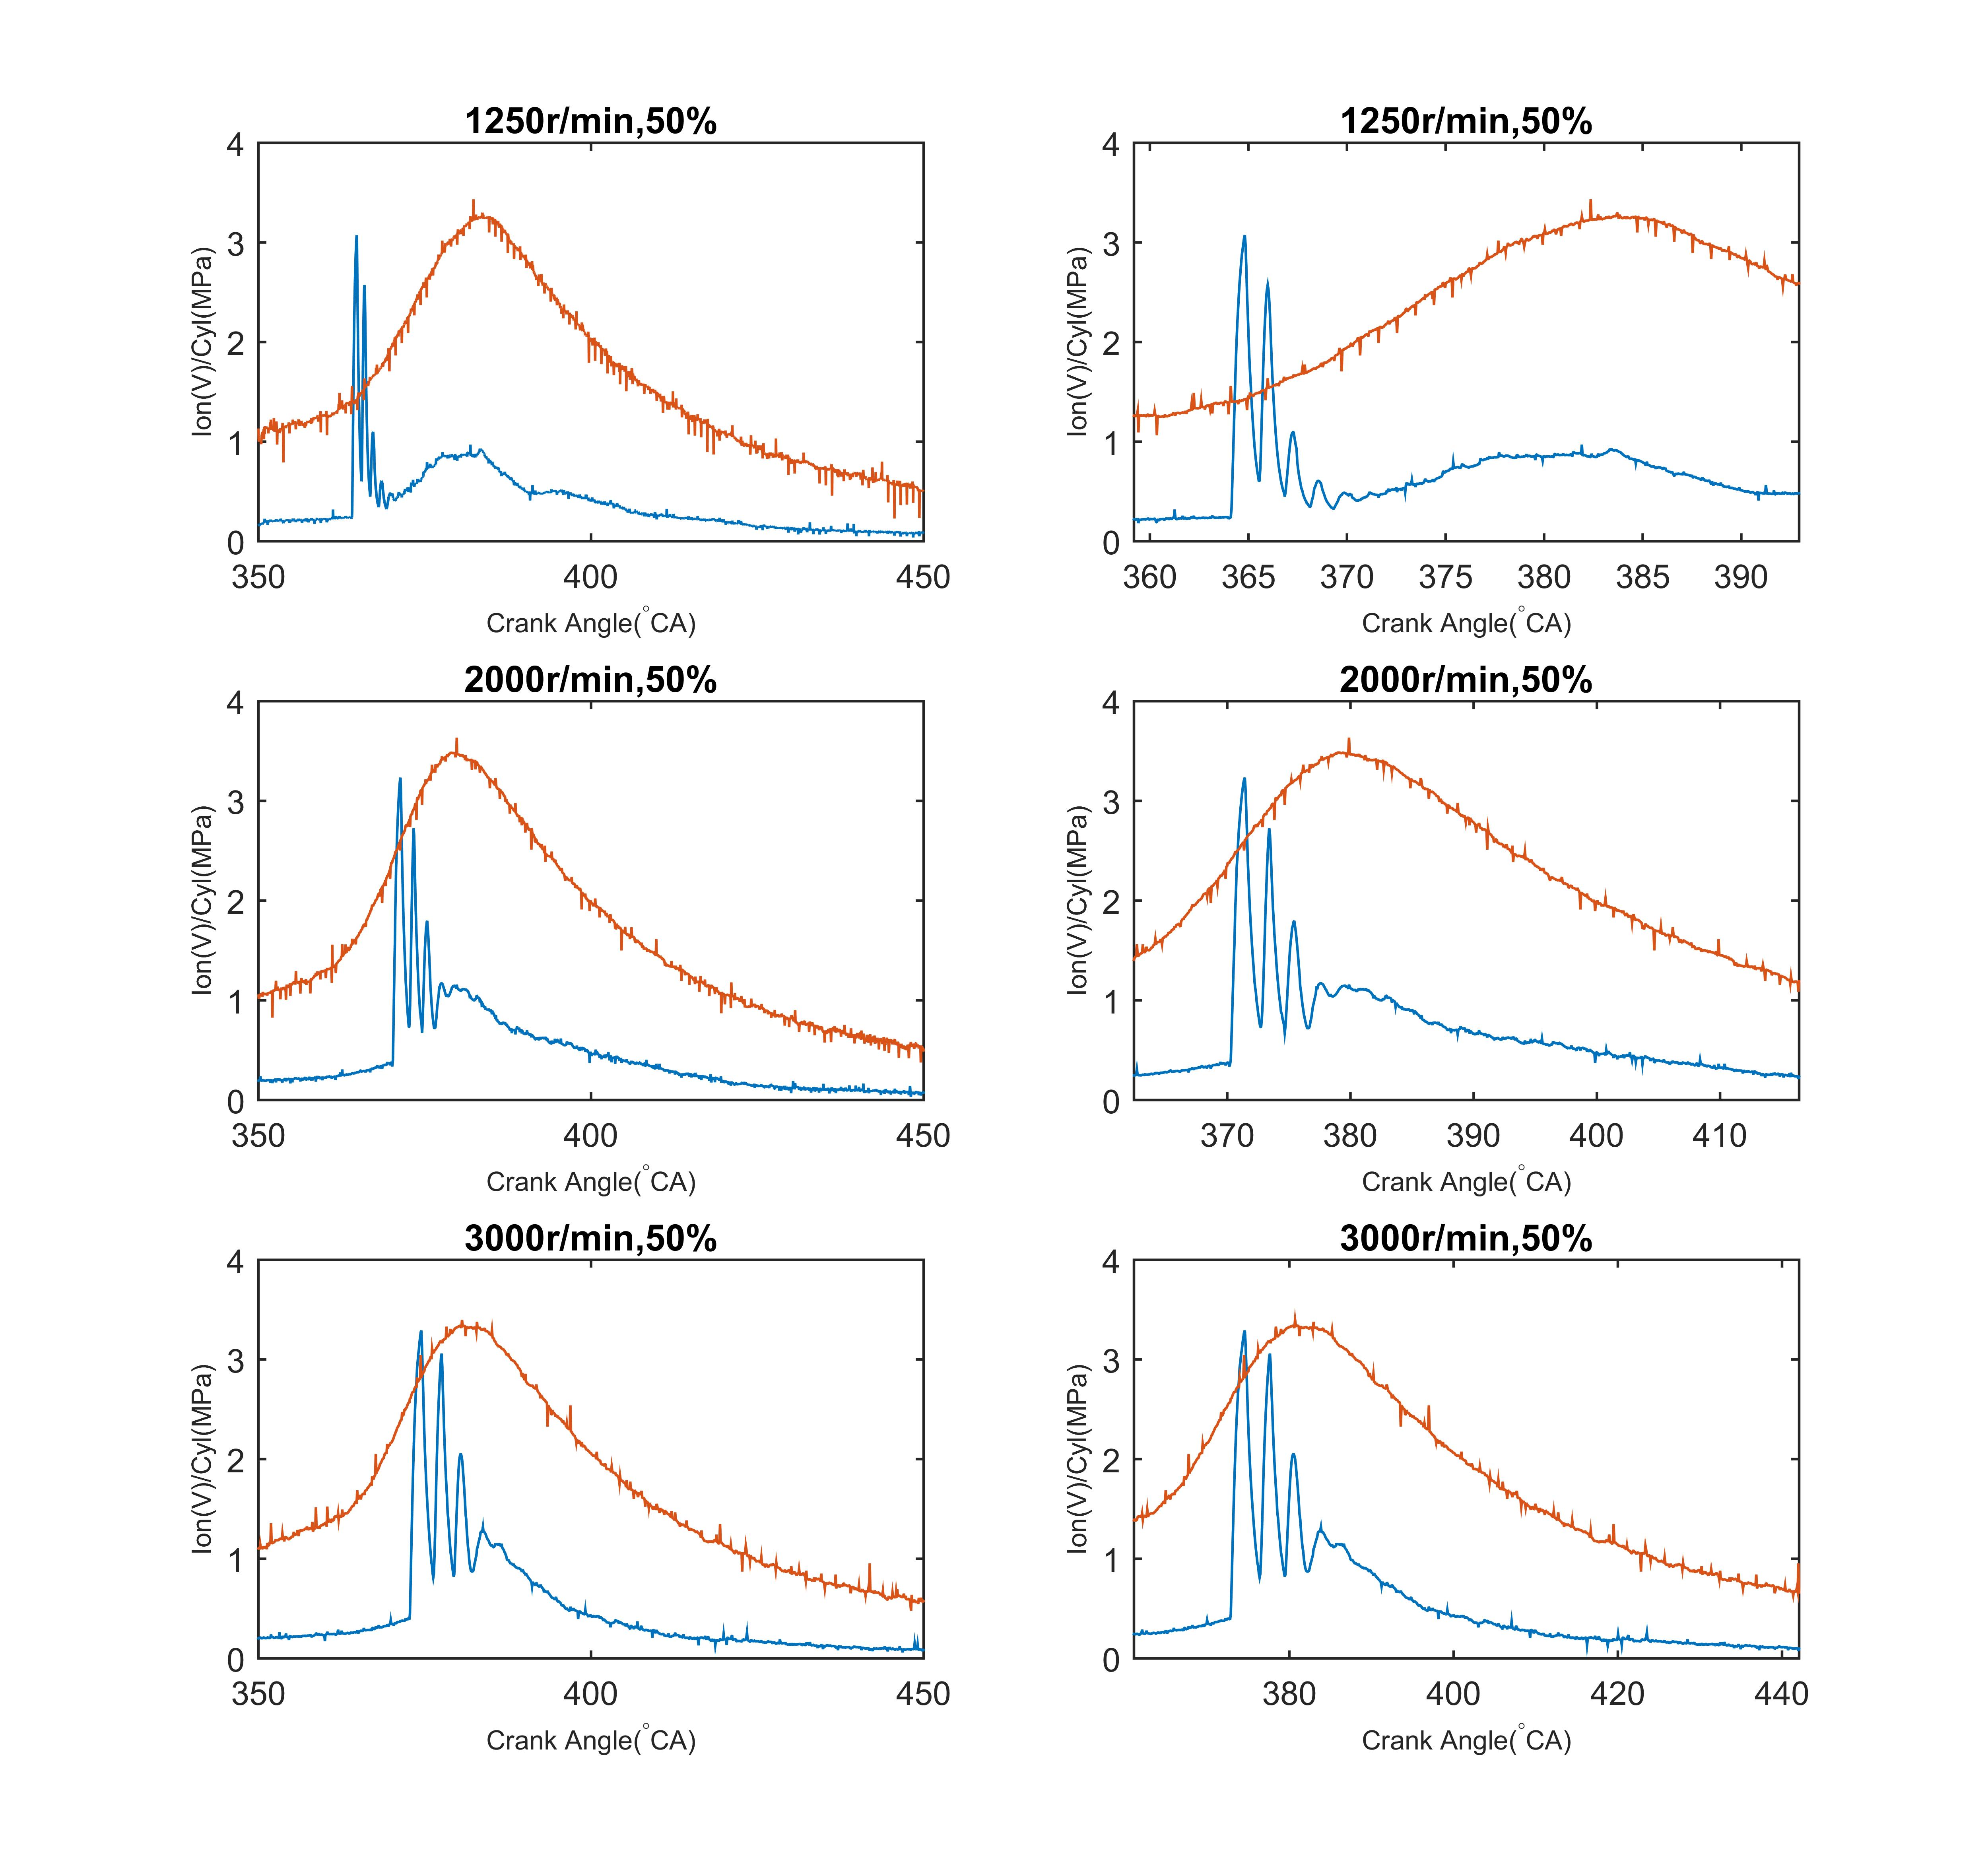
\includegraphics[width=\textwidth]{thesis_figure/ion_chapter/dif_rpm_ion}
	\caption{不同转速下的离子电流按曲轴转角对比和按时间对比}
	\label{fig:dif_rpm_ion}
\end{figure}
\par 左列的三张图从上到下为随着转速增加,离子电流按照曲轴转角进行对比,曲轴转角窗口长度为100度,可以发现点火震荡信号在不断淹没火焰前锋期和火焰后期。右列的三张图从上到下为随着转速增加,
离子电流按时间进行对比,时间窗口长度为5毫秒时间,可以发现震荡信号的频率和长度不变。左右两列曲线分别对应了该工况下的同一个循环,由此可以知道该震荡信号具有稳定的时间长度,稳定的频率特性。
%\par 这一部分需要有一个电路仿真过程来支撑。获得$R_g$的电流曲线形状,该形状肯定是没有震荡过程的。
%分析用于支持后面的两个算法是正确的,确定点火干扰期的信号形状。离子电流肯定是频率较低的信号,所以需要去除掉信号中的高频
%信号。
%\par 有个很重要的现象。随着转速的增加,火焰后期的离子电流的升高速率也会较快,从而和火焰前期的离子电流有重合迹象。
\subsection{断油情况下的点火干扰分析}
当发动机断油情况下,点火线圈仍然进行点火过程,但是缸内由于没有燃气,无法形成化学电离过程的离子电流信号,所以断油情况下的点火干扰具有稳定而且清晰的特征。如图\ref{fig:dy_ion}所示是一个断油情况下的电容
式检测电路检测到的电压曲线。
\par 从图中可以看到缸压曲线峰值相位在上止点360度位置,说明该循环处于纯压缩循环。可以看到此时的离子电流信号的峰值位置也是上止点位置,此时的离子电流信号是热电离导致的,没有化学电离产生的离子电流信号。
\begin{figure}[H]
\begin{minipage}[t]{0.5\linewidth}
	\centering
	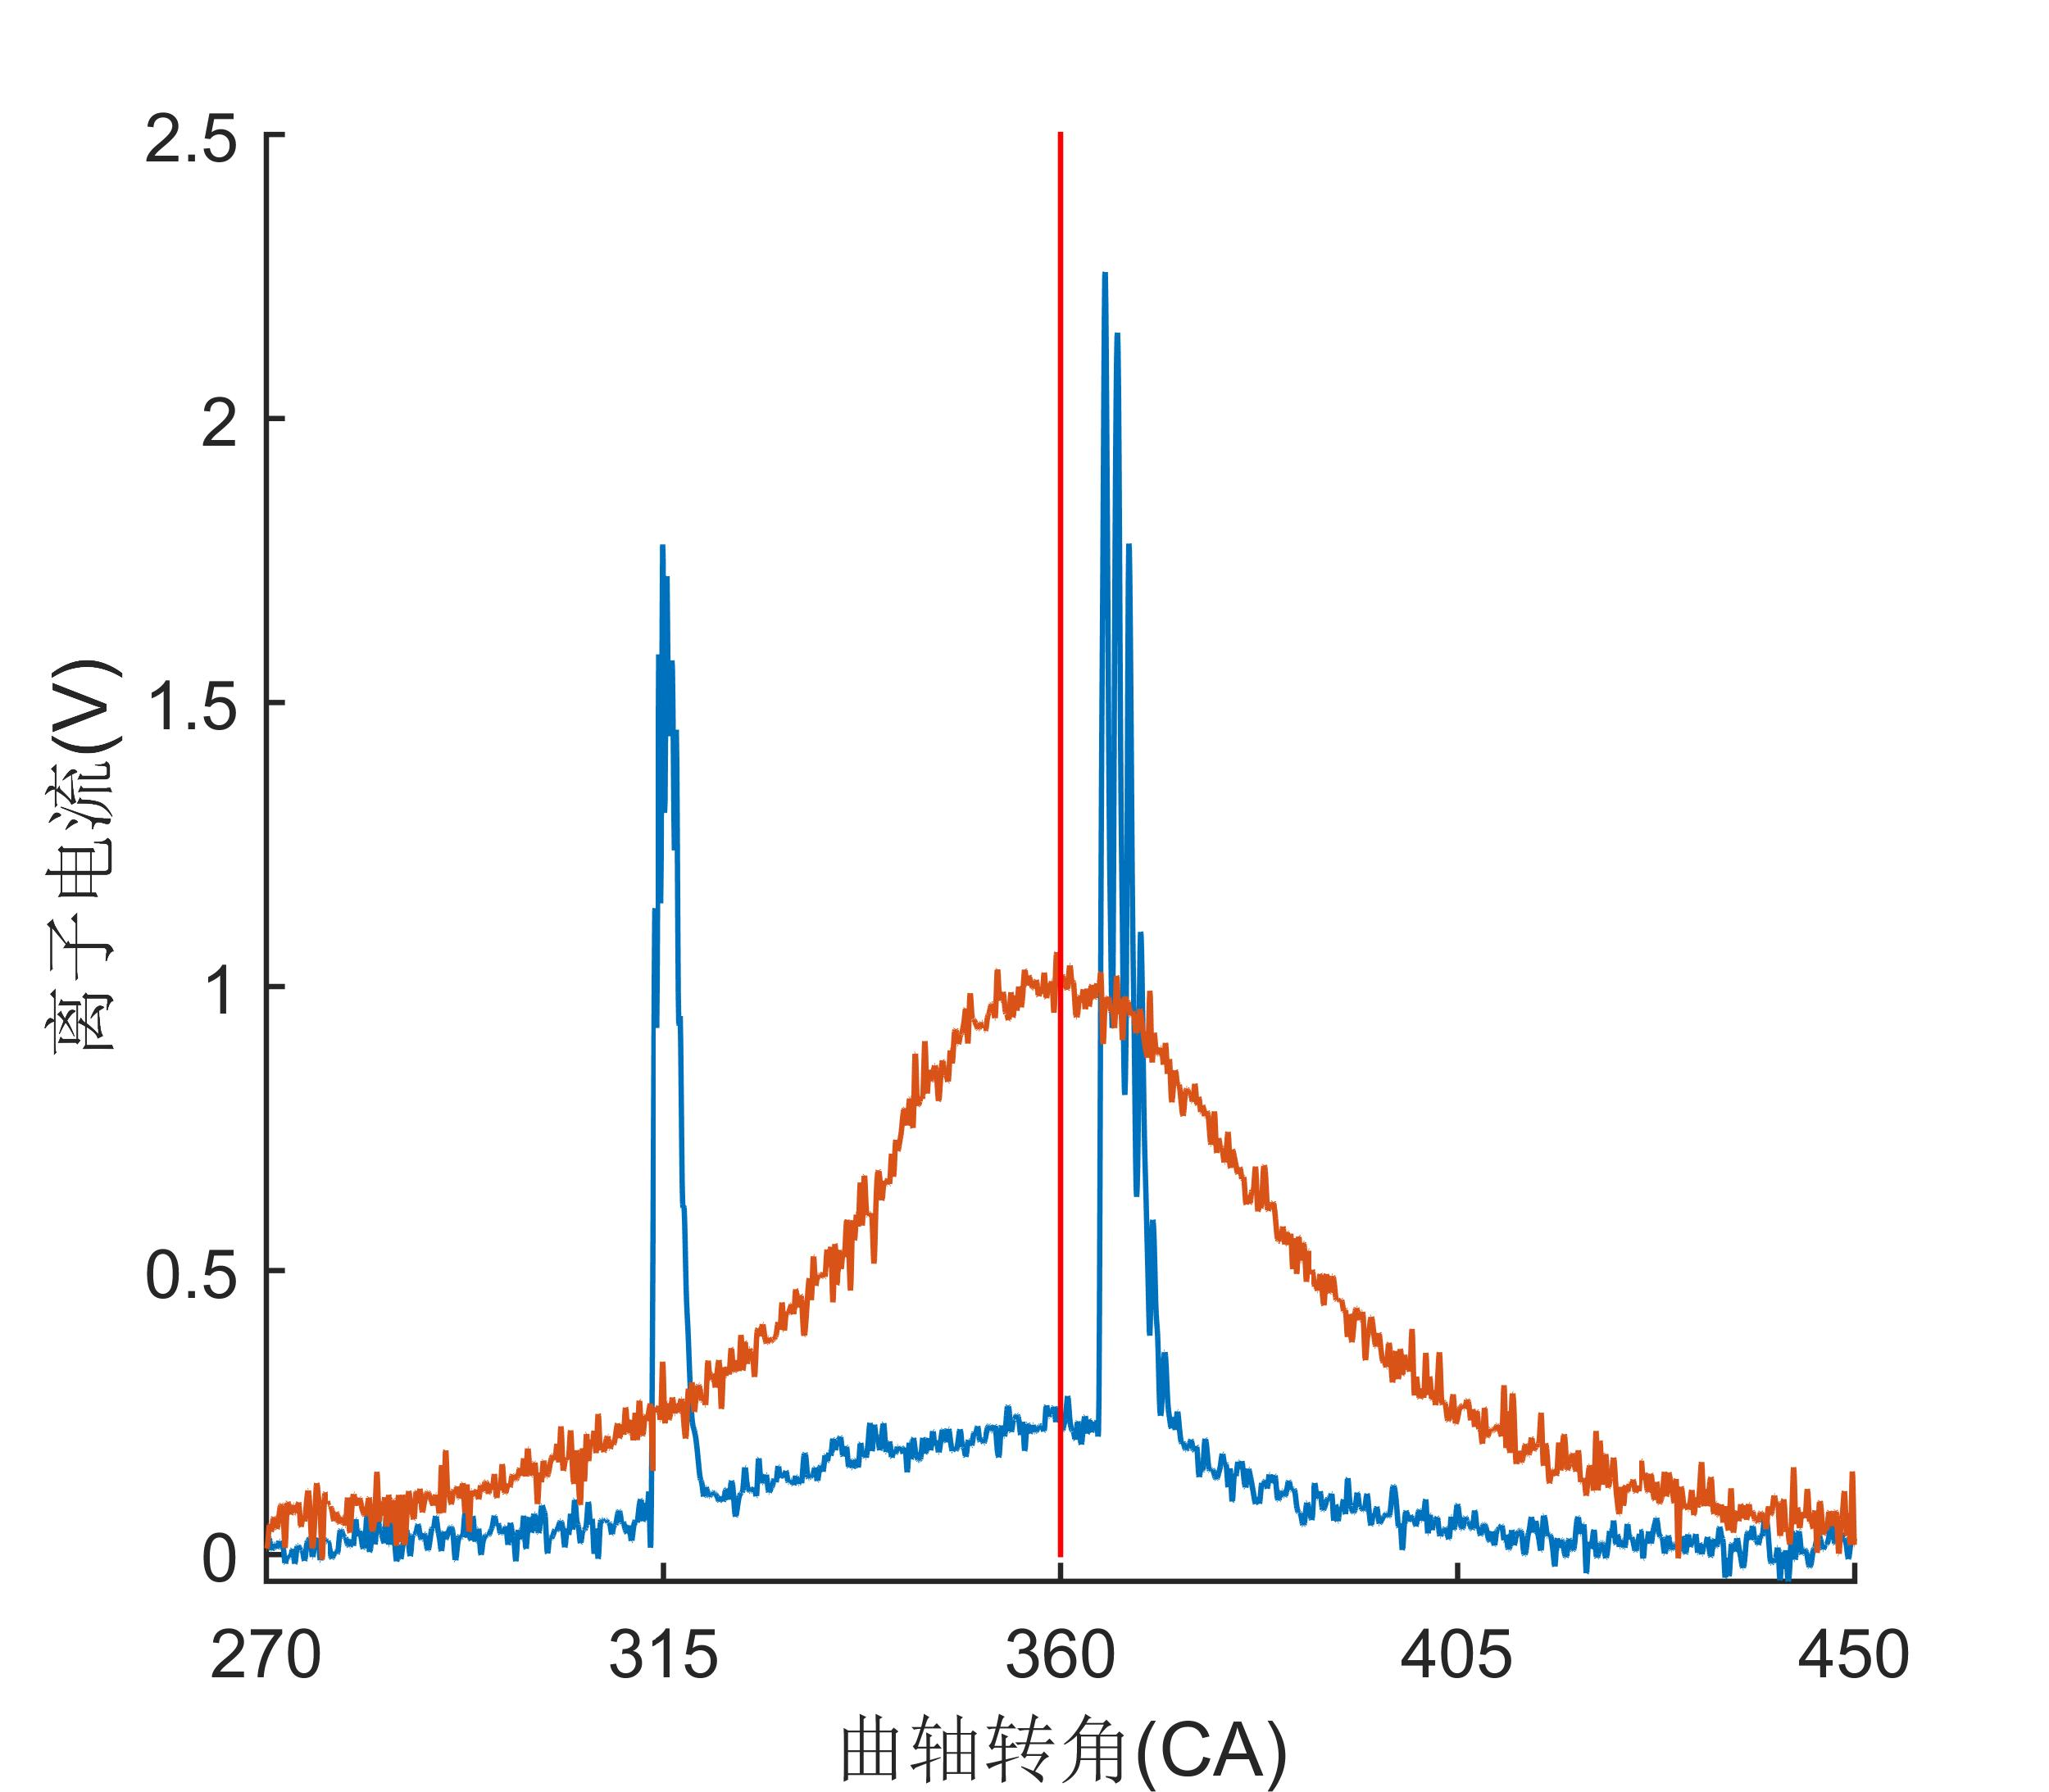
\includegraphics[width=\textwidth]{thesis_figure/ion_chapter/dy_ion}
	\caption{断油情况下的电压信号}
	\label{fig:dy_ion}
\end{minipage}
\begin{minipage}[t]{0.5\linewidth}
	\centering
	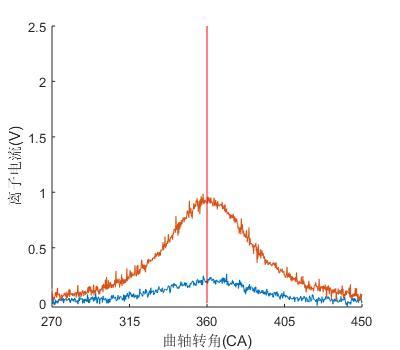
\includegraphics[width=\textwidth]{thesis_figure/ion_chapter/dh_ion}
	\caption{断火情况下的电压信号}
	\label{fig:dh_ion}
\end{minipage}
\end{figure}
\subsection{断火情况下的离子电流分析}   
当发动机断火情况下,点火线圈不进行点火过程,导致缸内混合气不能进行燃烧过程,无法形成化学电离过程的离子电流信号如图\ref{fig:dh_ion}所示是一个断火情况下的电容式检测电路检测到的电压信号。
\par 从图\ref{fig:dh_ion}中可以看到缸压曲线峰值相位在上止点360度位置,说明该循环处于纯压缩循环。可以看到此时的离子电流信号的峰值相位也是上止点位置,此时的离子电流信号是热电离导致的,没有化学电离产生的离子电流信号。
\subsection{纯点火干扰的分析方法}
对比图\ref{fig:dy_ion}和图\ref{fig:dh_ion},可以看到无论断油还是断火,都会导致缸内的混合气体无法燃烧,不能够产生化学电离,两者的循环都是纯压缩循环。
同时热电离曲线的形状和峰值大小都类似。所以可以将同一转速和负荷下的离子电流信号相减,即可得到近似的纯点火干扰信号。
\begin{figure}[ht]
\begin{minipage}[t]{0.5\linewidth}
	\centering
	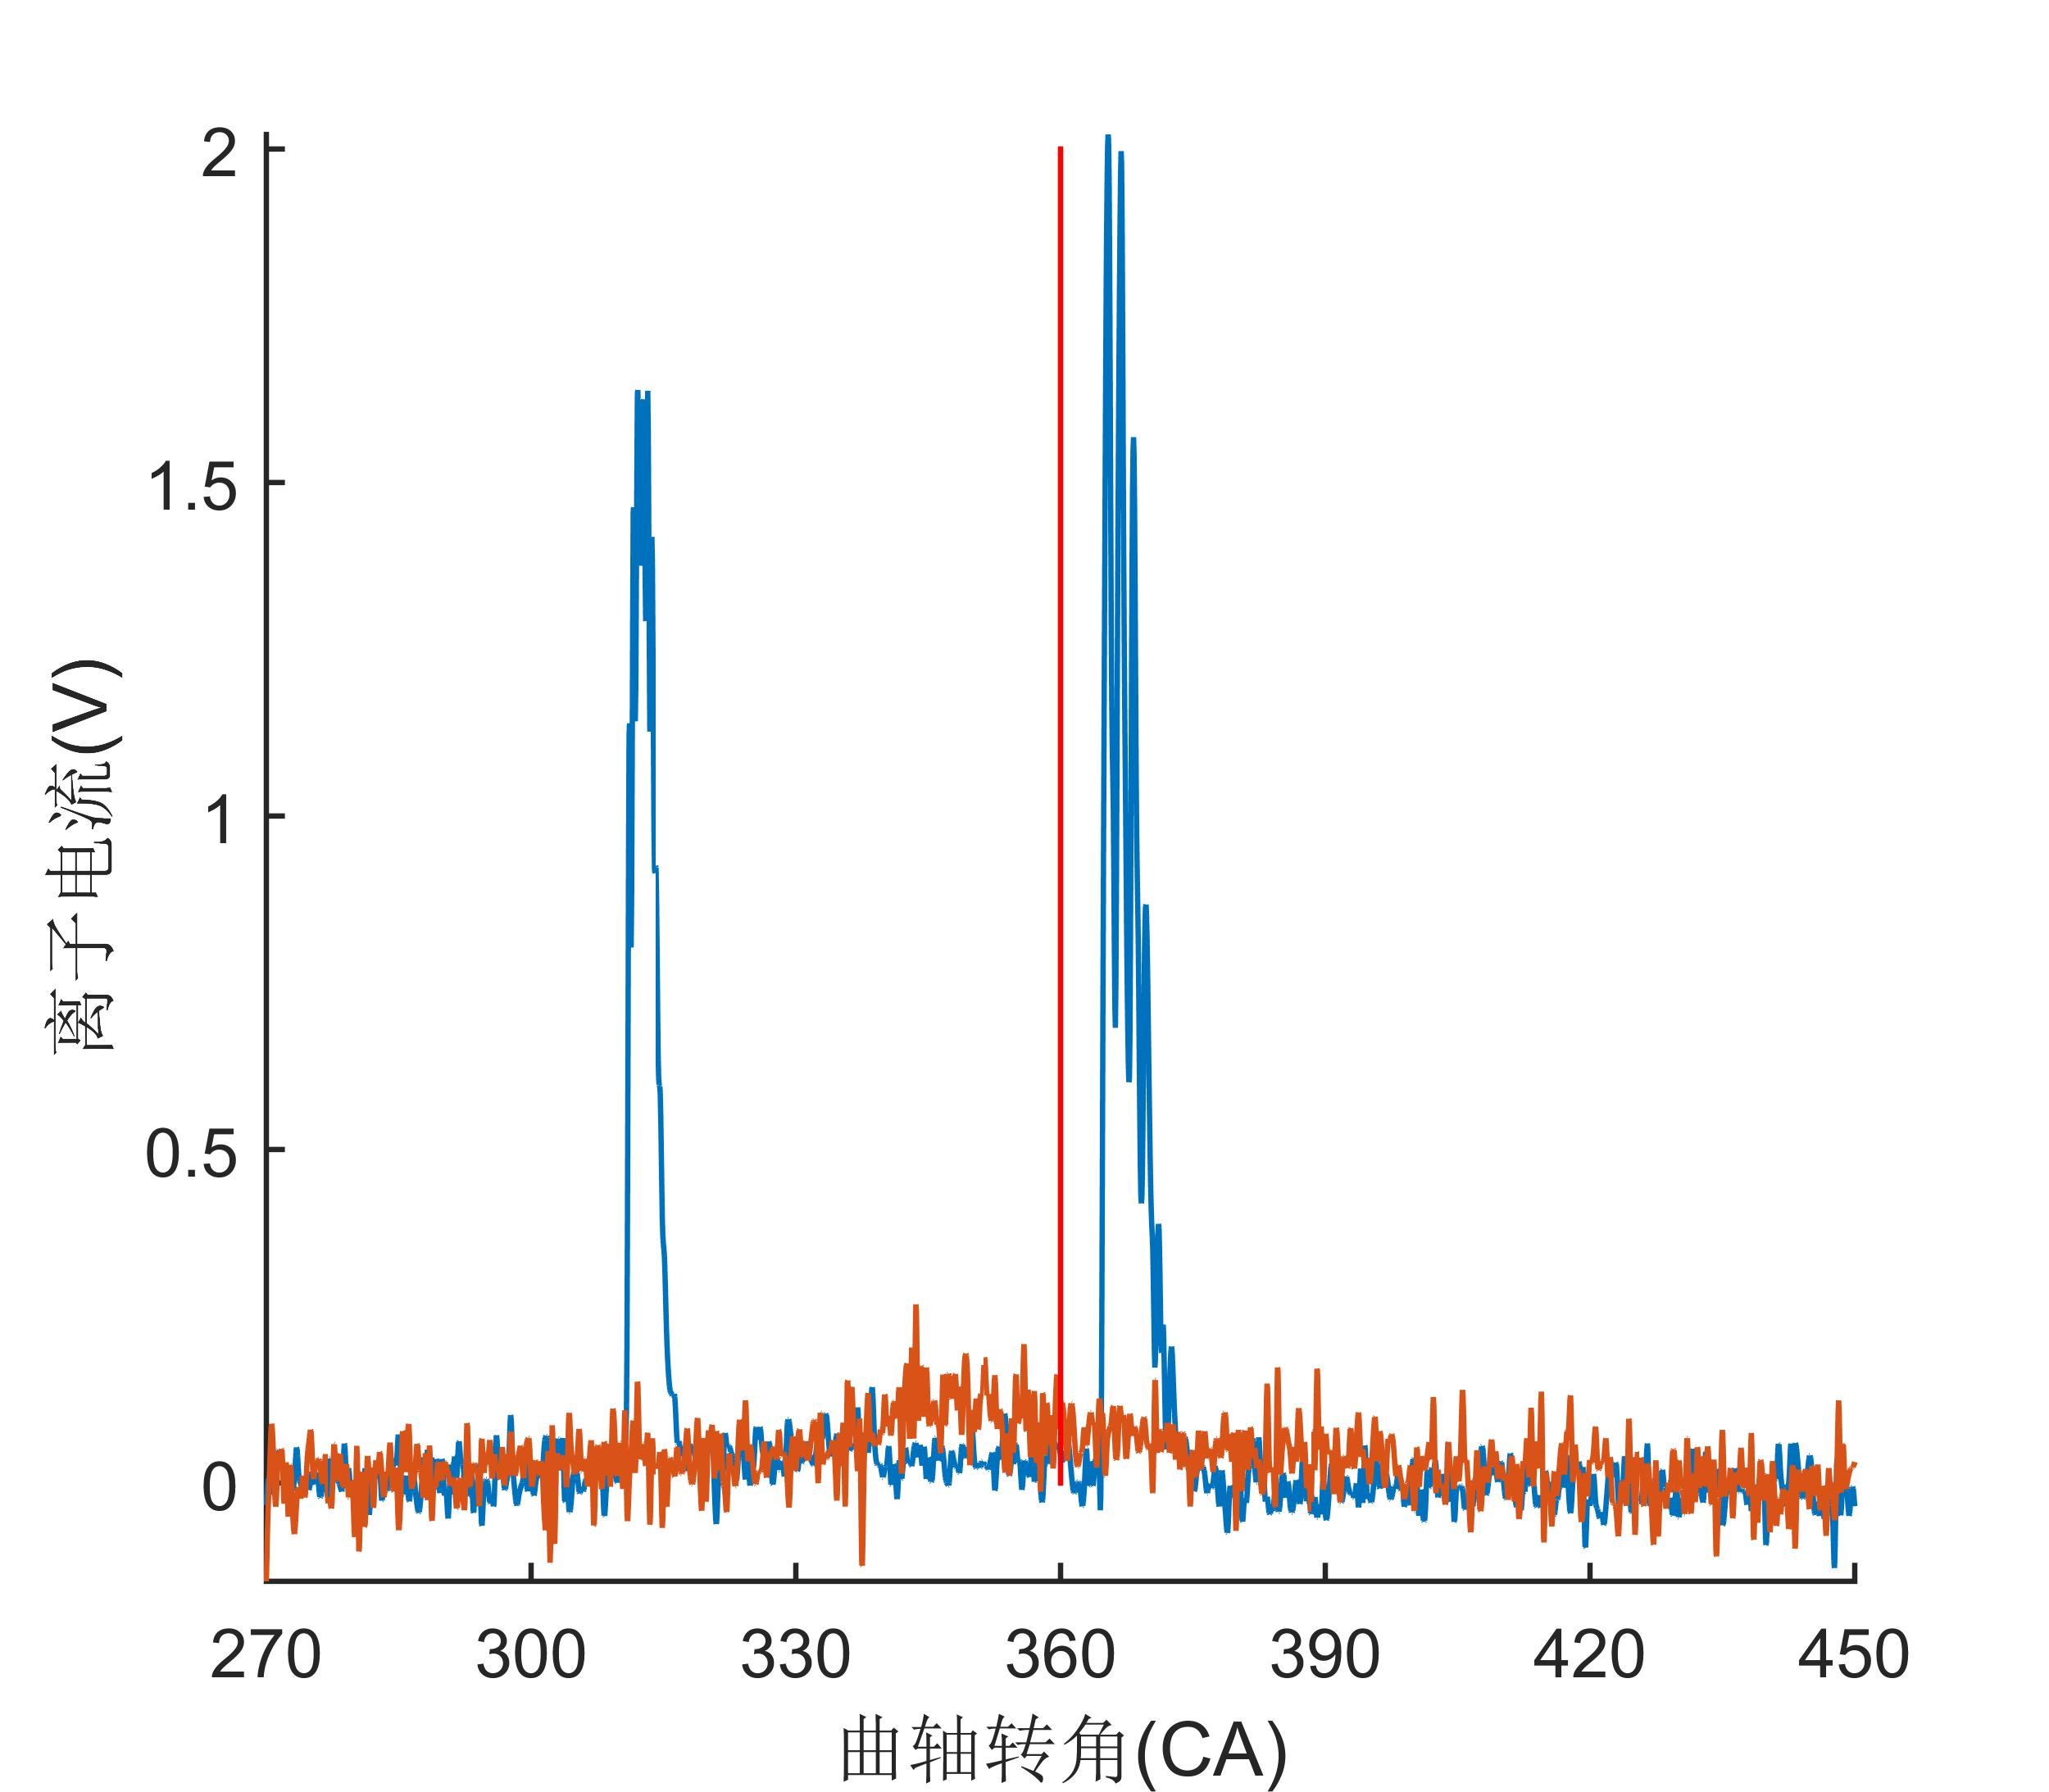
\includegraphics[width=\textwidth]{thesis_figure/ion_chapter/diff_dy_dh}
\end{minipage}
\begin{minipage}[t]{0.5\linewidth}
	\centering
	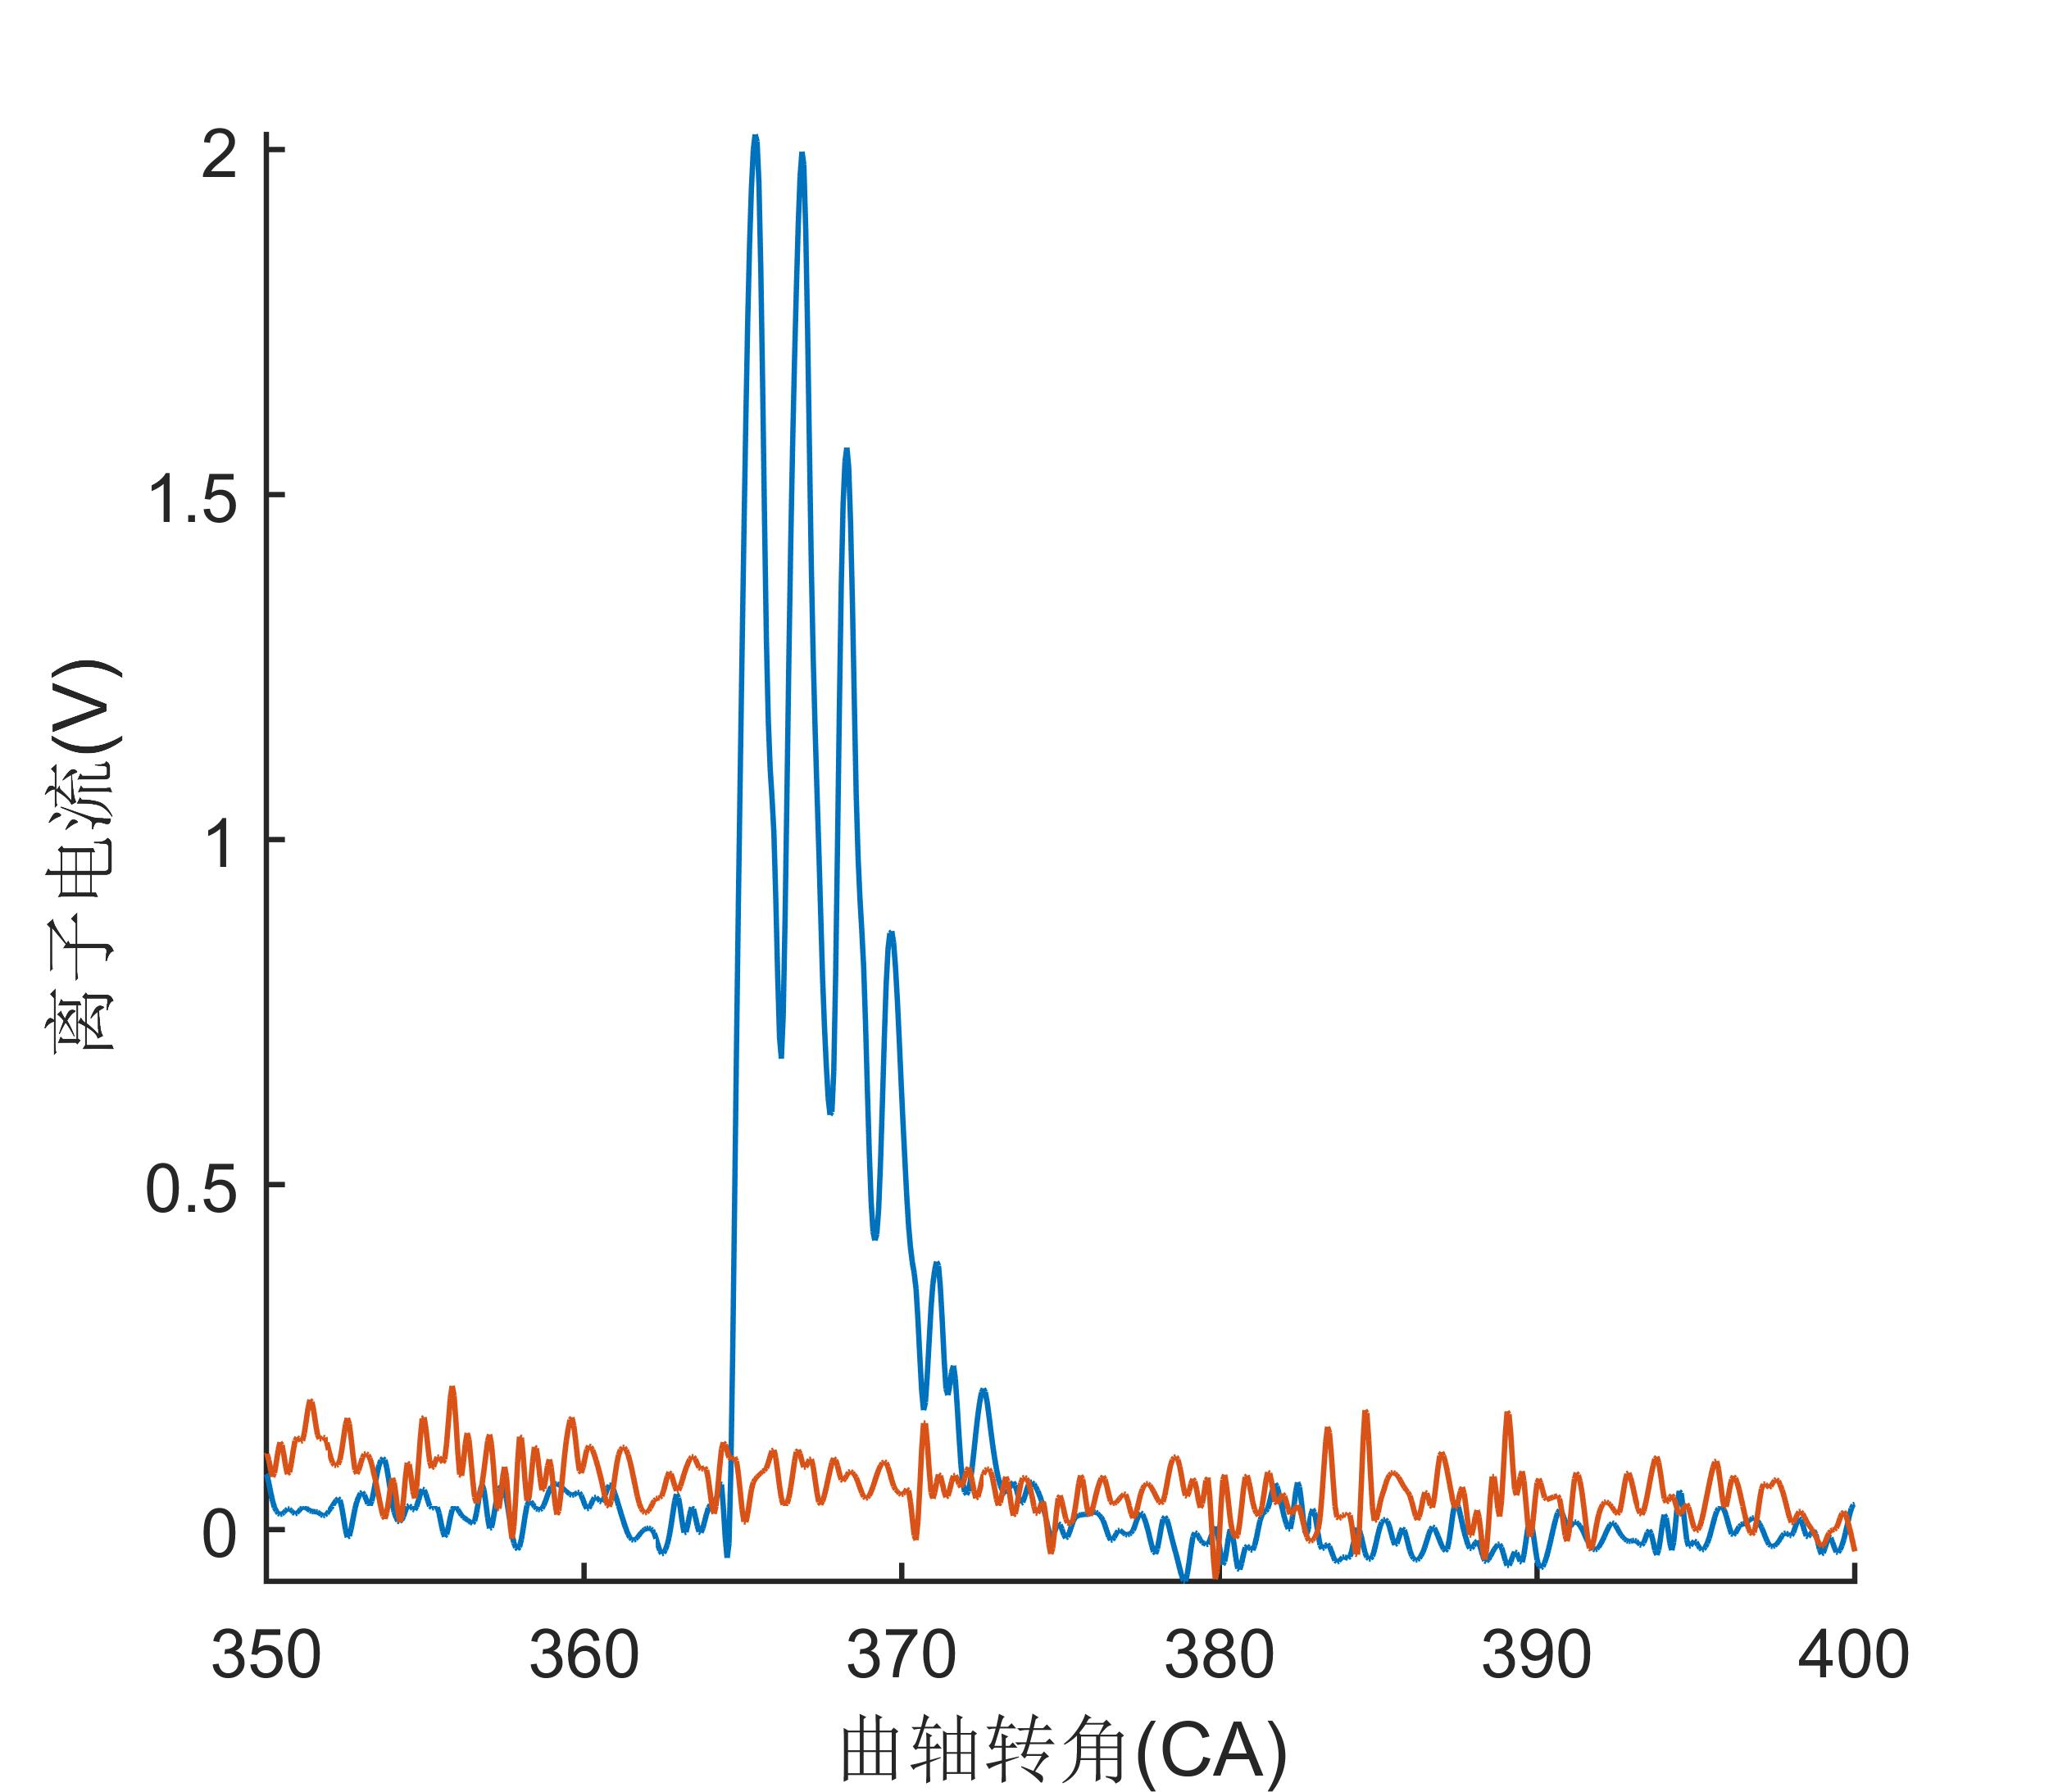
\includegraphics[width=\textwidth]{thesis_figure/ion_chapter/diff_dy_dh_detail}
\end{minipage}
	\caption{断油离子电流信号与断火离子电流信号差值}
	\label{fig:diff_dy_dh}
\end{figure}
如图\ref{fig:diff_dy_dh}所示可以得到近似的纯点火干扰信号。可以看到两者的缸压曲线也是近似的,说明在同一个工况下的断油和断火循环,造成的缸内情况是类似的,因此两者相减得到的离子电流信号在一定
程度上是可以表征纯电火干扰信号的。
\begin{figure}[H]
	\centering
	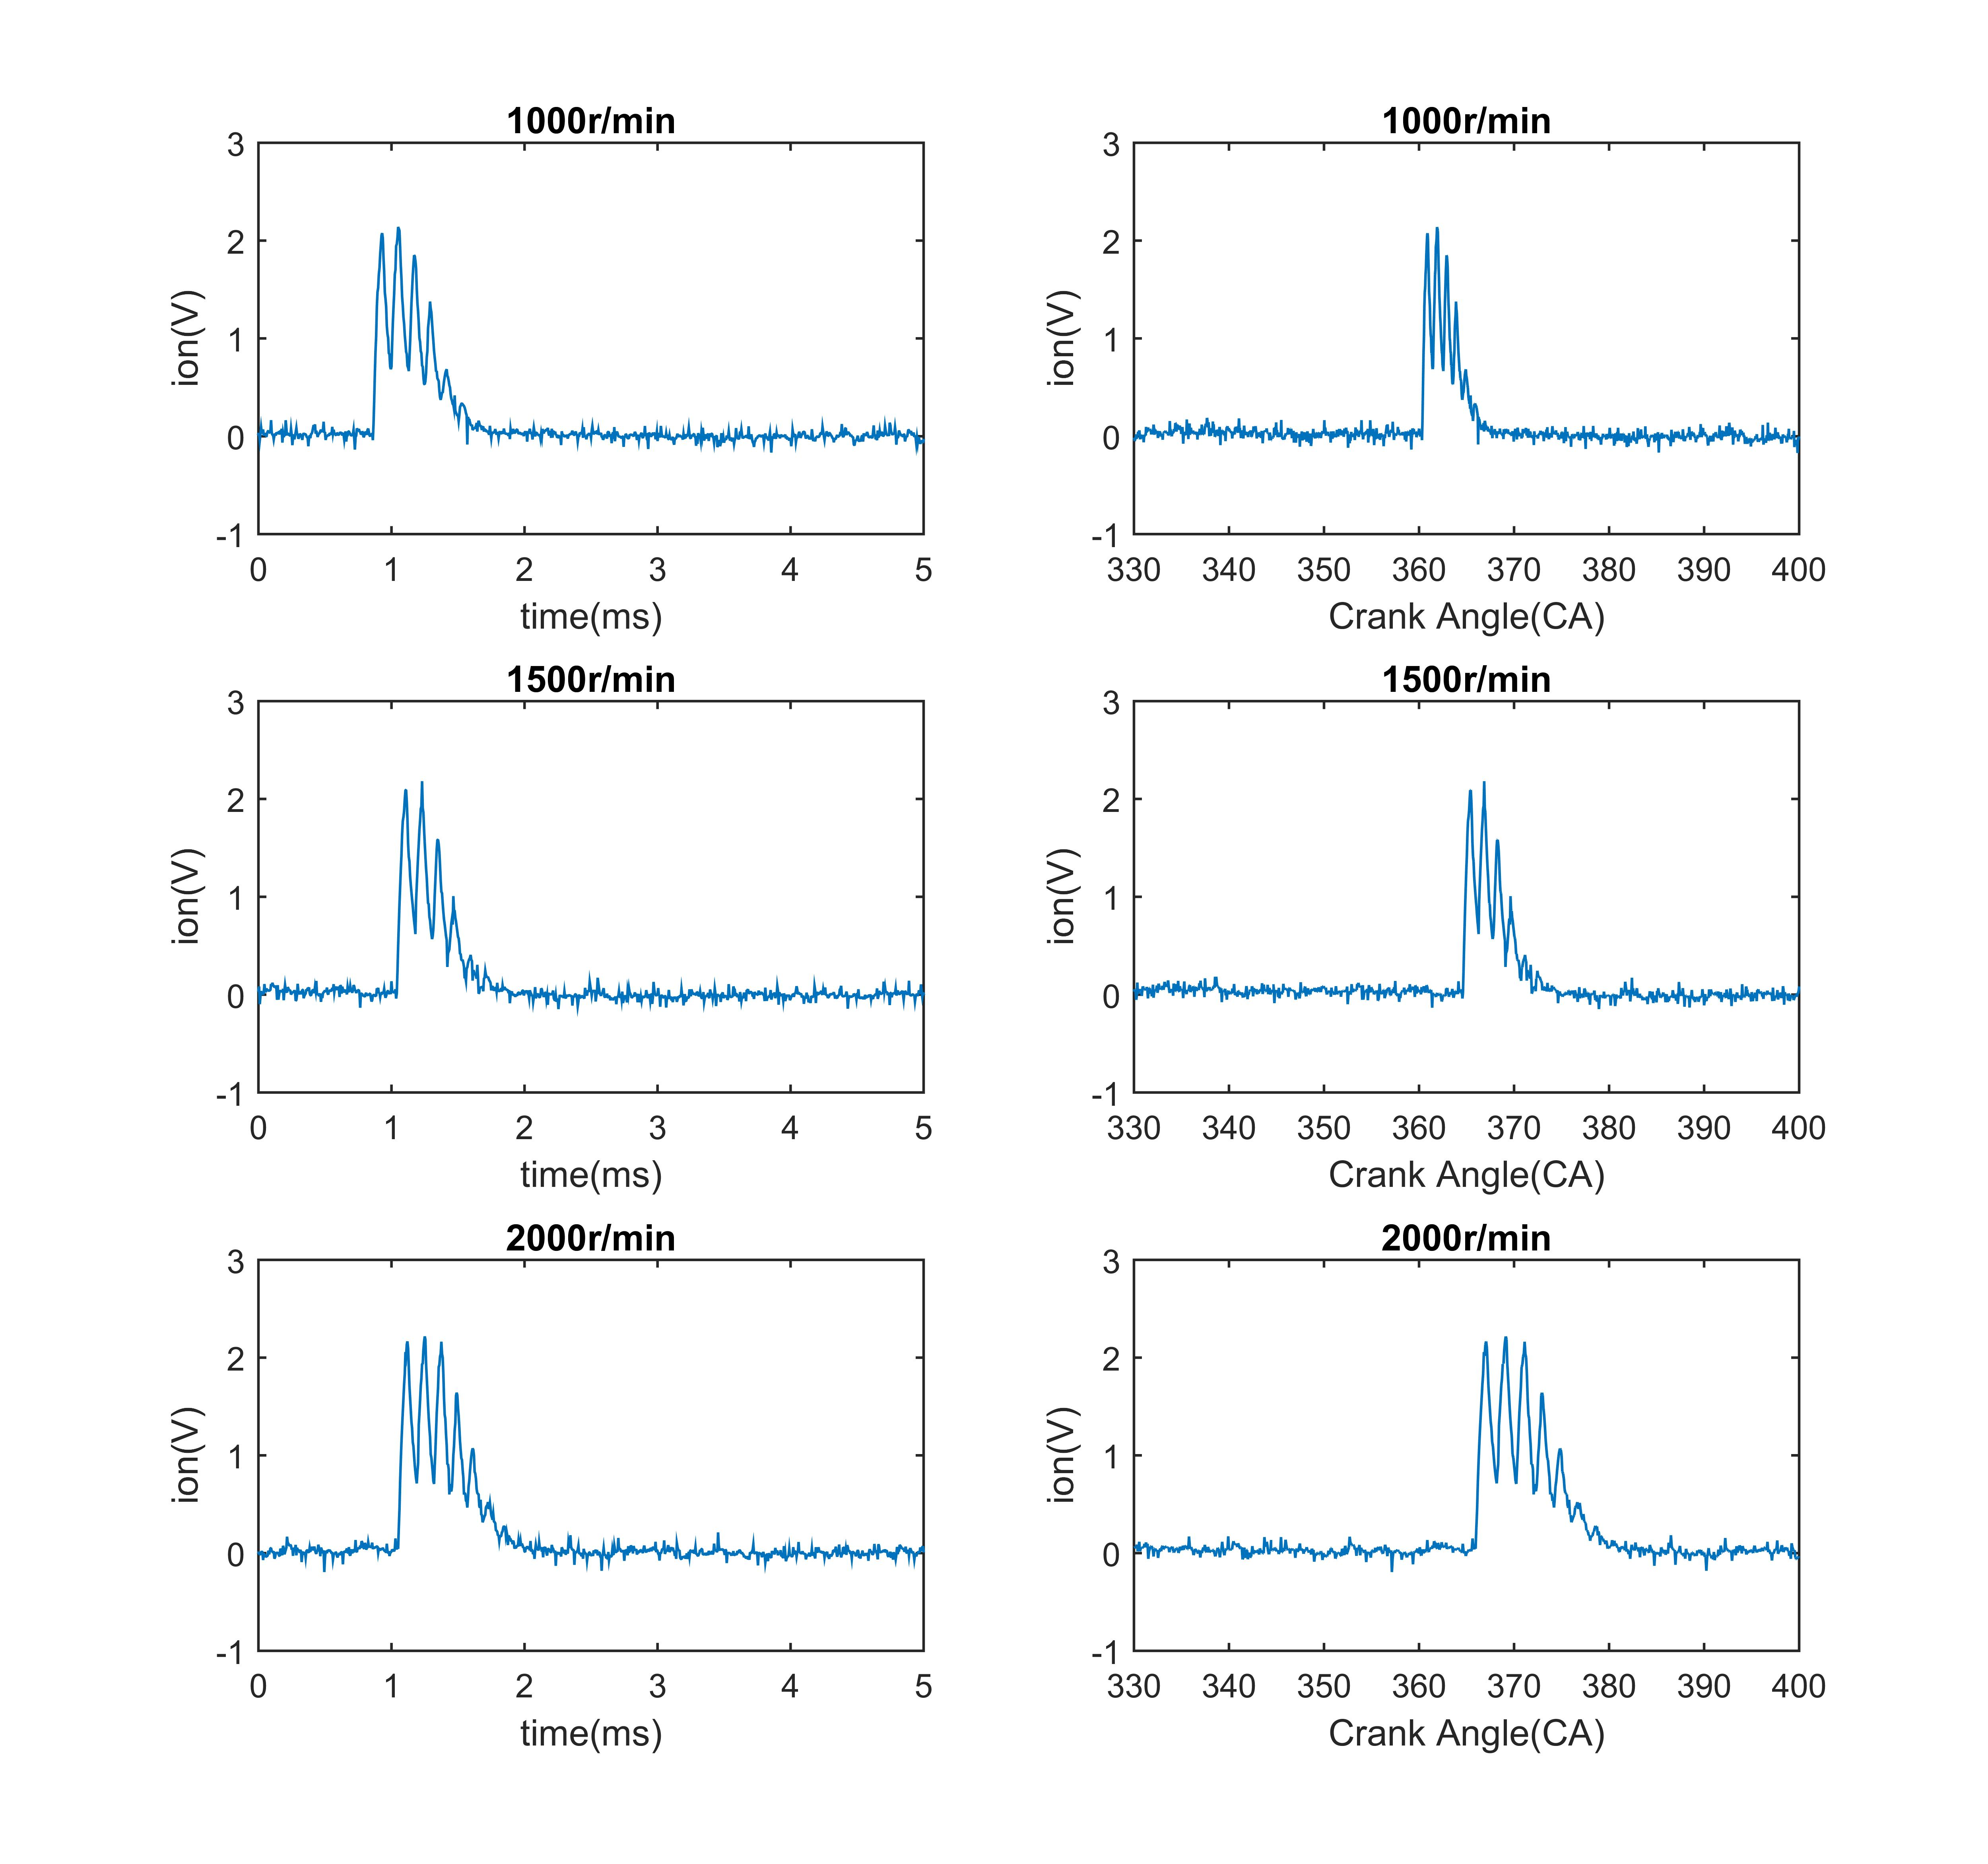
\includegraphics[width=0.9\textwidth]{thesis_figure/ion_chapter/pure_ign_comparison}
	\caption{三种转速下的纯点火干扰的时间窗口对比和曲轴转角窗口对比}
	\label{fig:pure_ign_comparison}
\end{figure}
\par 为了验证该信号的偶然性,我们选取了$1250r/min,1500r/min,2000r/min$三种转速下50\%负荷情况下的同一次实验中同时进行断油和断火操作,得到三个纯点火干扰信号。
从图\ref{fig:pure_ign_comparison}中可以看到纯点火干扰在时间窗口上具有很相近的形状,但是仍然有细节上的差异,如果用正常信号直接减去该纯点火干扰信号并不能非常完美的呈现出离子电流信号。有必要通过
其他的信号分析手段来将该点火干扰信号剔除。
\section{四种小波基函数对点火干扰进行小波分析}
小波分析的方法可以很好的将高频信号和低频信号进行分离,我们采用db,sym,coif,dmey四种离散小波基函数对纯电火干扰信号进行分析,将纯点火干扰信号中的震荡信号去除。
\begin{figure}[!htb]
	\begin{tabular}{lll}
		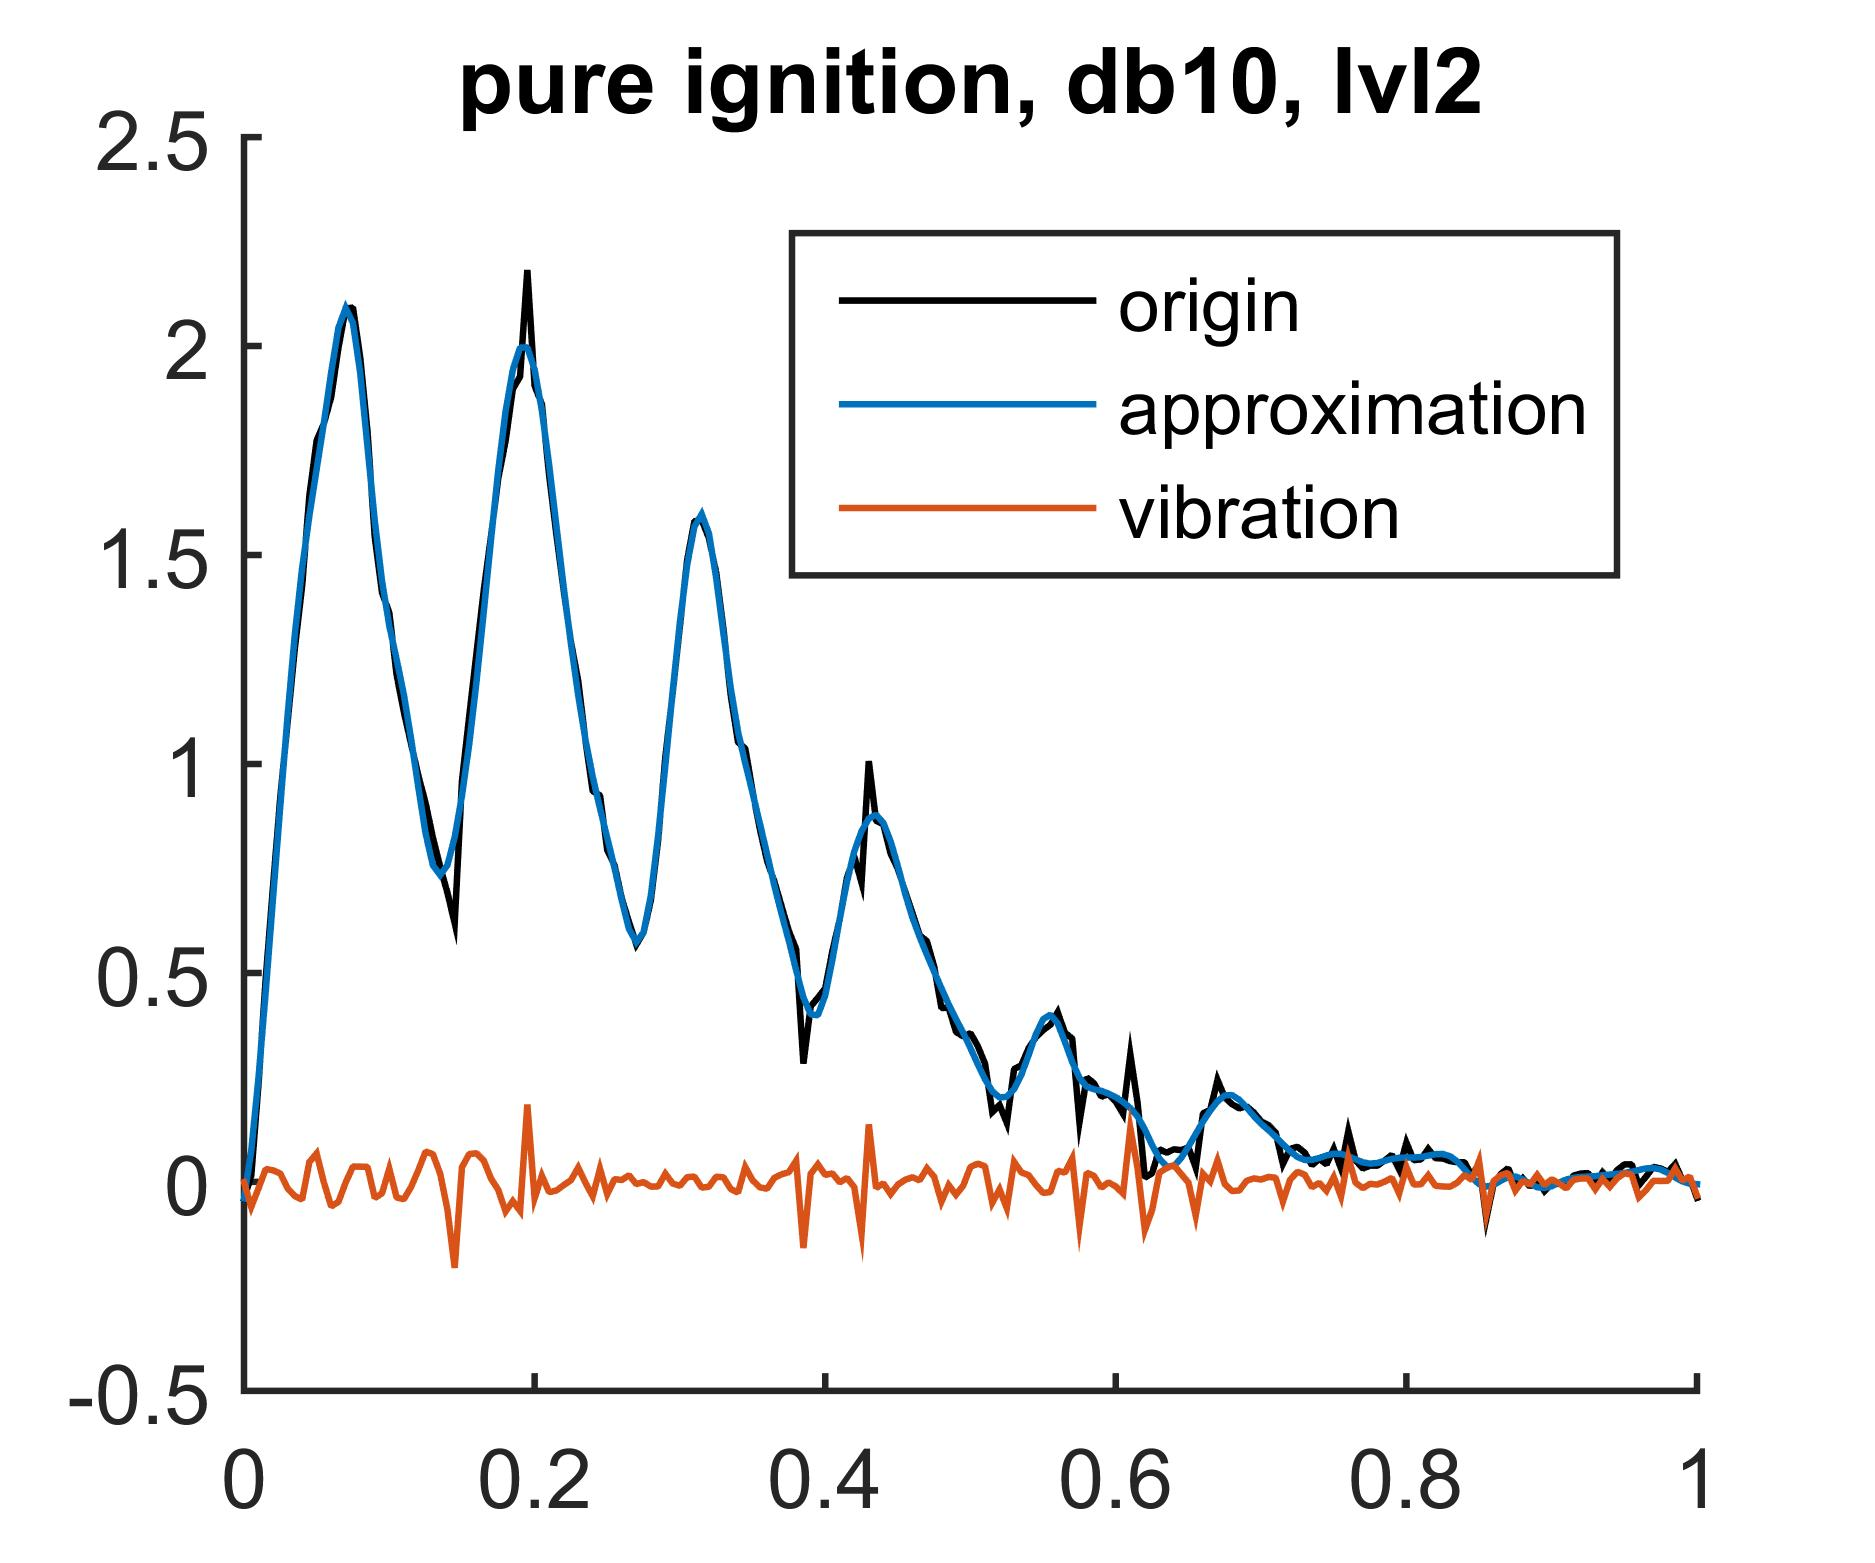
\includegraphics[width=0.3\textwidth]{thesis_figure/ion_chapter/db10_lvl2}&
		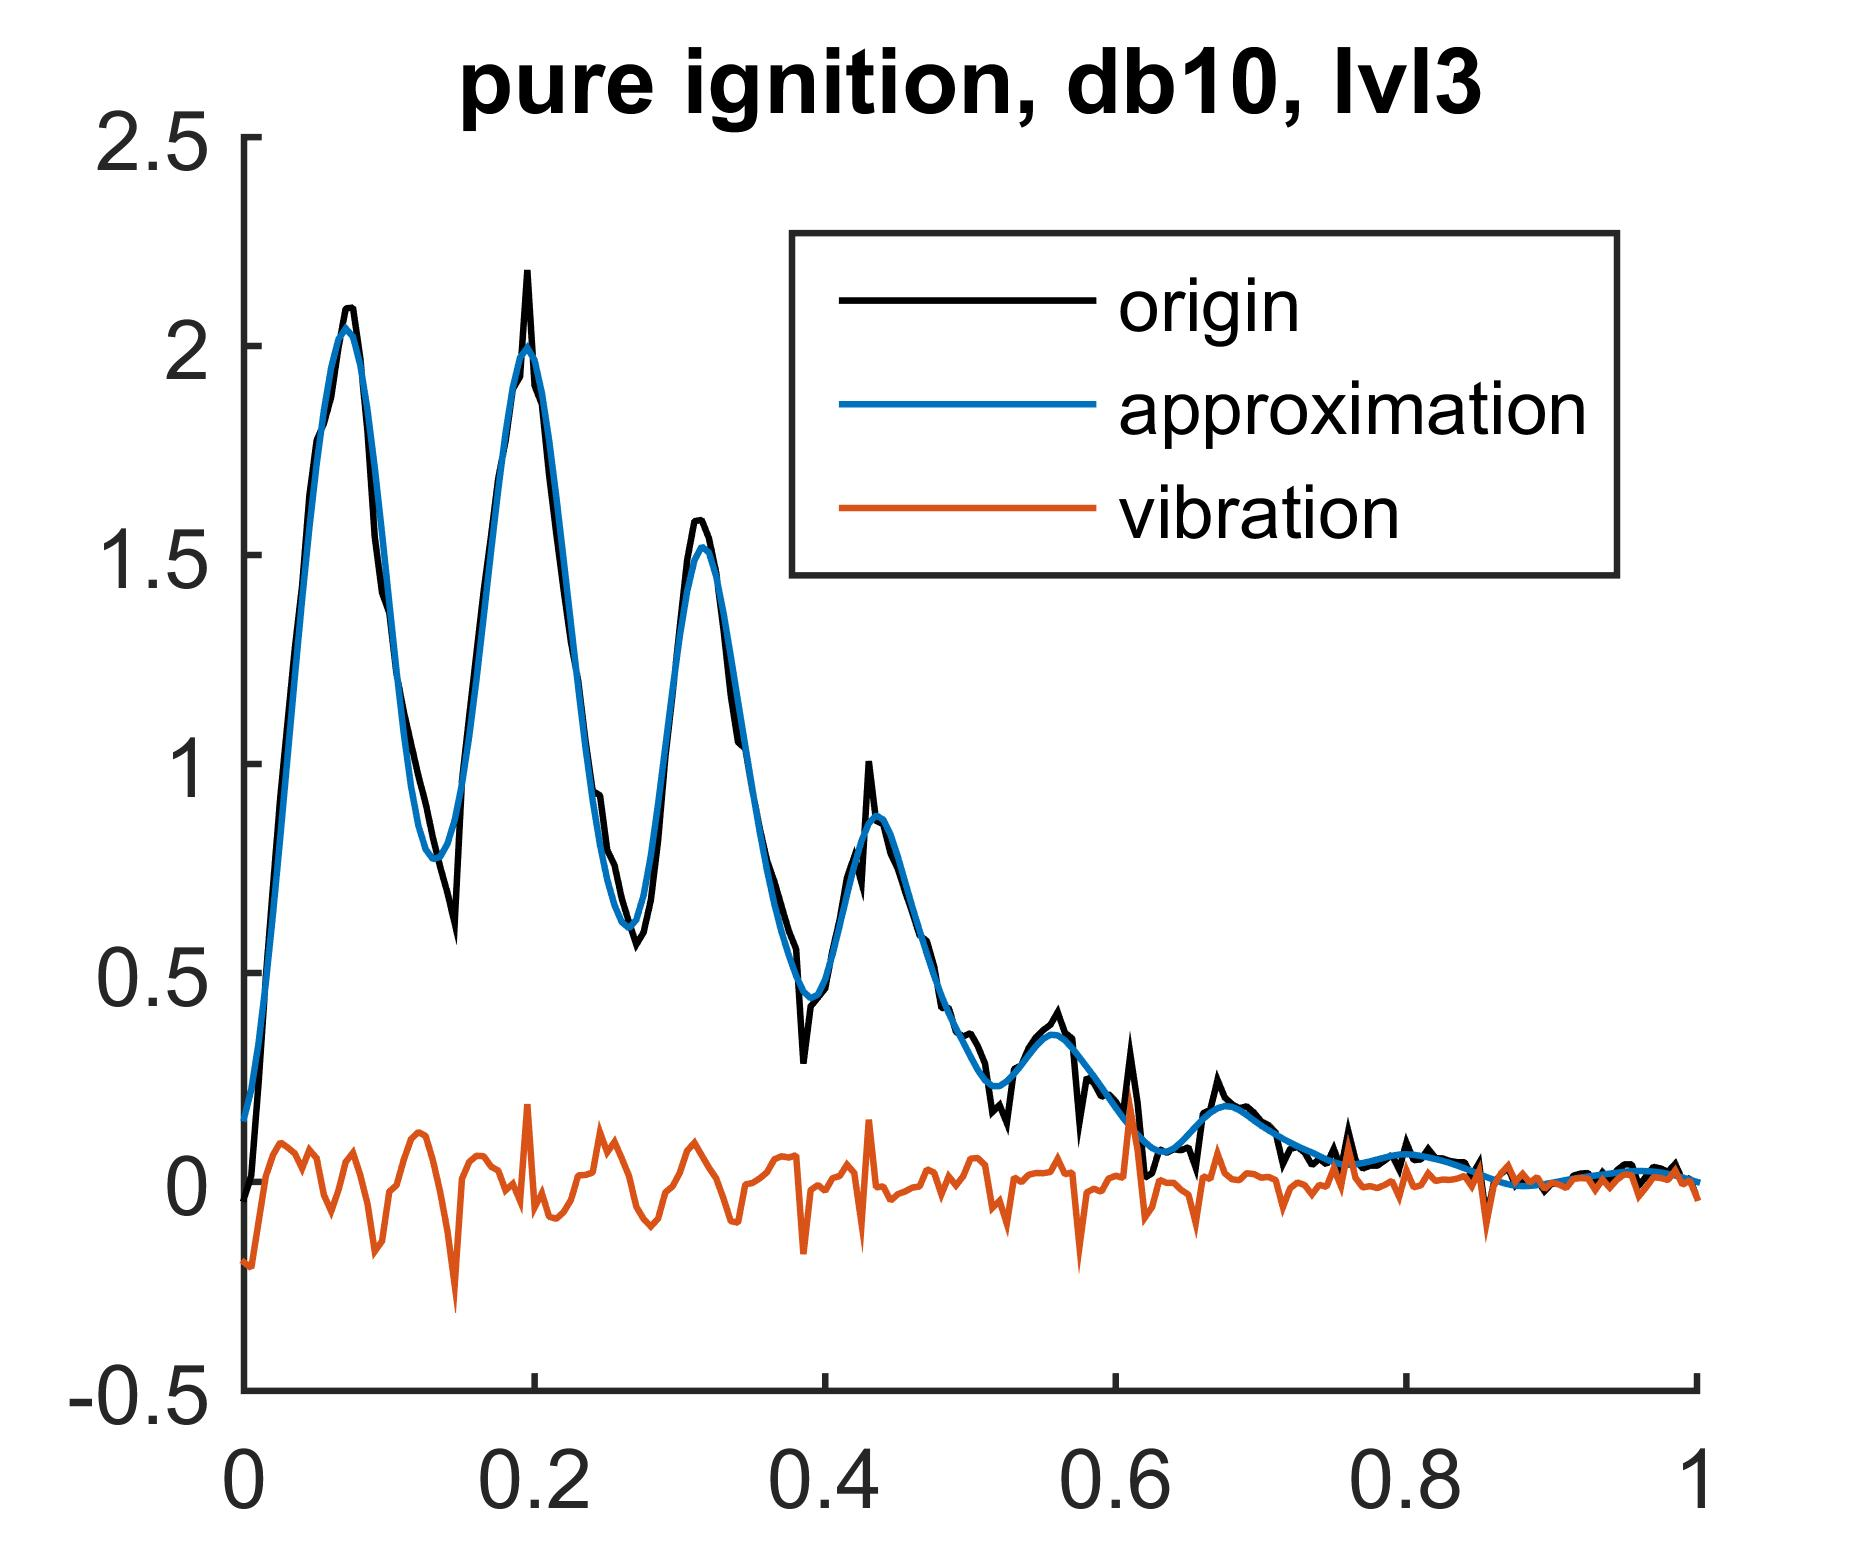
\includegraphics[width=0.3\textwidth]{thesis_figure/ion_chapter/db10_lvl3}&
		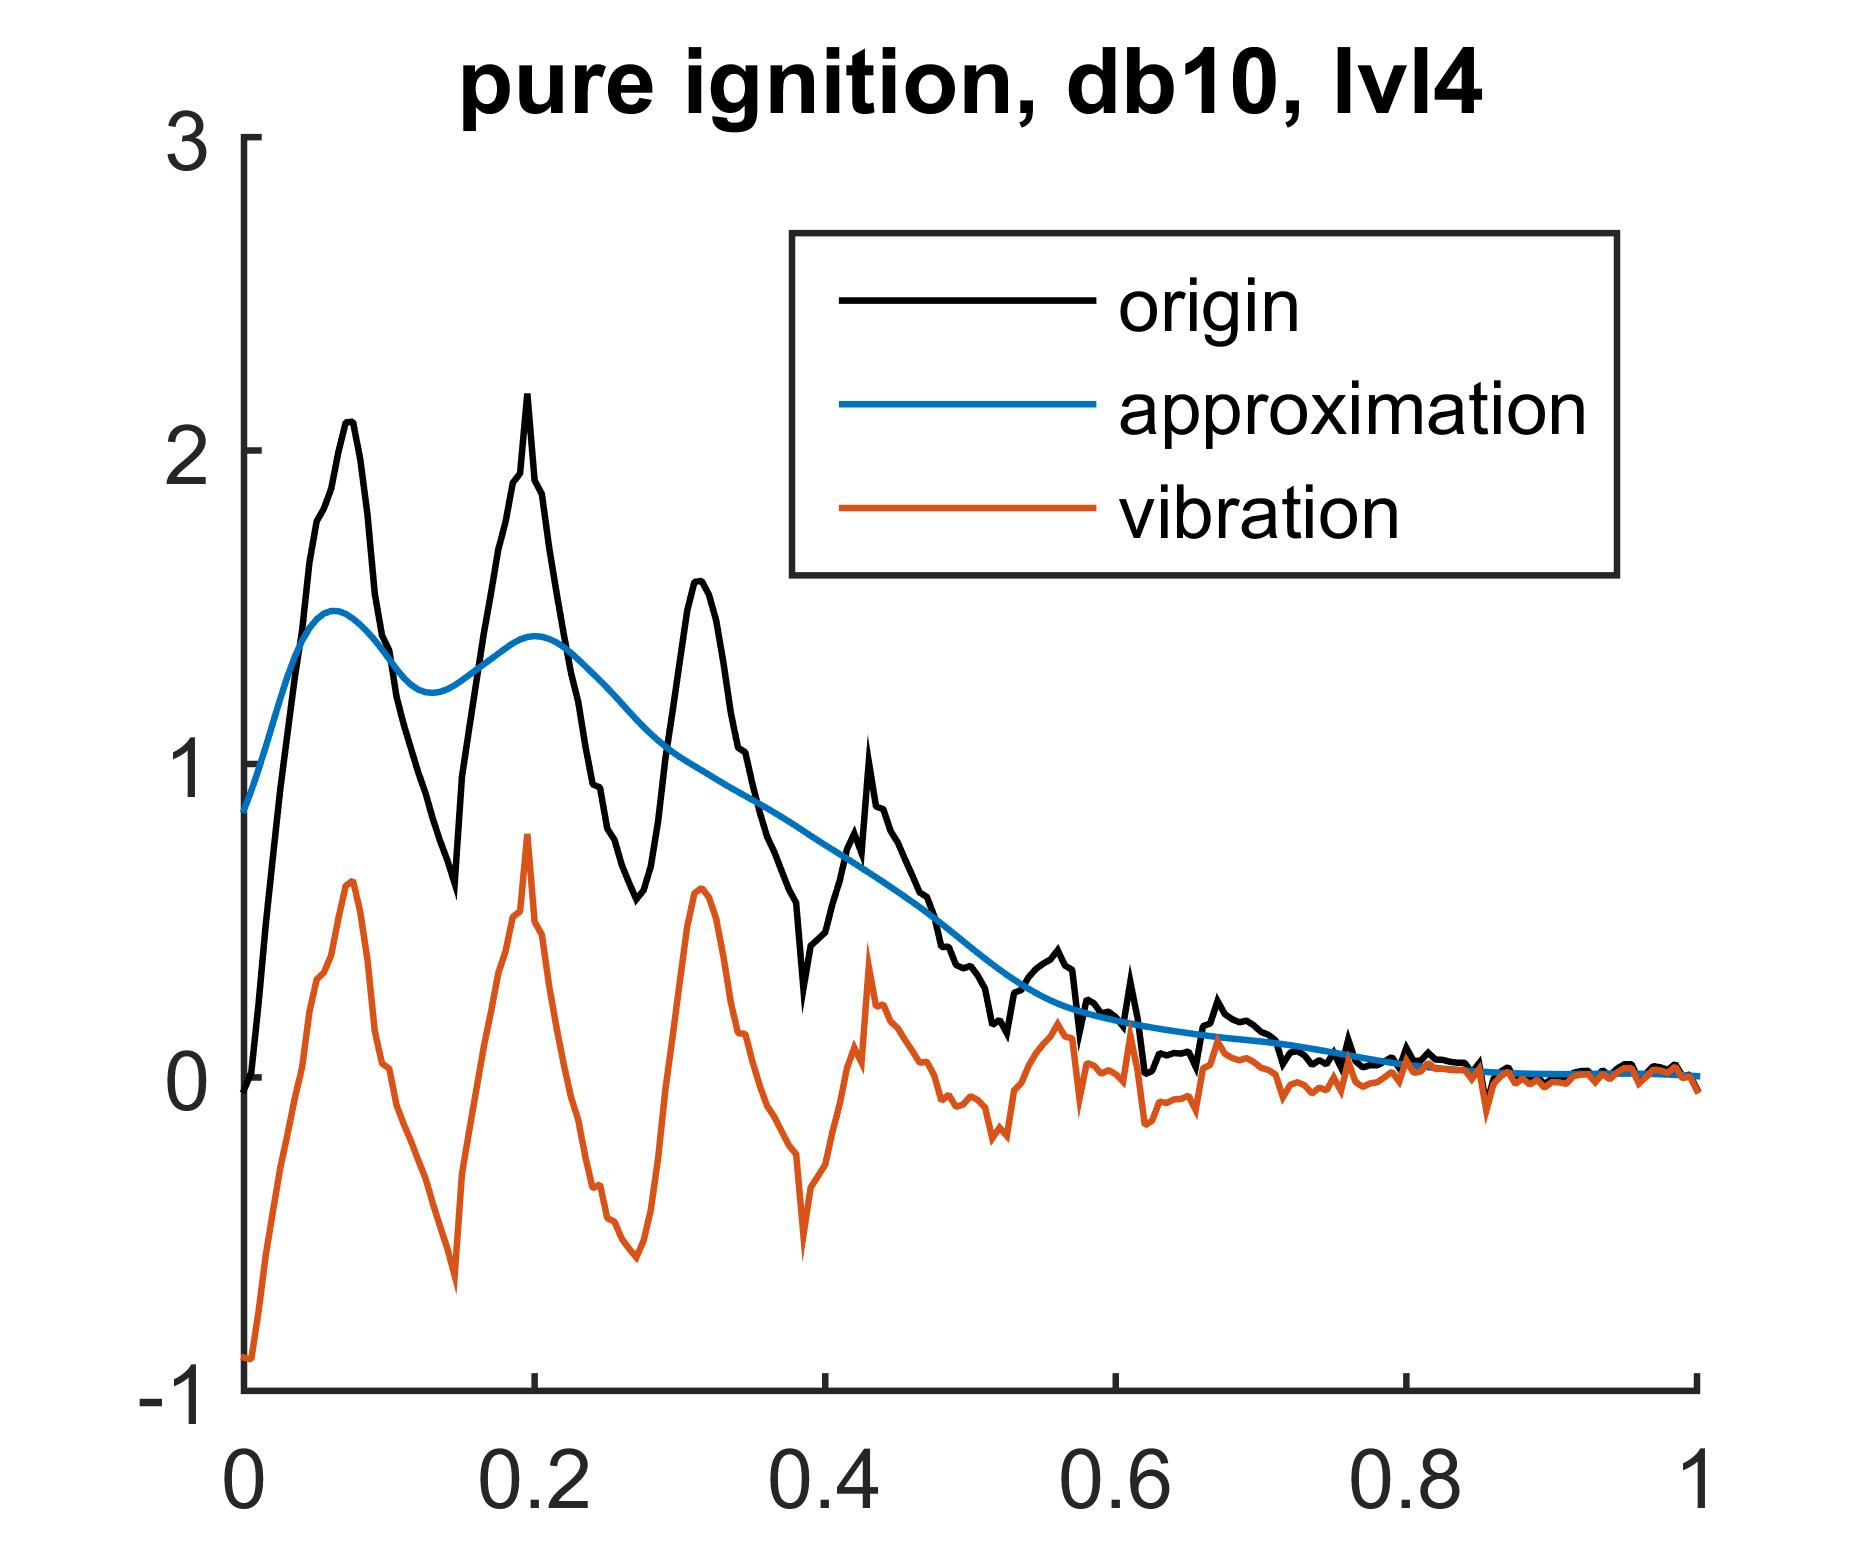
\includegraphics[width=0.3\textwidth]{thesis_figure/ion_chapter/db10_lvl4}\\
		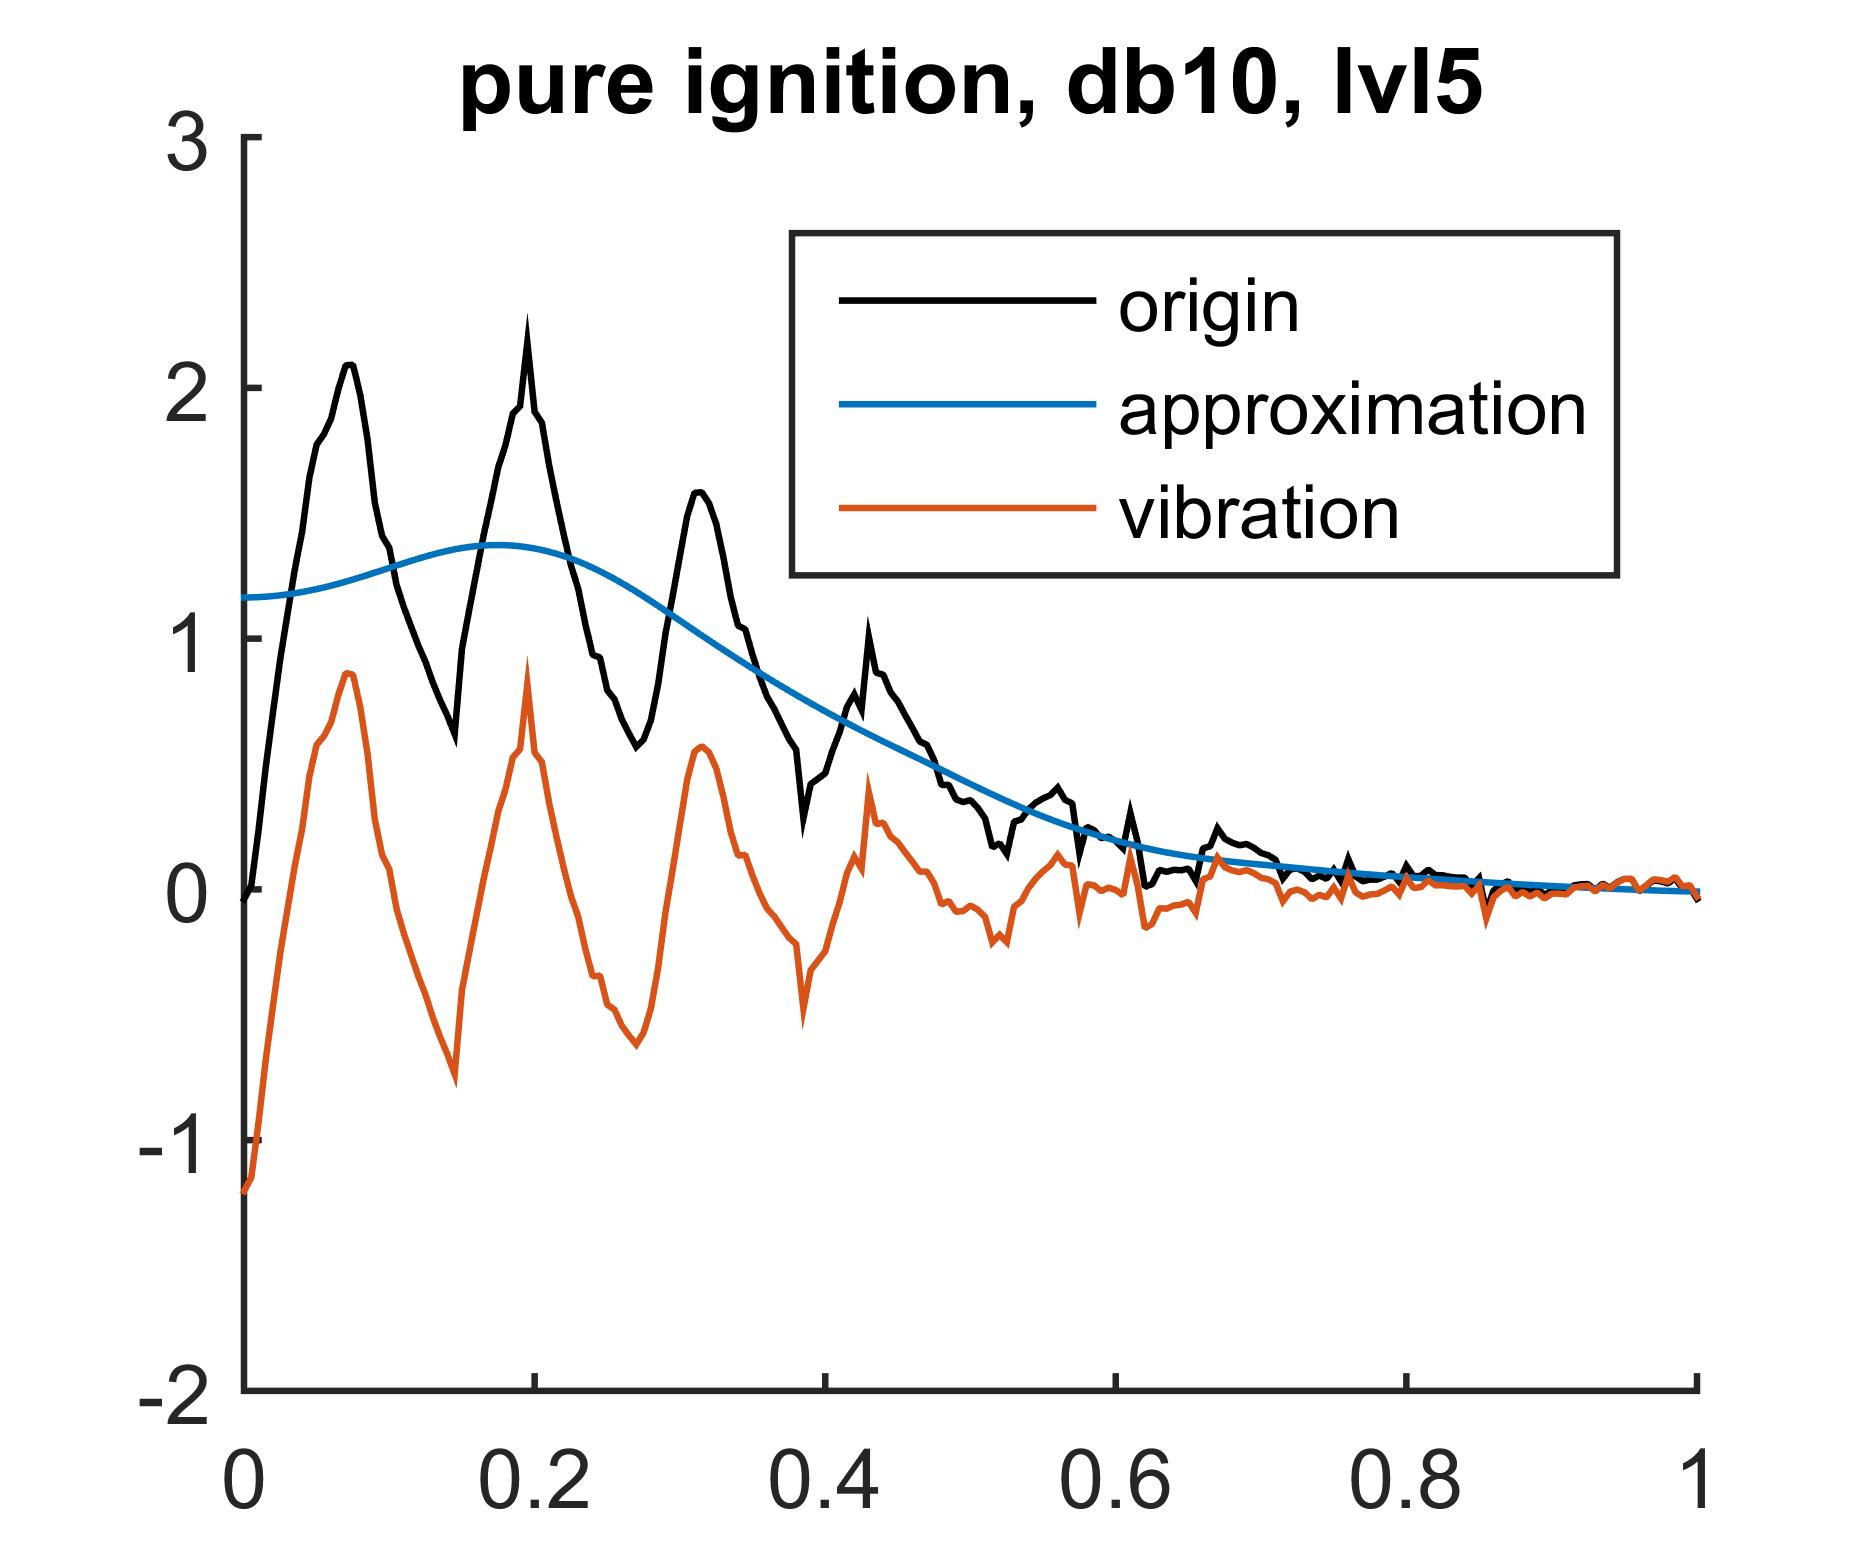
\includegraphics[width=0.3\textwidth]{thesis_figure/ion_chapter/db10_lvl5}&
		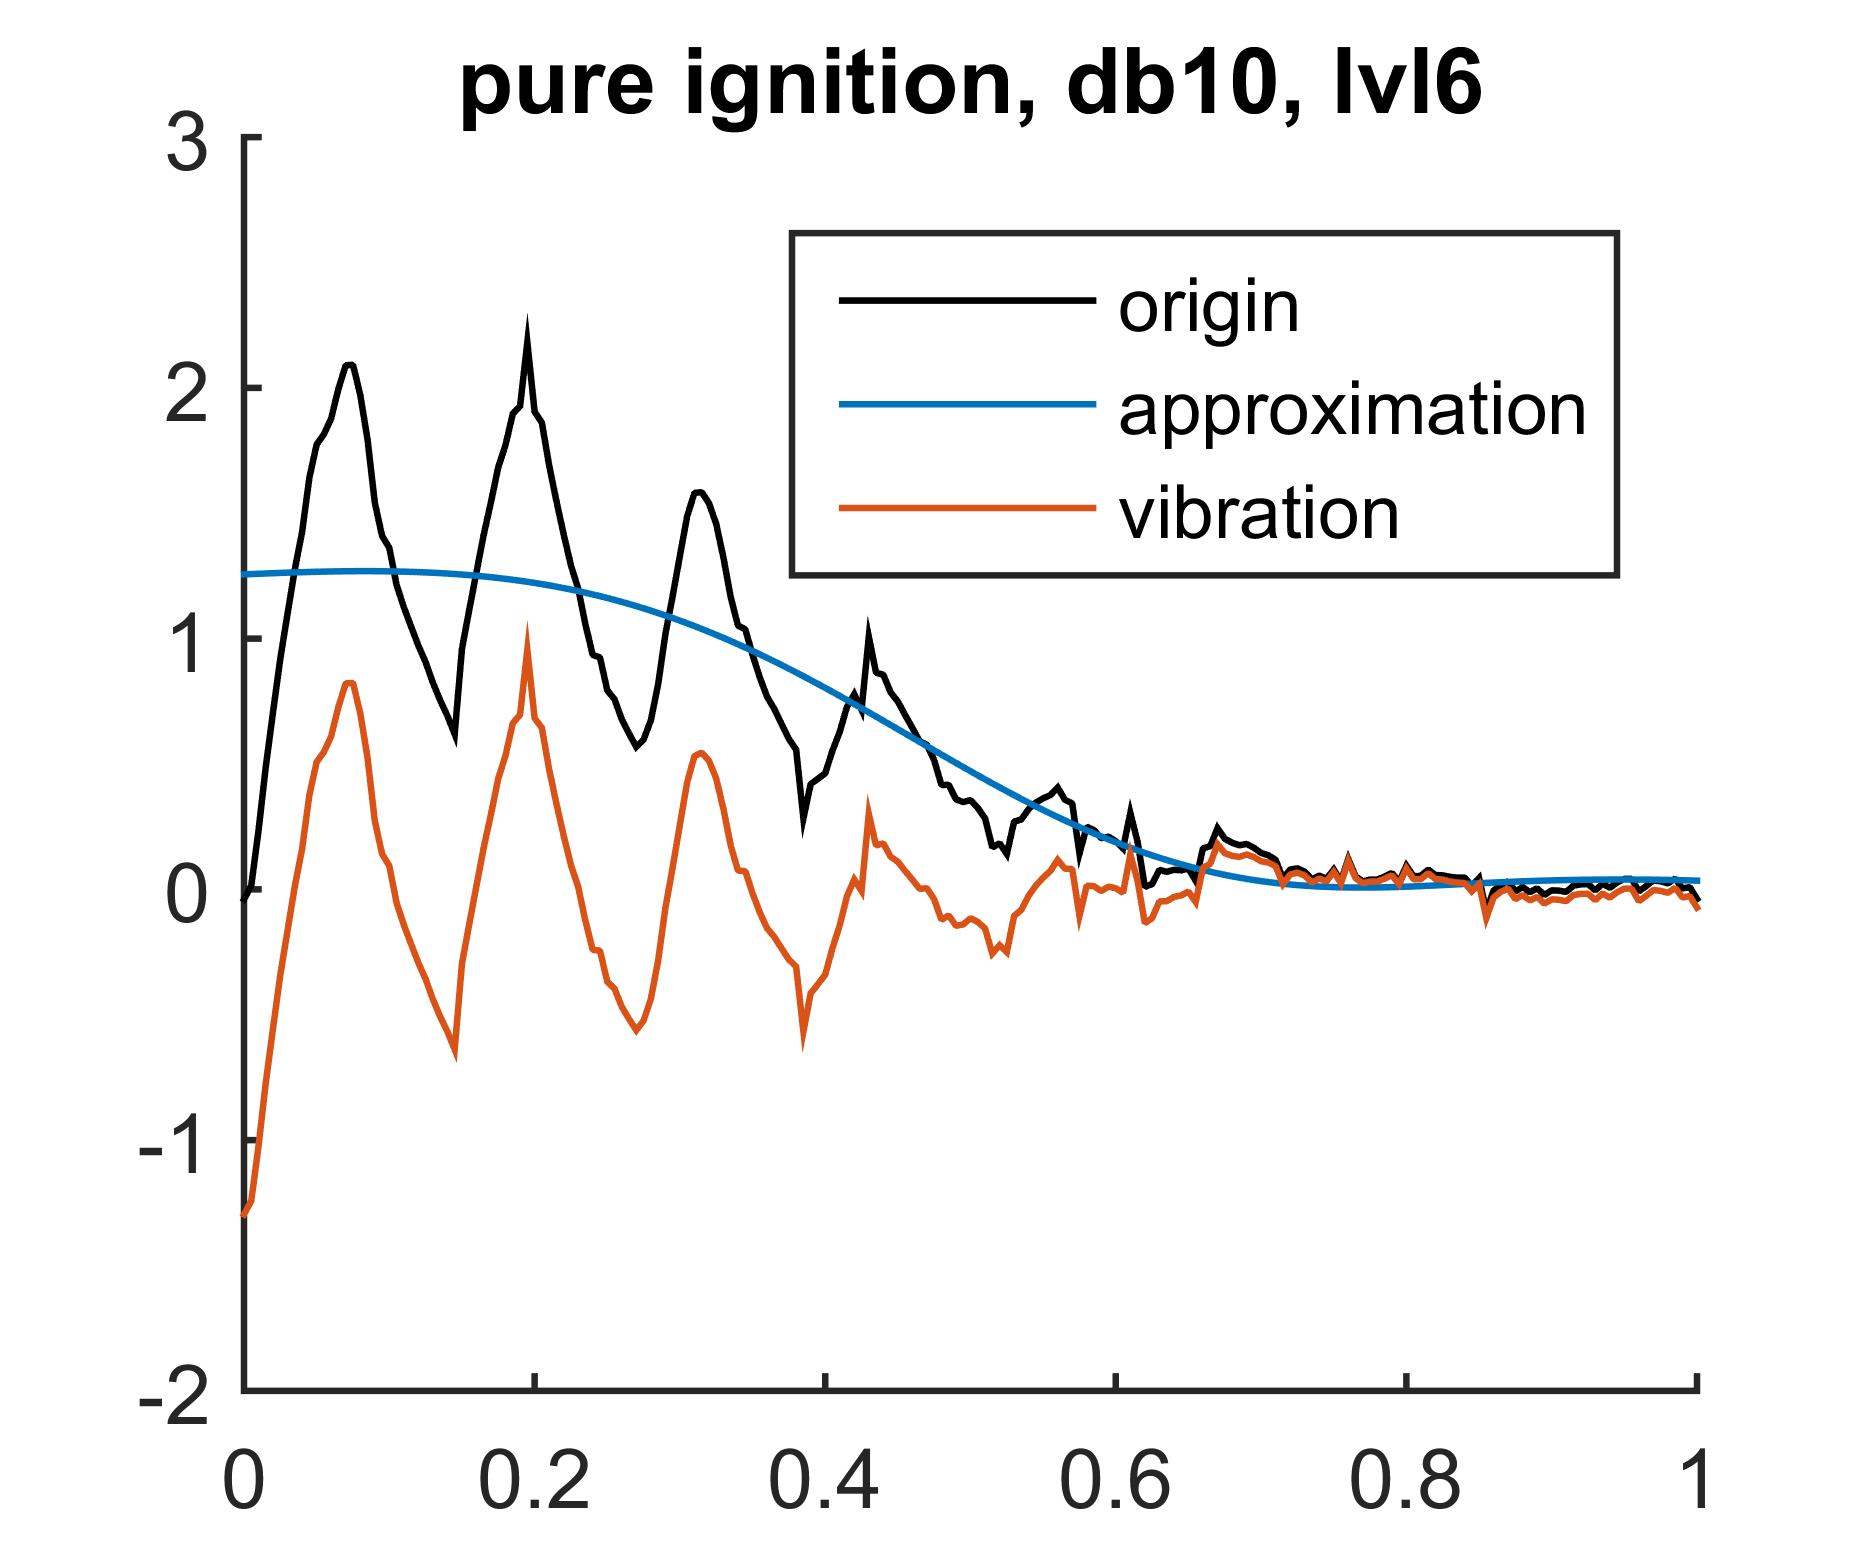
\includegraphics[width=0.3\textwidth]{thesis_figure/ion_chapter/db10_lvl6}&
		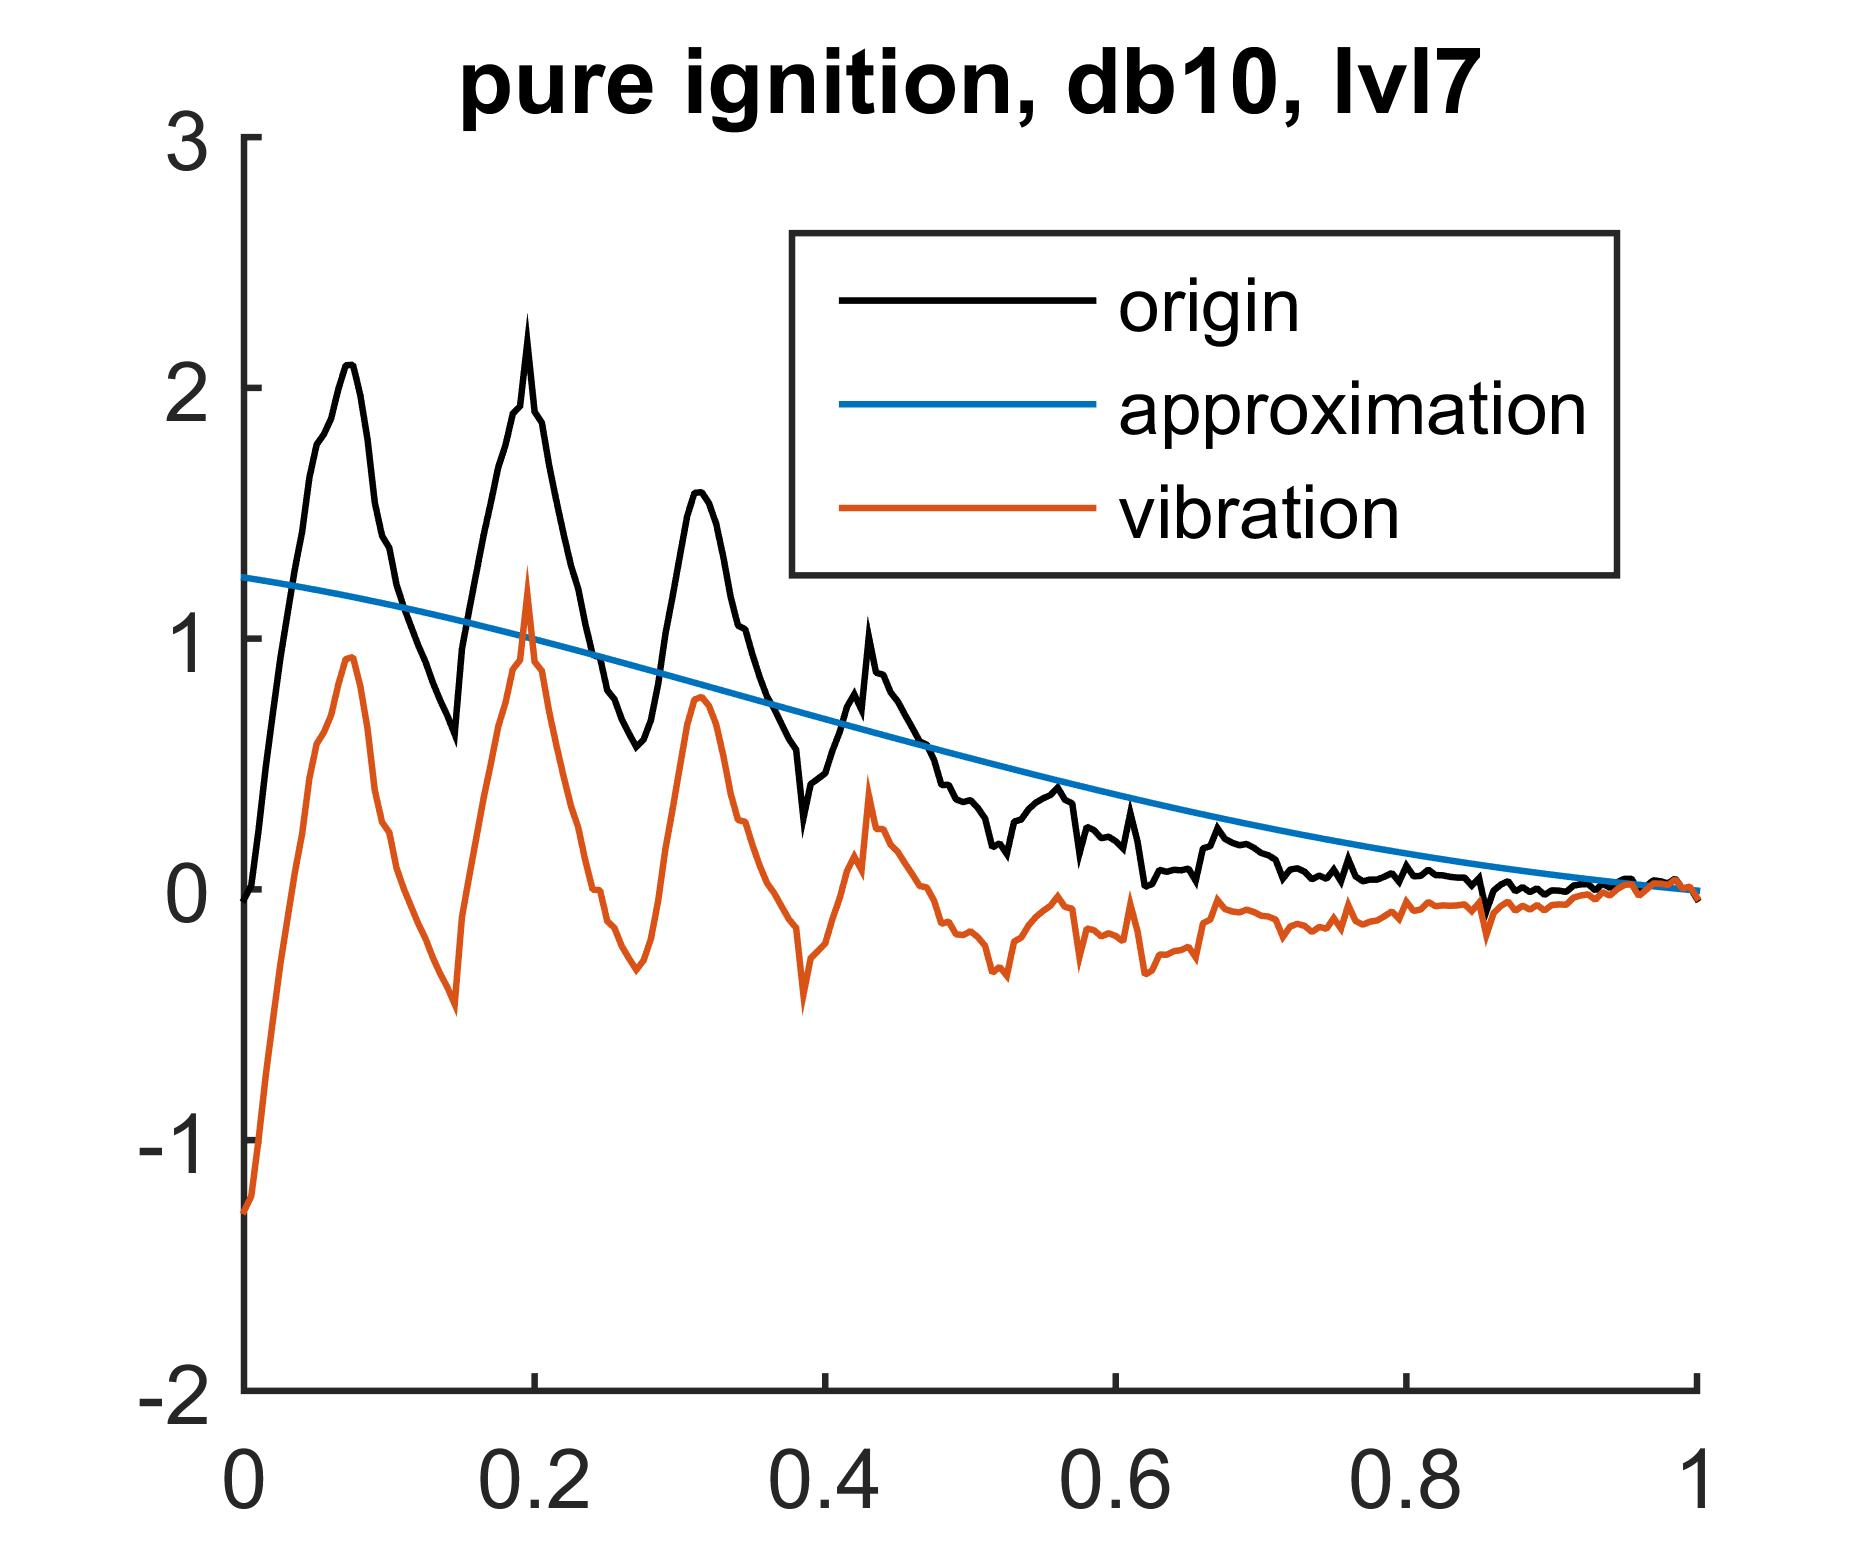
\includegraphics[width=0.3\textwidth]{thesis_figure/ion_chapter/db10_lvl7}
	\end{tabular}
	\caption{\label{fig:db10}db10小波对纯点火干扰信号进行10层分解}
\end{figure}
\par 先用db10小波对纯点火干扰信号进行10层分解,观察第二层到第七层的分解情况,如图\ref{fig:db10}所示,可以看到第二层和第三层并没有将震荡信号分解开来,而第六层和第七层分解出来的平滑信号过
于硬直,且分解的震荡信号不具有很好的衰减特性。而第四层分解相对于第五层分解来说,效果没有那么理想。所以本文以下的小波分析都是基于第五层分解来进行的。由于dmey没有阶数问题,而coif小波
的最高阶数为5。所以只讨论db小波和sym小波的阶数问题。
\subsection{db小波族的阶数选择和分析}
取阶数分别为5、10、15、20、25和30的db小波对纯干扰信号进行分析。
\begin{figure}[!htb]
	\centering
	\begin{tabular}{ccc}
		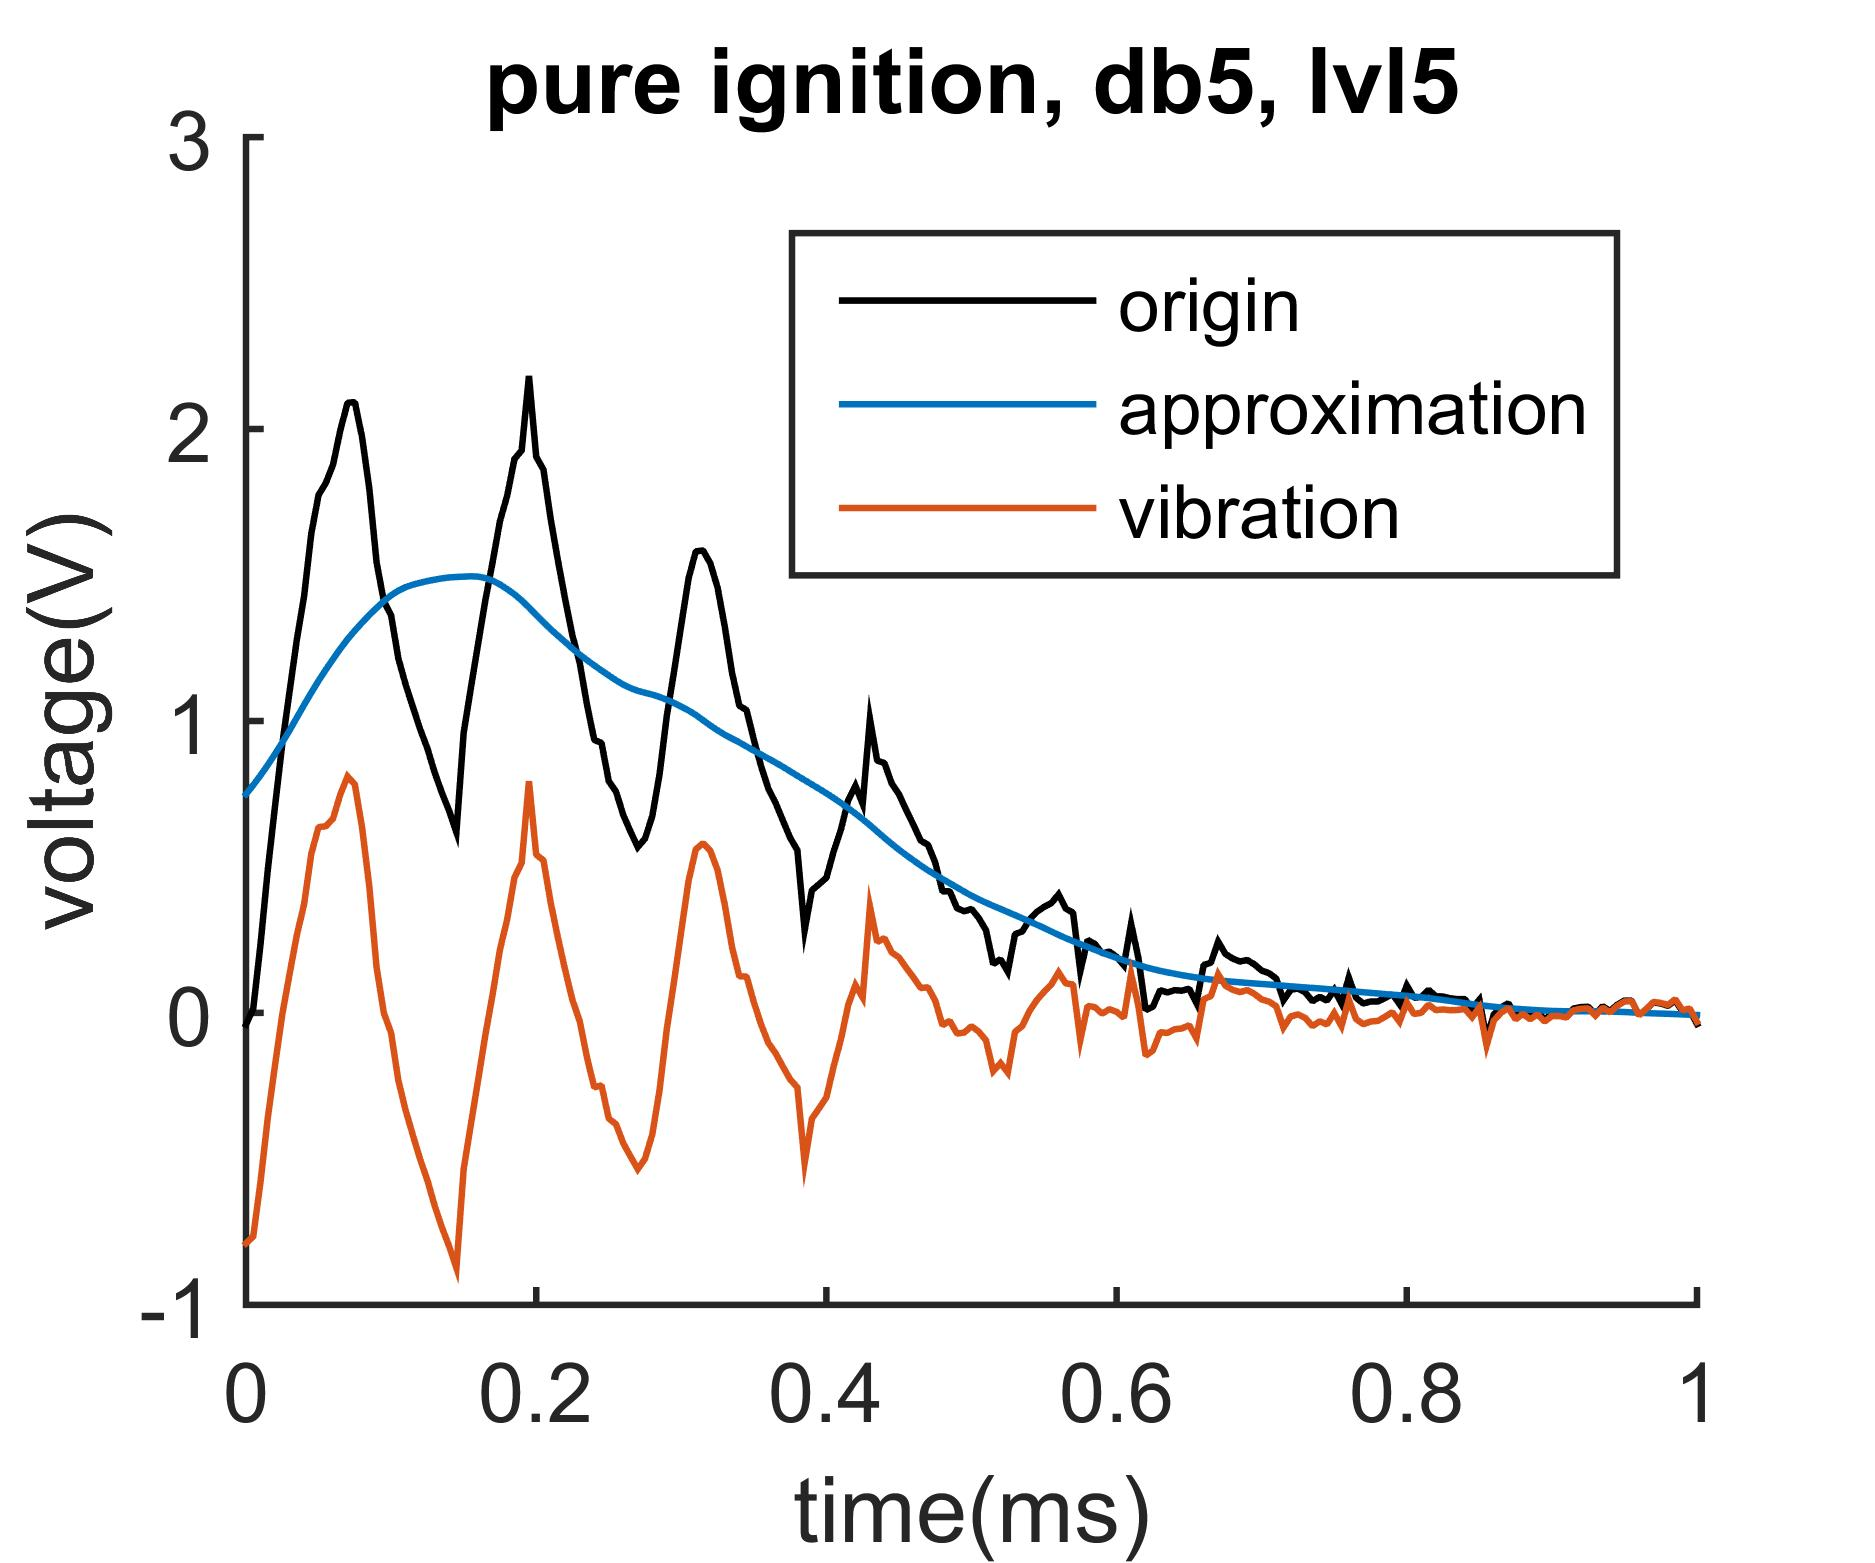
\includegraphics[width=0.3\textwidth]{thesis_figure/ion_chapter/db5_lvl5}&
		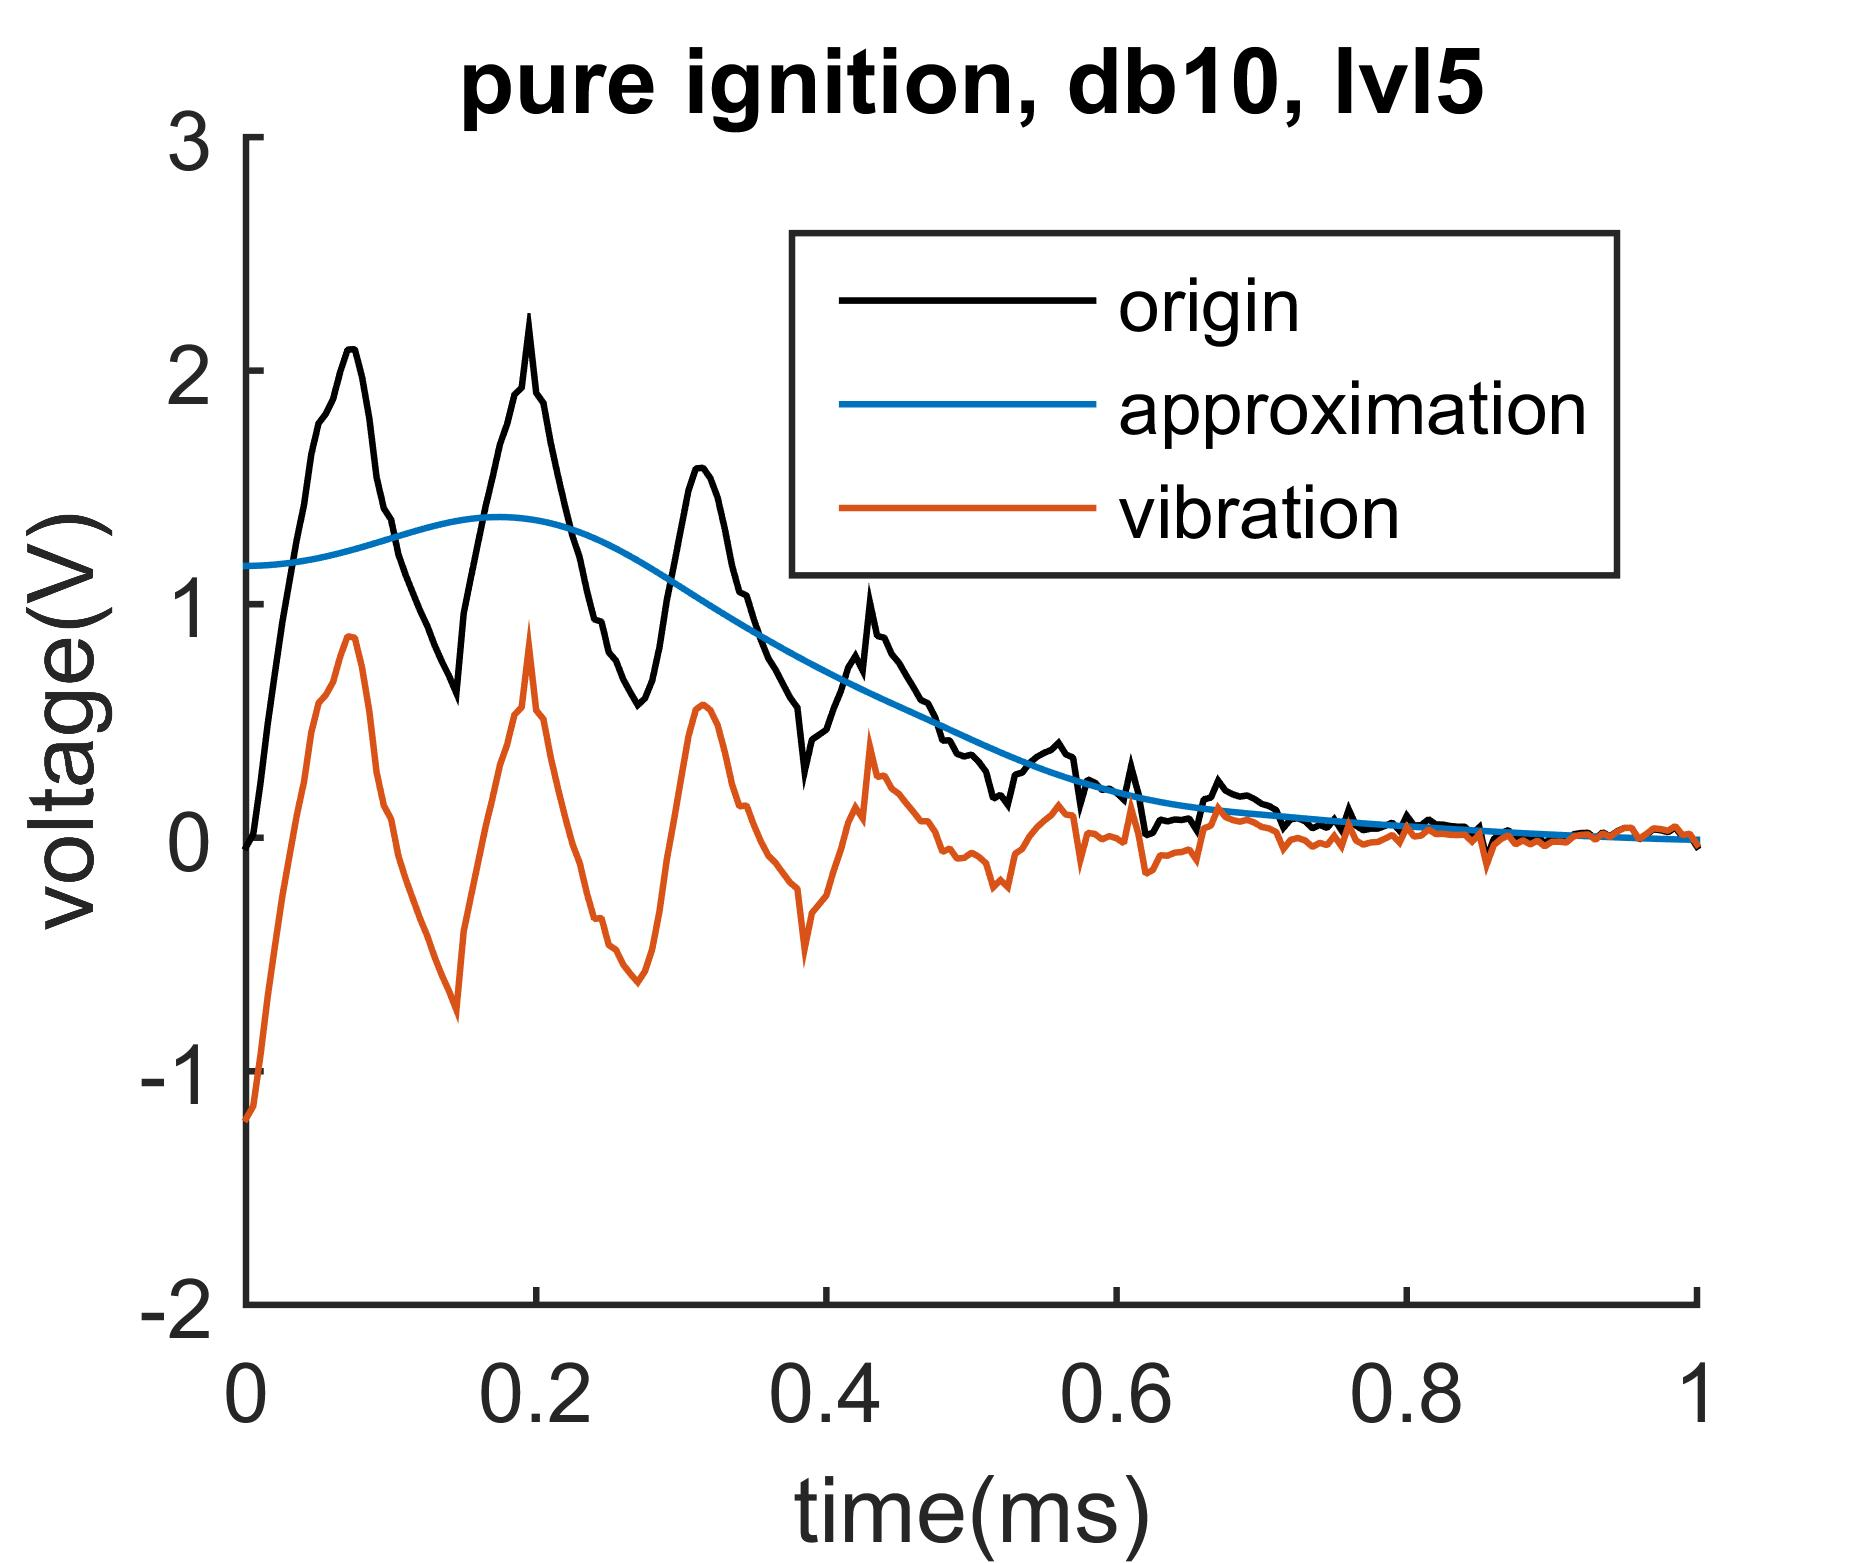
\includegraphics[width=0.3\textwidth]{thesis_figure/ion_chapter/db10_lvl5_1}&
		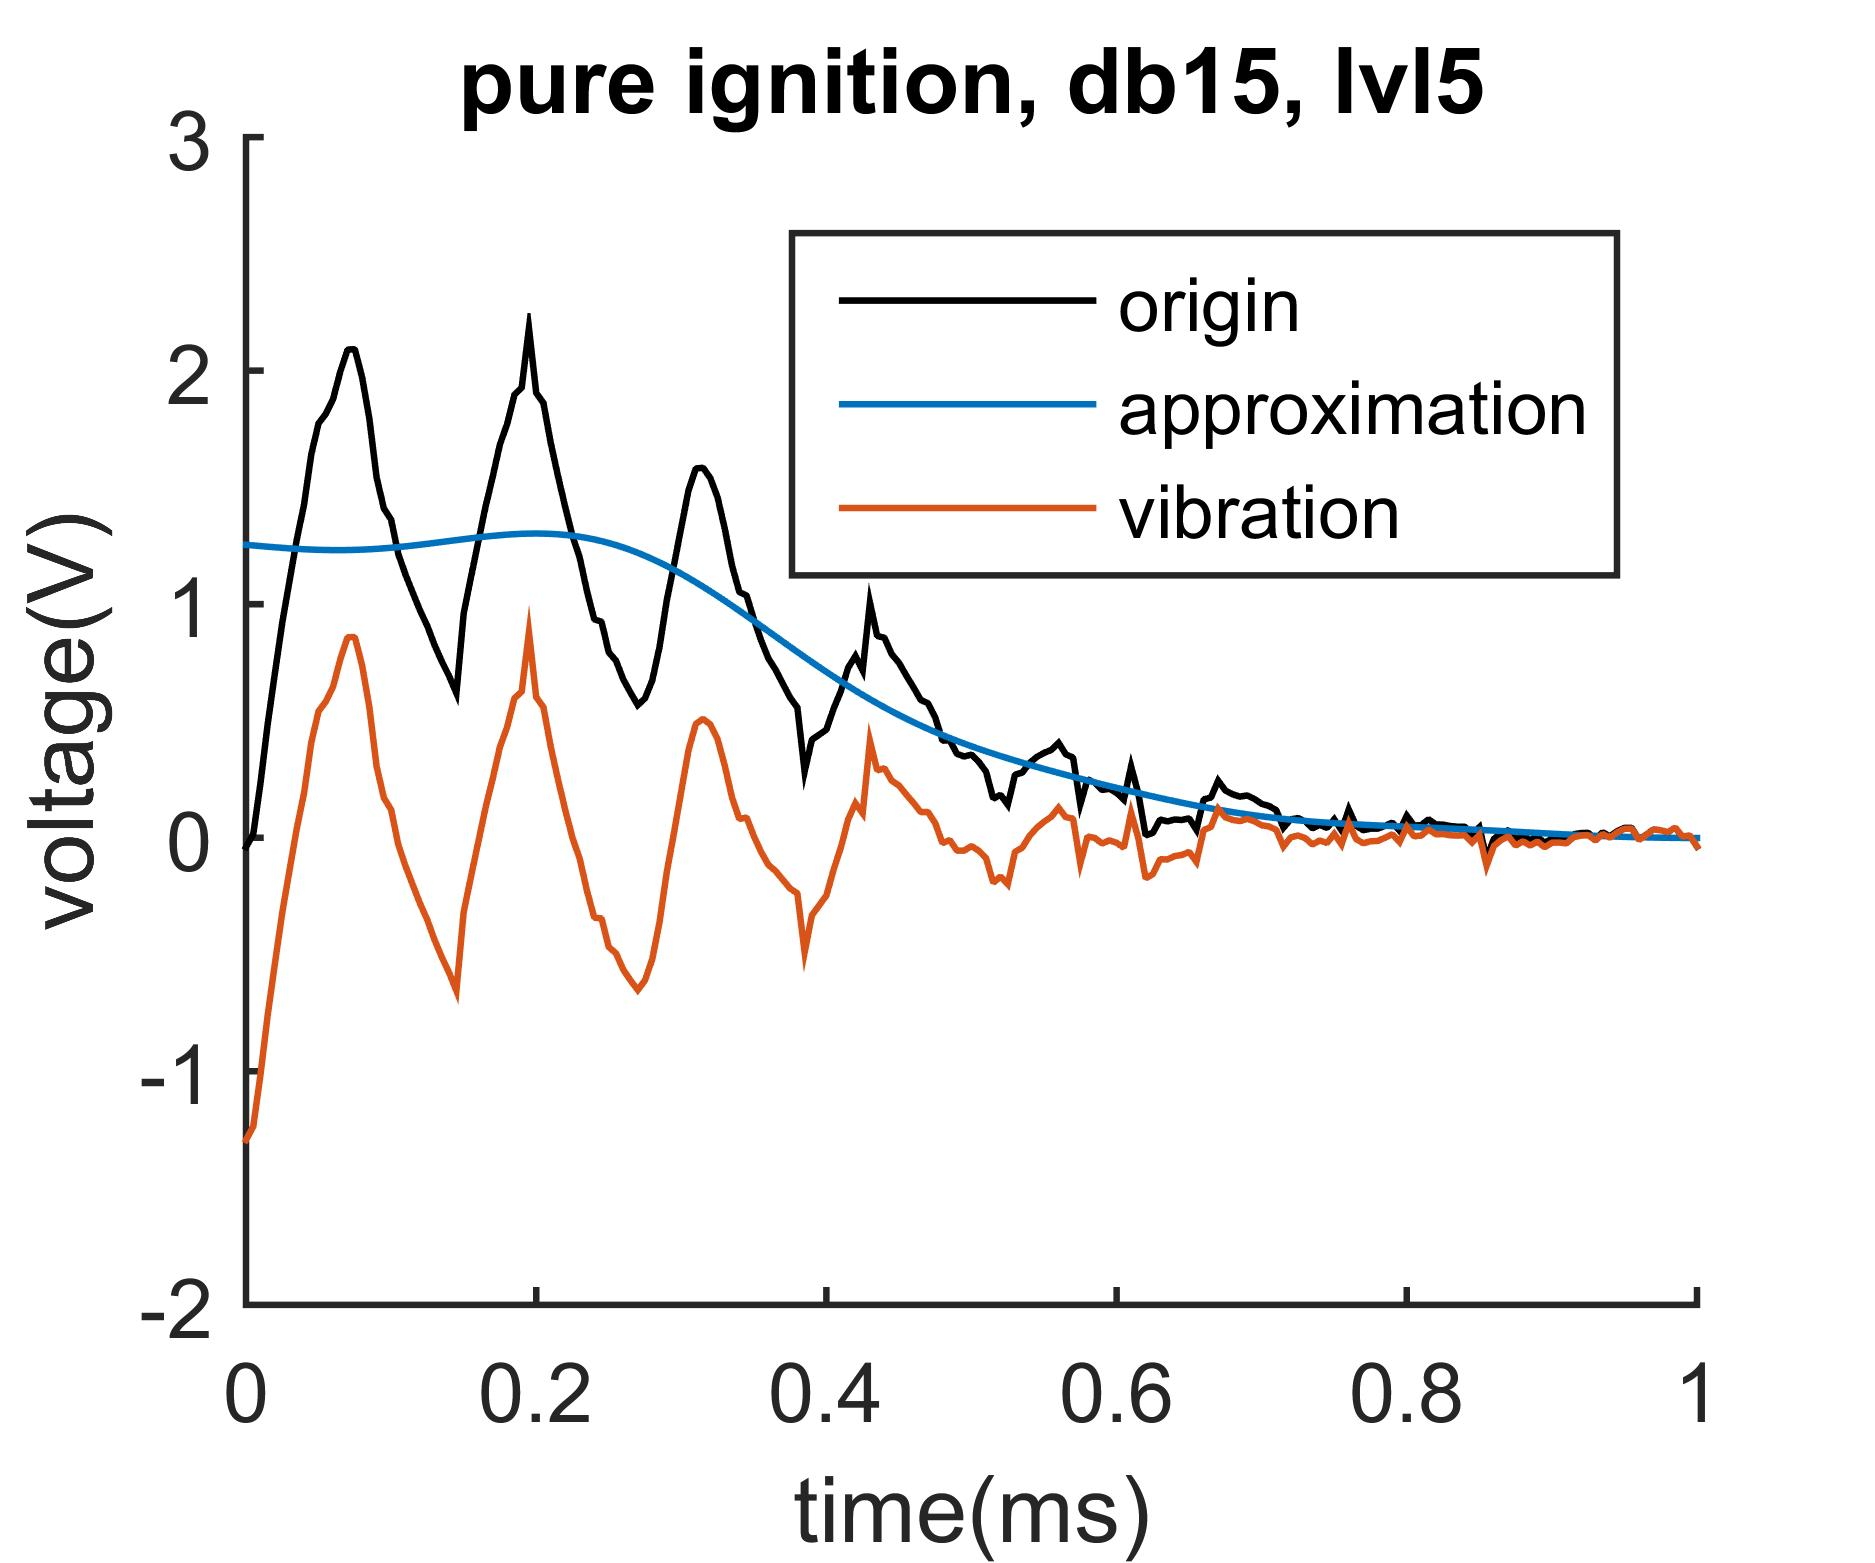
\includegraphics[width=0.3\textwidth]{thesis_figure/ion_chapter/db15_lvl5}\\
		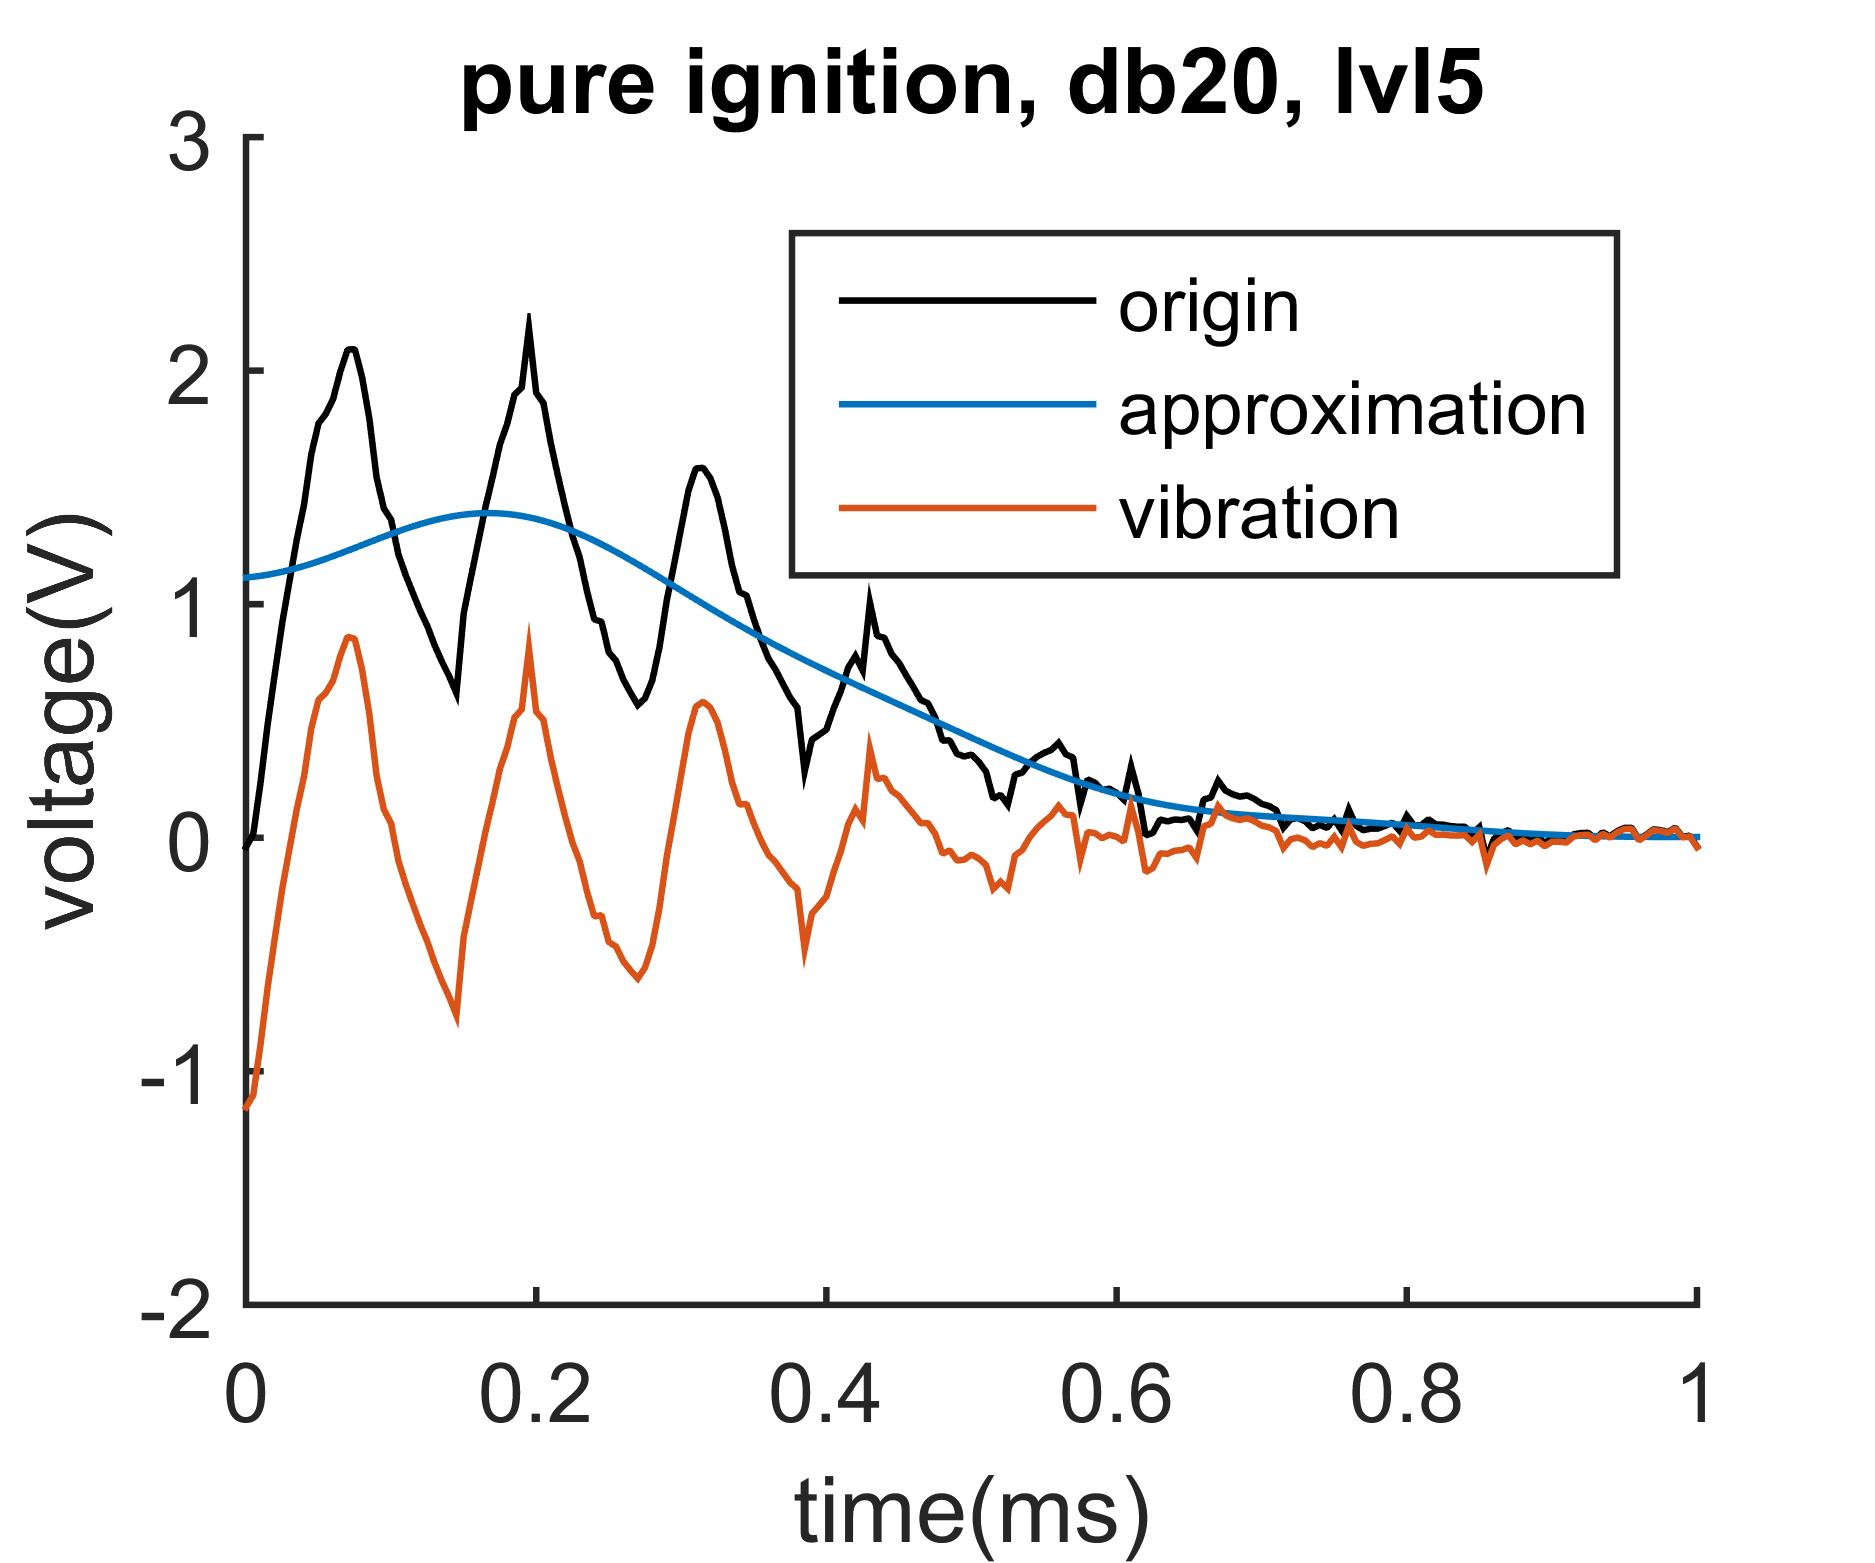
\includegraphics[width=0.3\textwidth]{thesis_figure/ion_chapter/db20_lvl5}&
		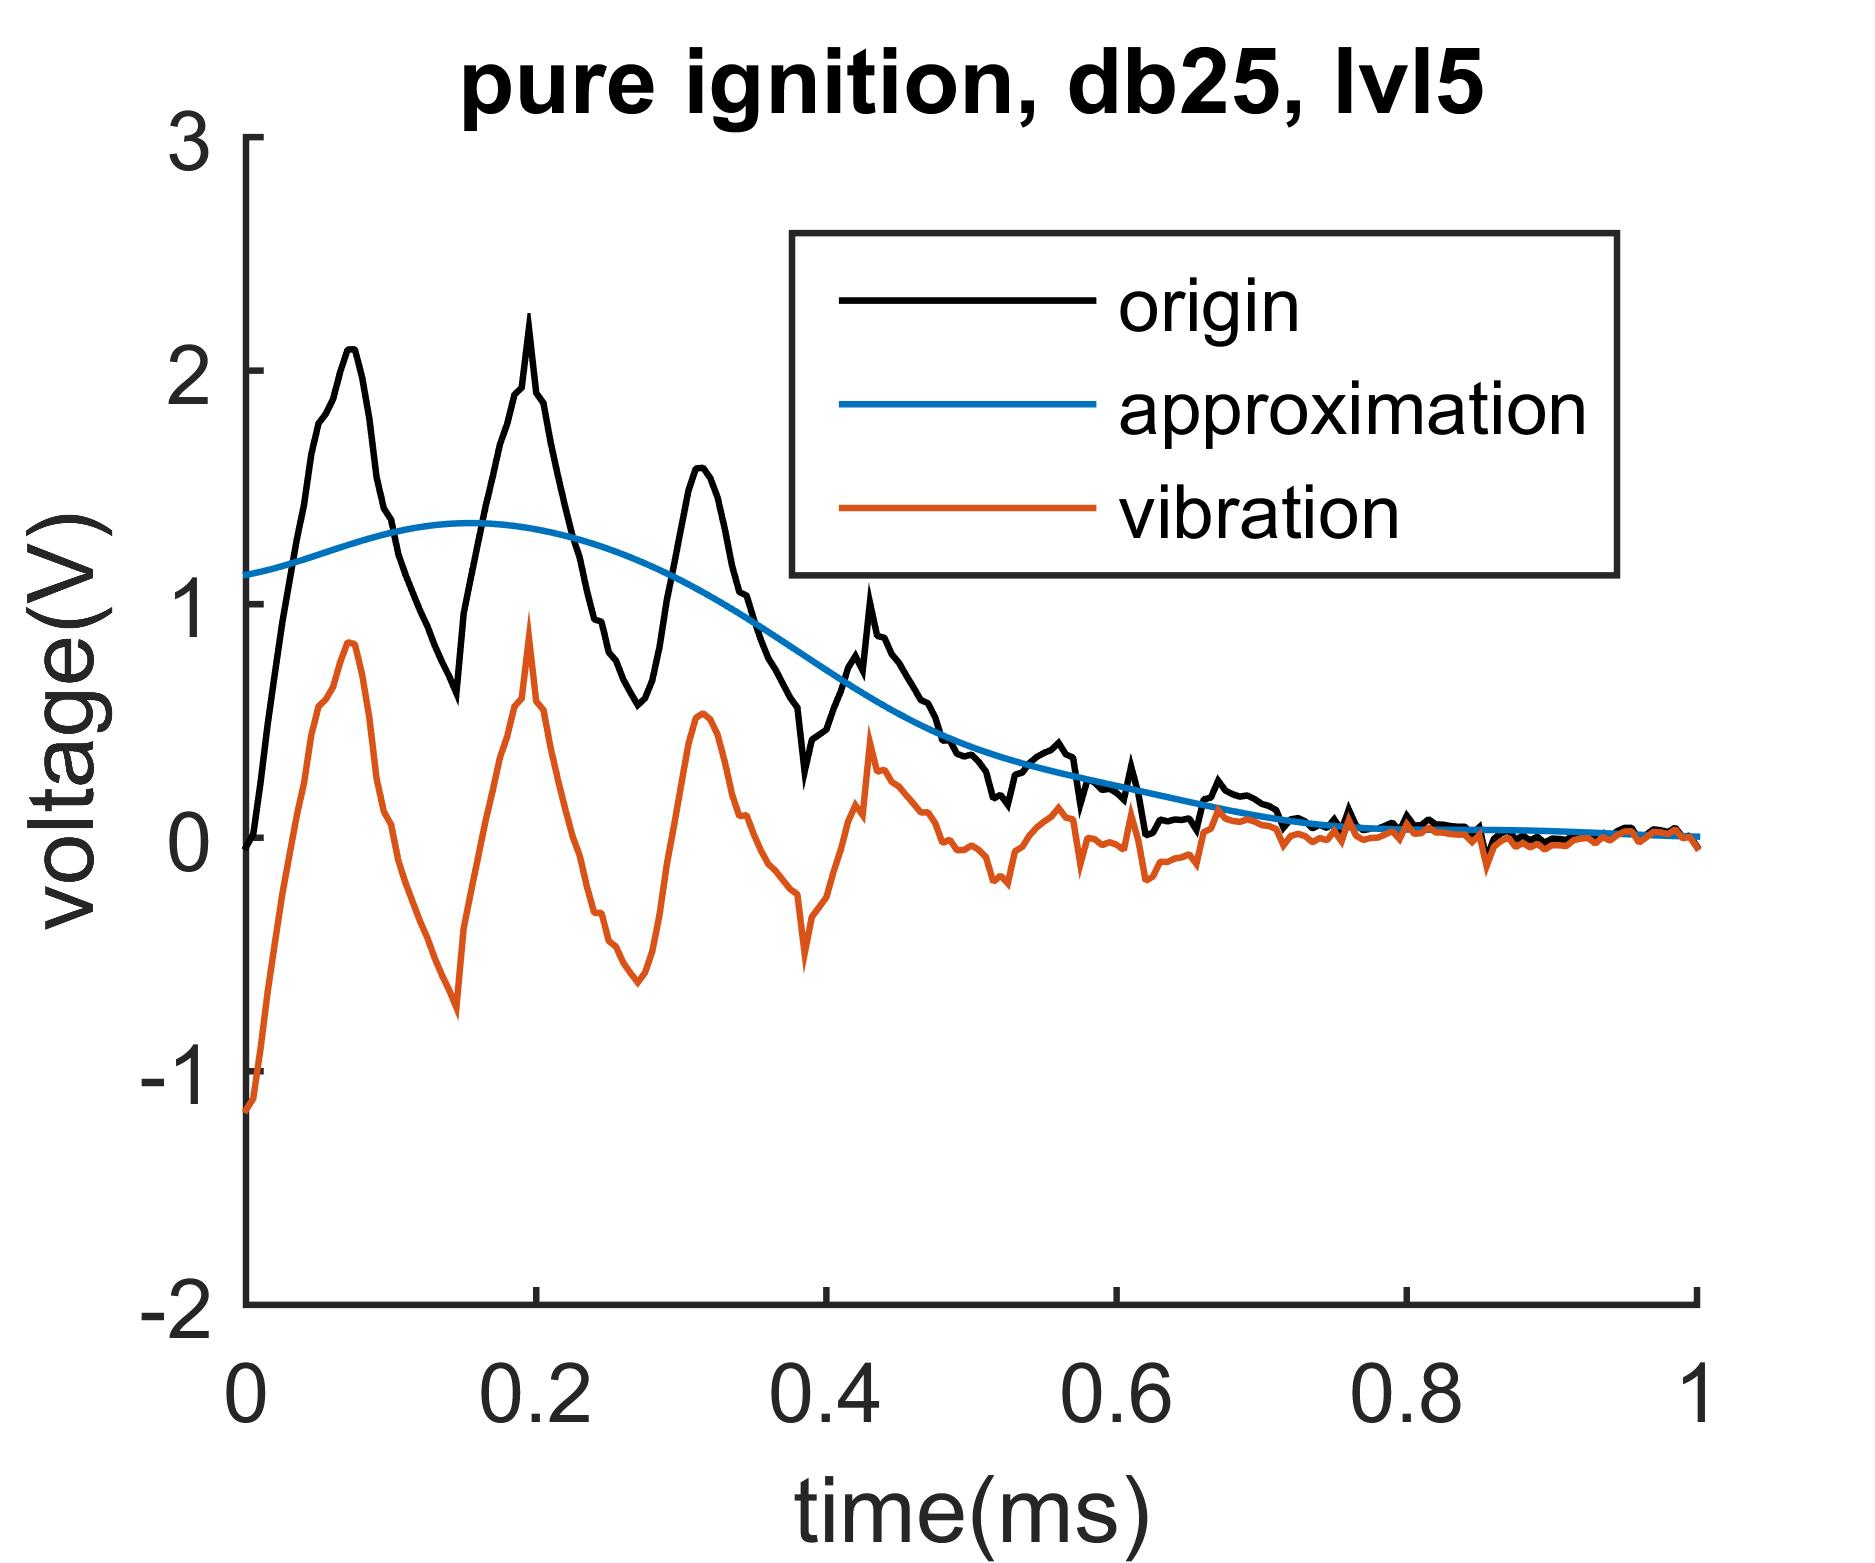
\includegraphics[width=0.3\textwidth]{thesis_figure/ion_chapter/db25_lvl5}&
		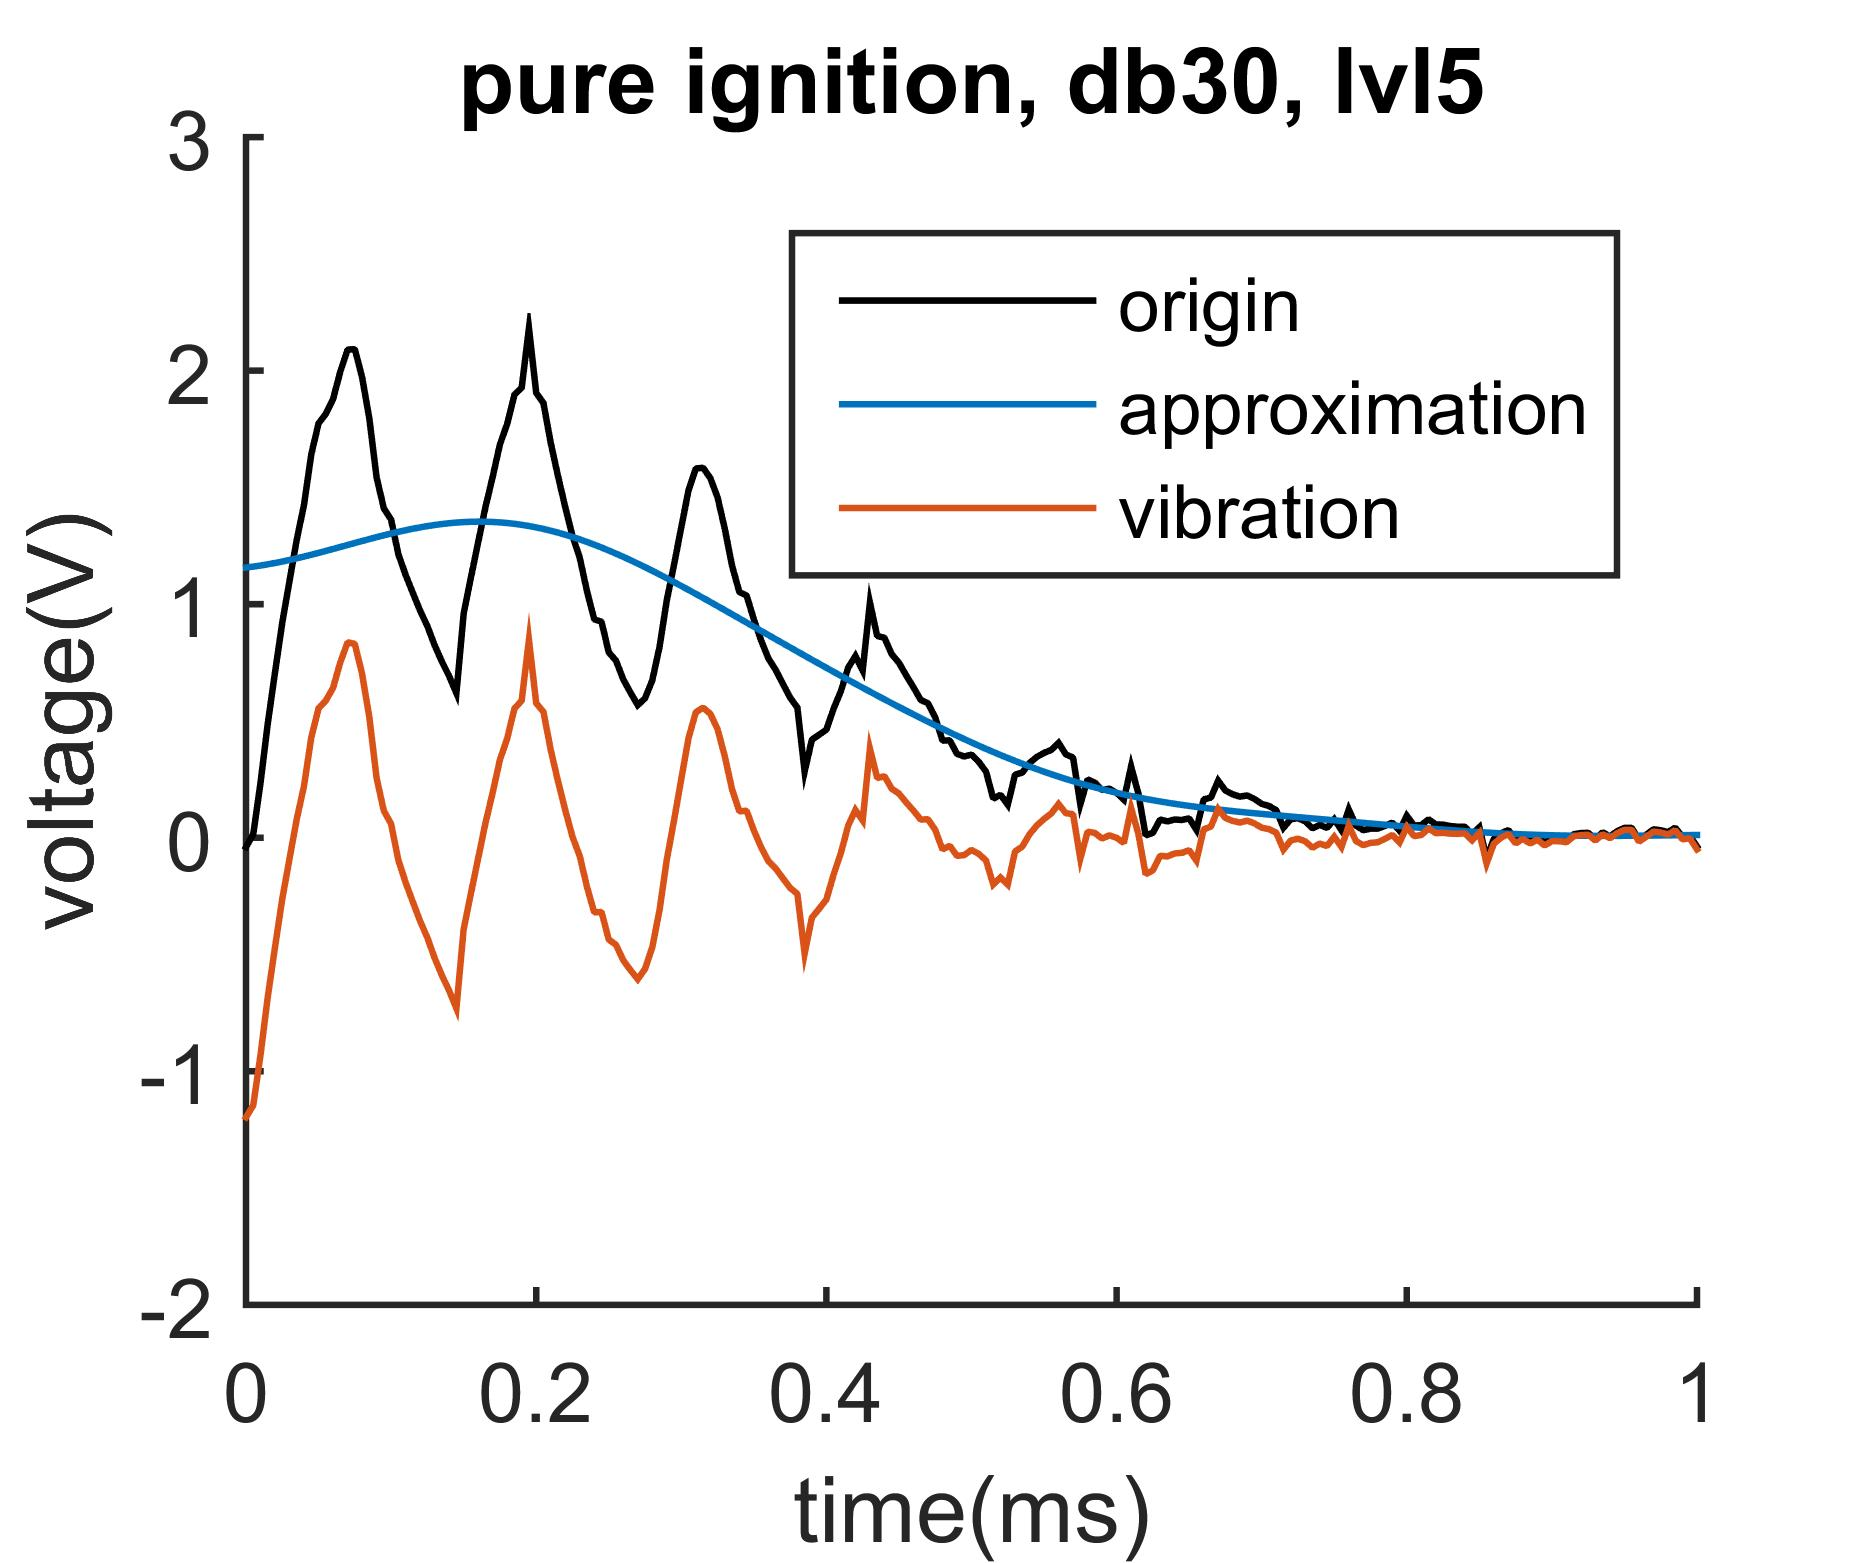
\includegraphics[width=0.3\textwidth]{thesis_figure/ion_chapter/db30_lvl5}
	\end{tabular}
	\caption{\label{fig:dbvar}不同阶数下的db小波第五层分解}
\end{figure}
从图\ref{fig:dbvar}中可以看到当阶数增加后,小波第五层分解的结果不变,考虑到分解阶数越多计算越加复杂。则取db20作为db小波分解的小波函数。
\subsection{sym小波族的阶数选择和分析}
\begin{figure}[H]
	\centering
	\begin{tabular}{ccc}
		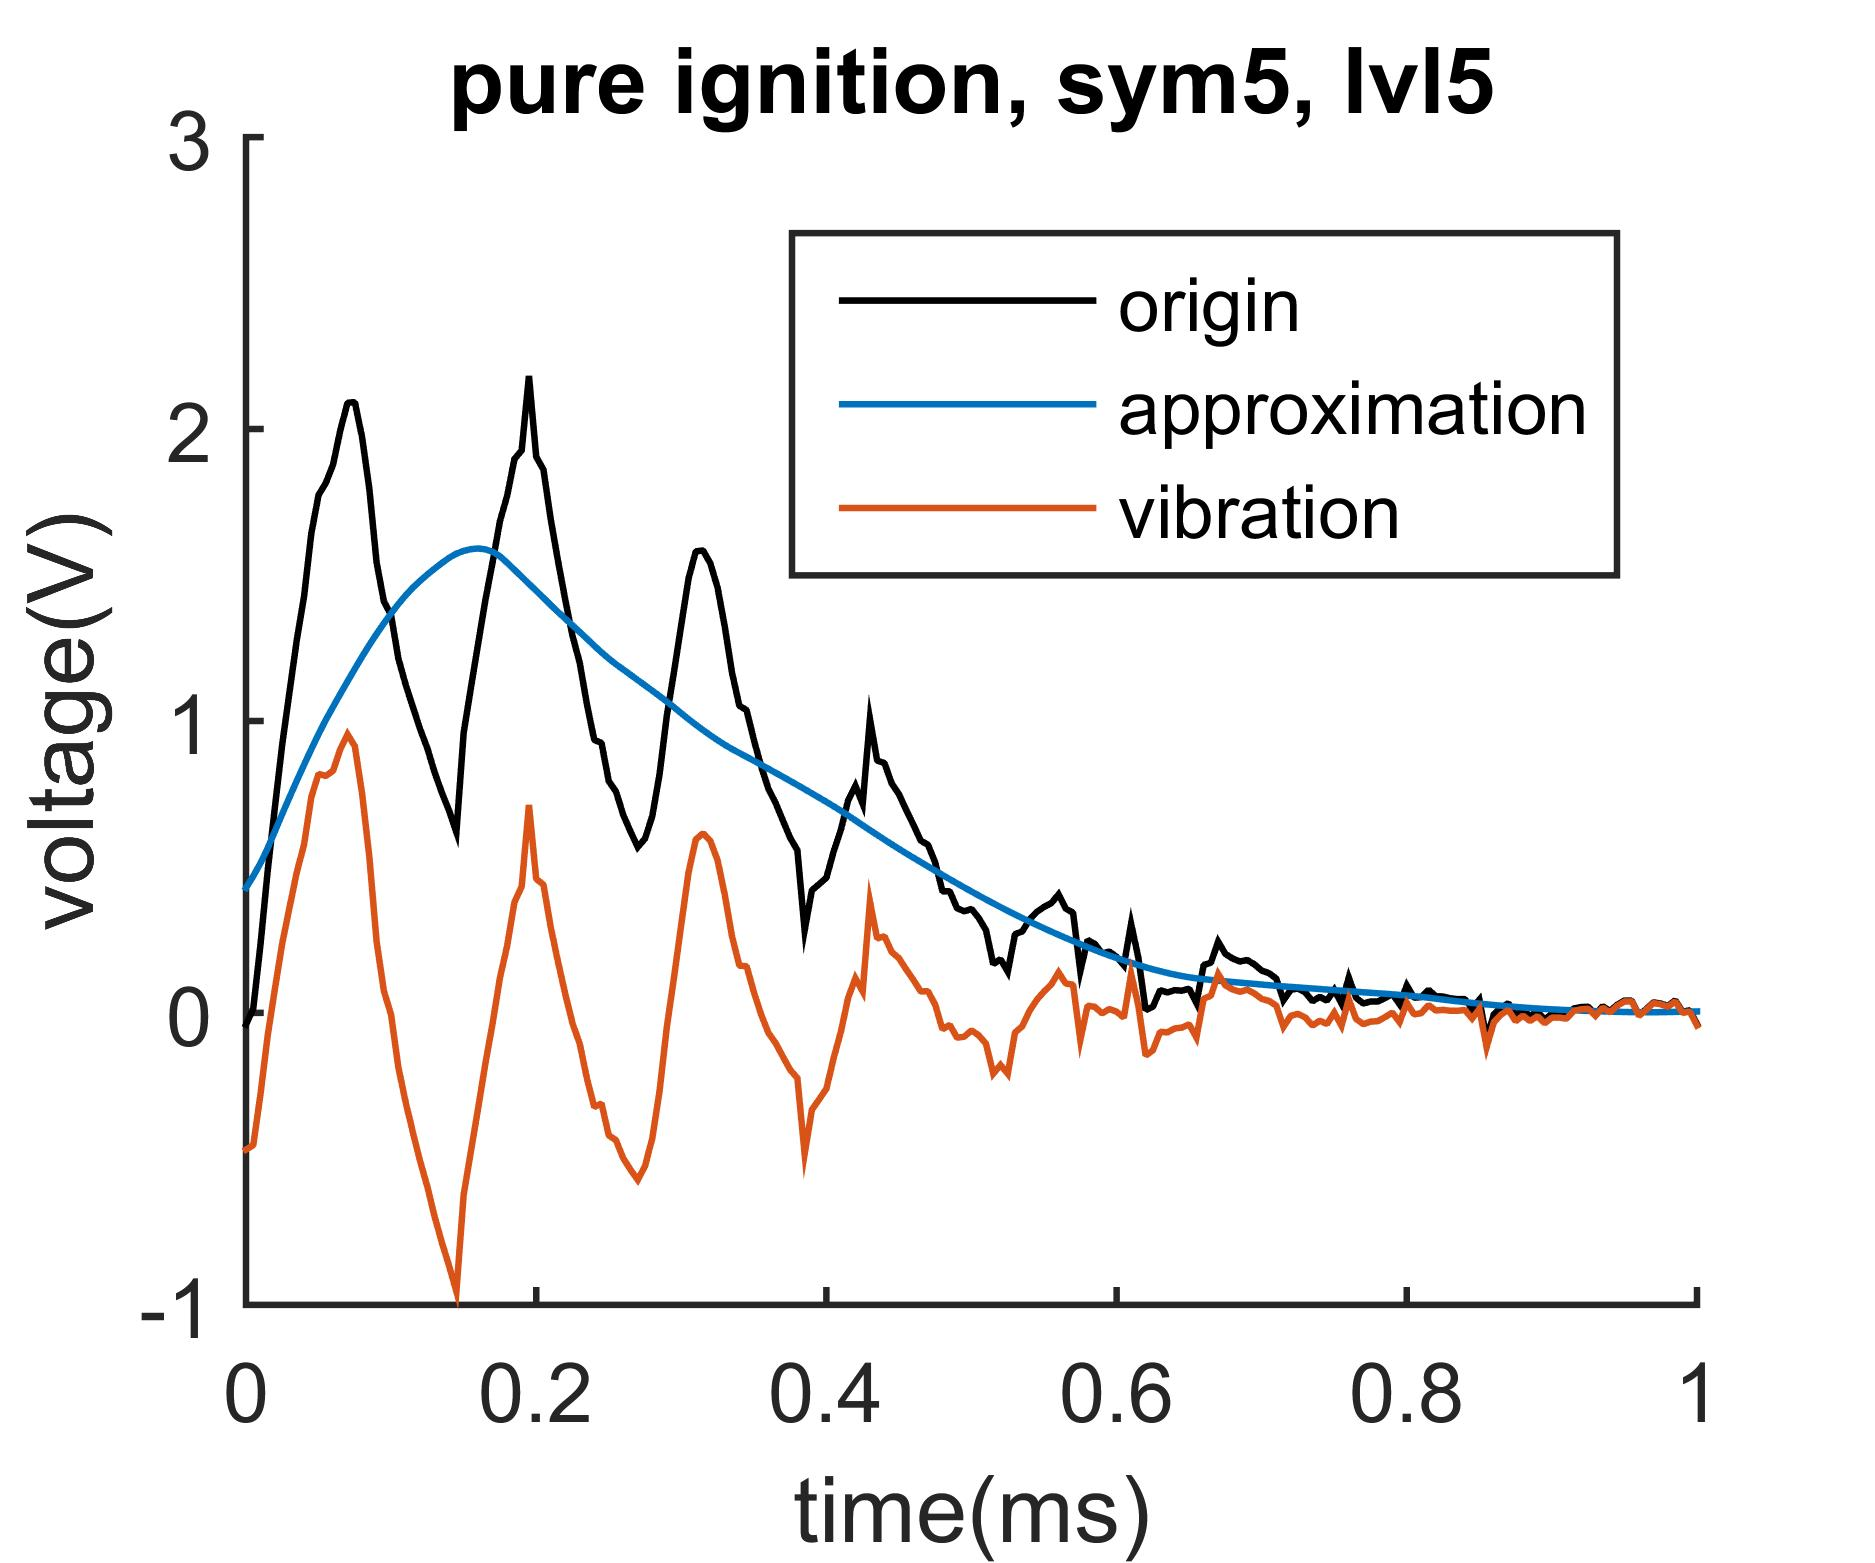
\includegraphics[width=0.3\textwidth]{thesis_figure/ion_chapter/sym5_lvl5}&
		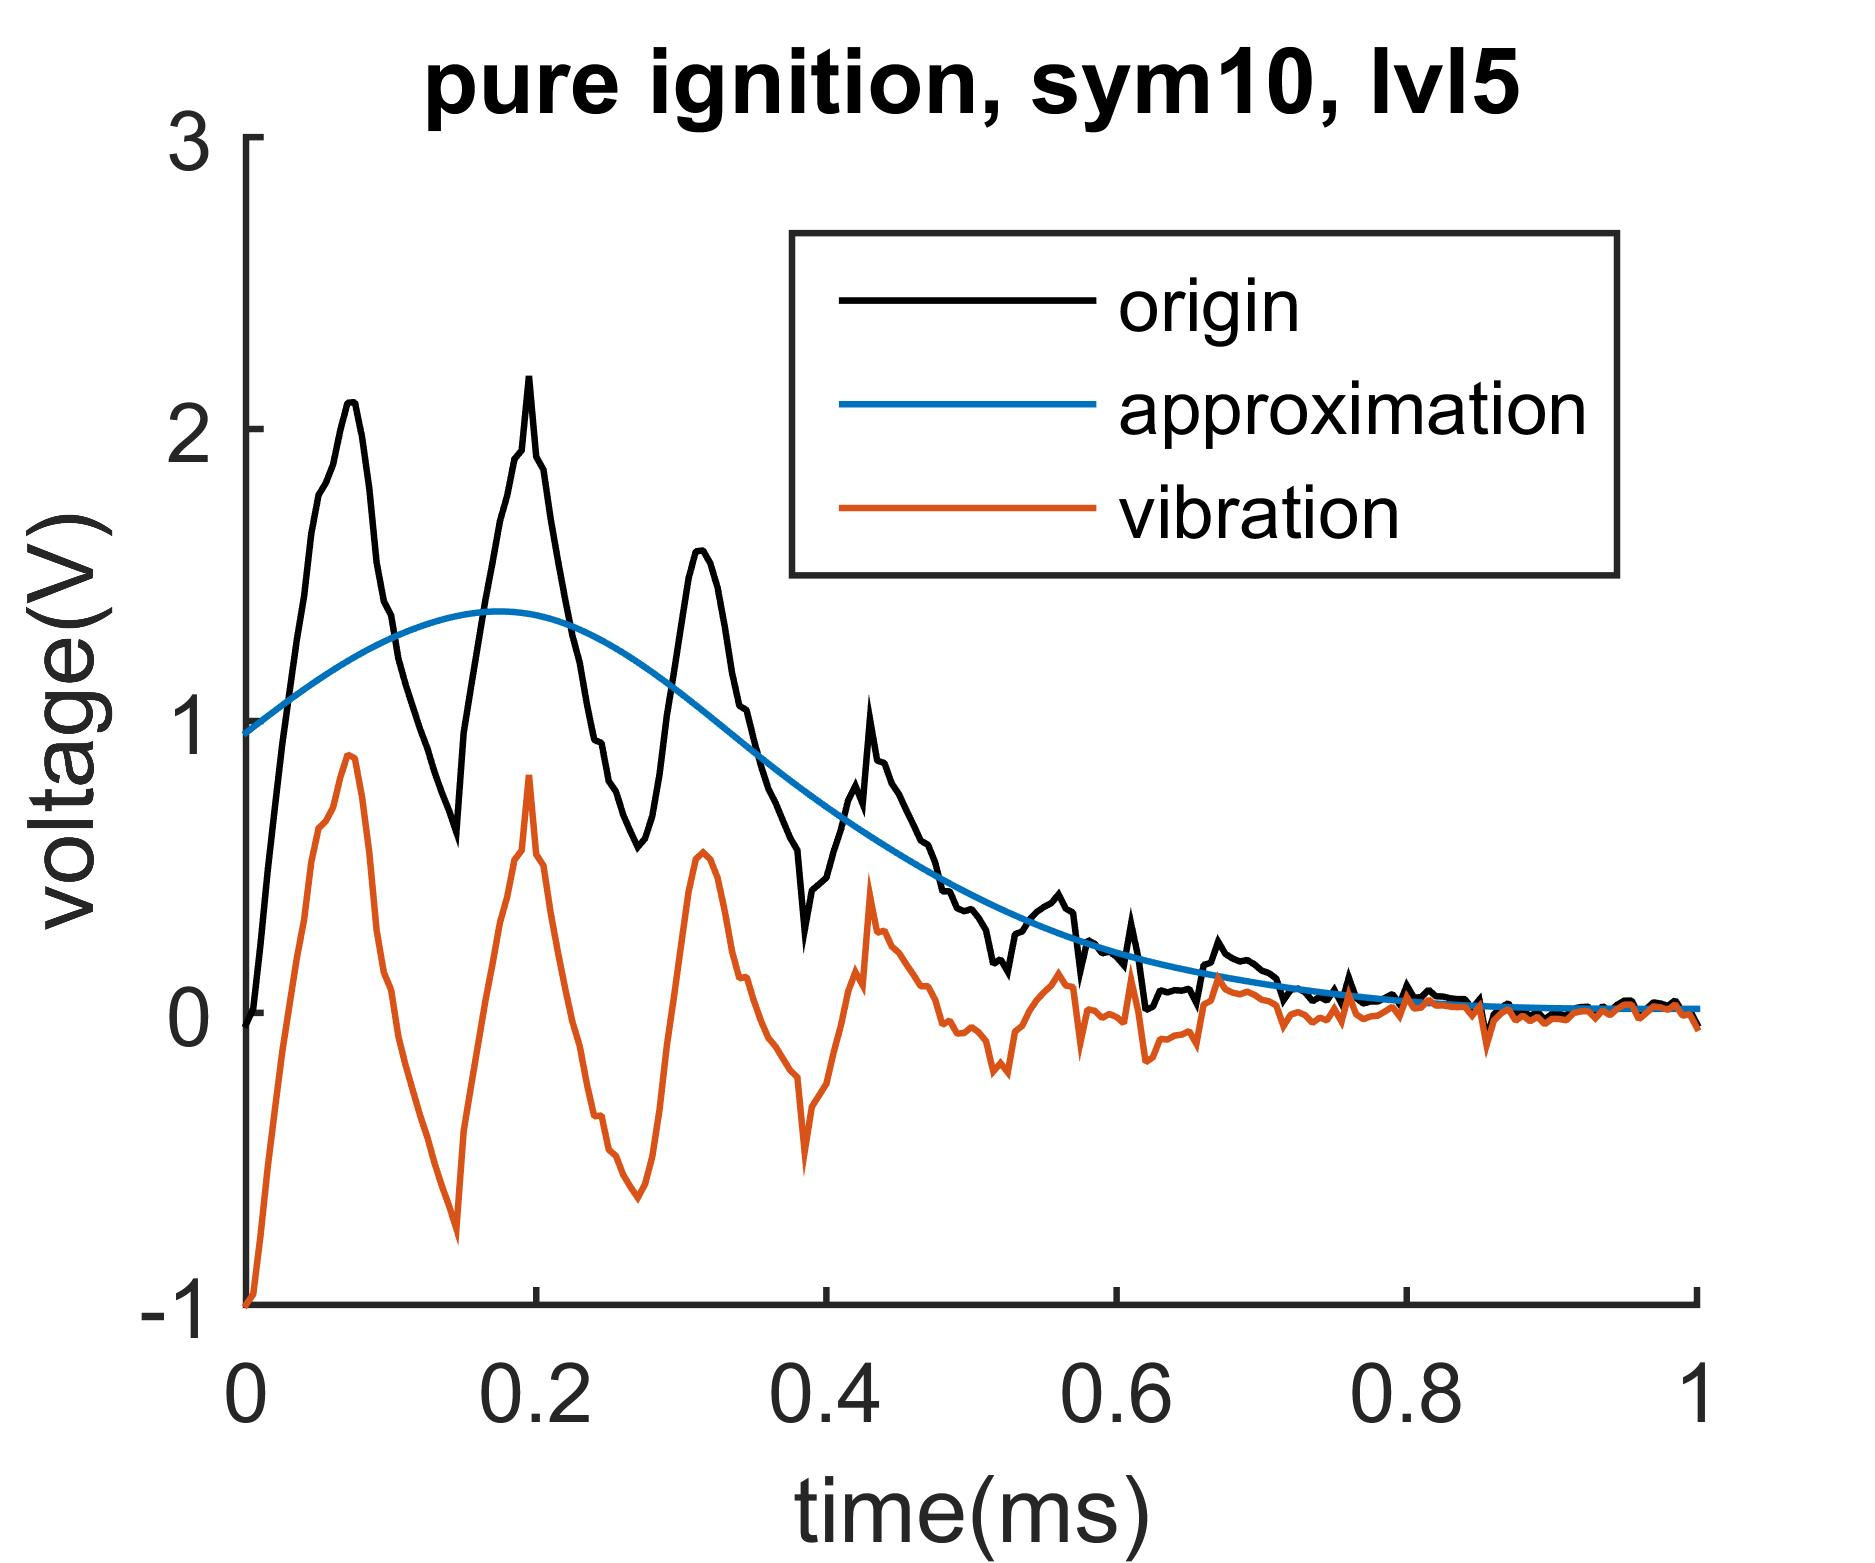
\includegraphics[width=0.3\textwidth]{thesis_figure/ion_chapter/sym10_lvl5}&
		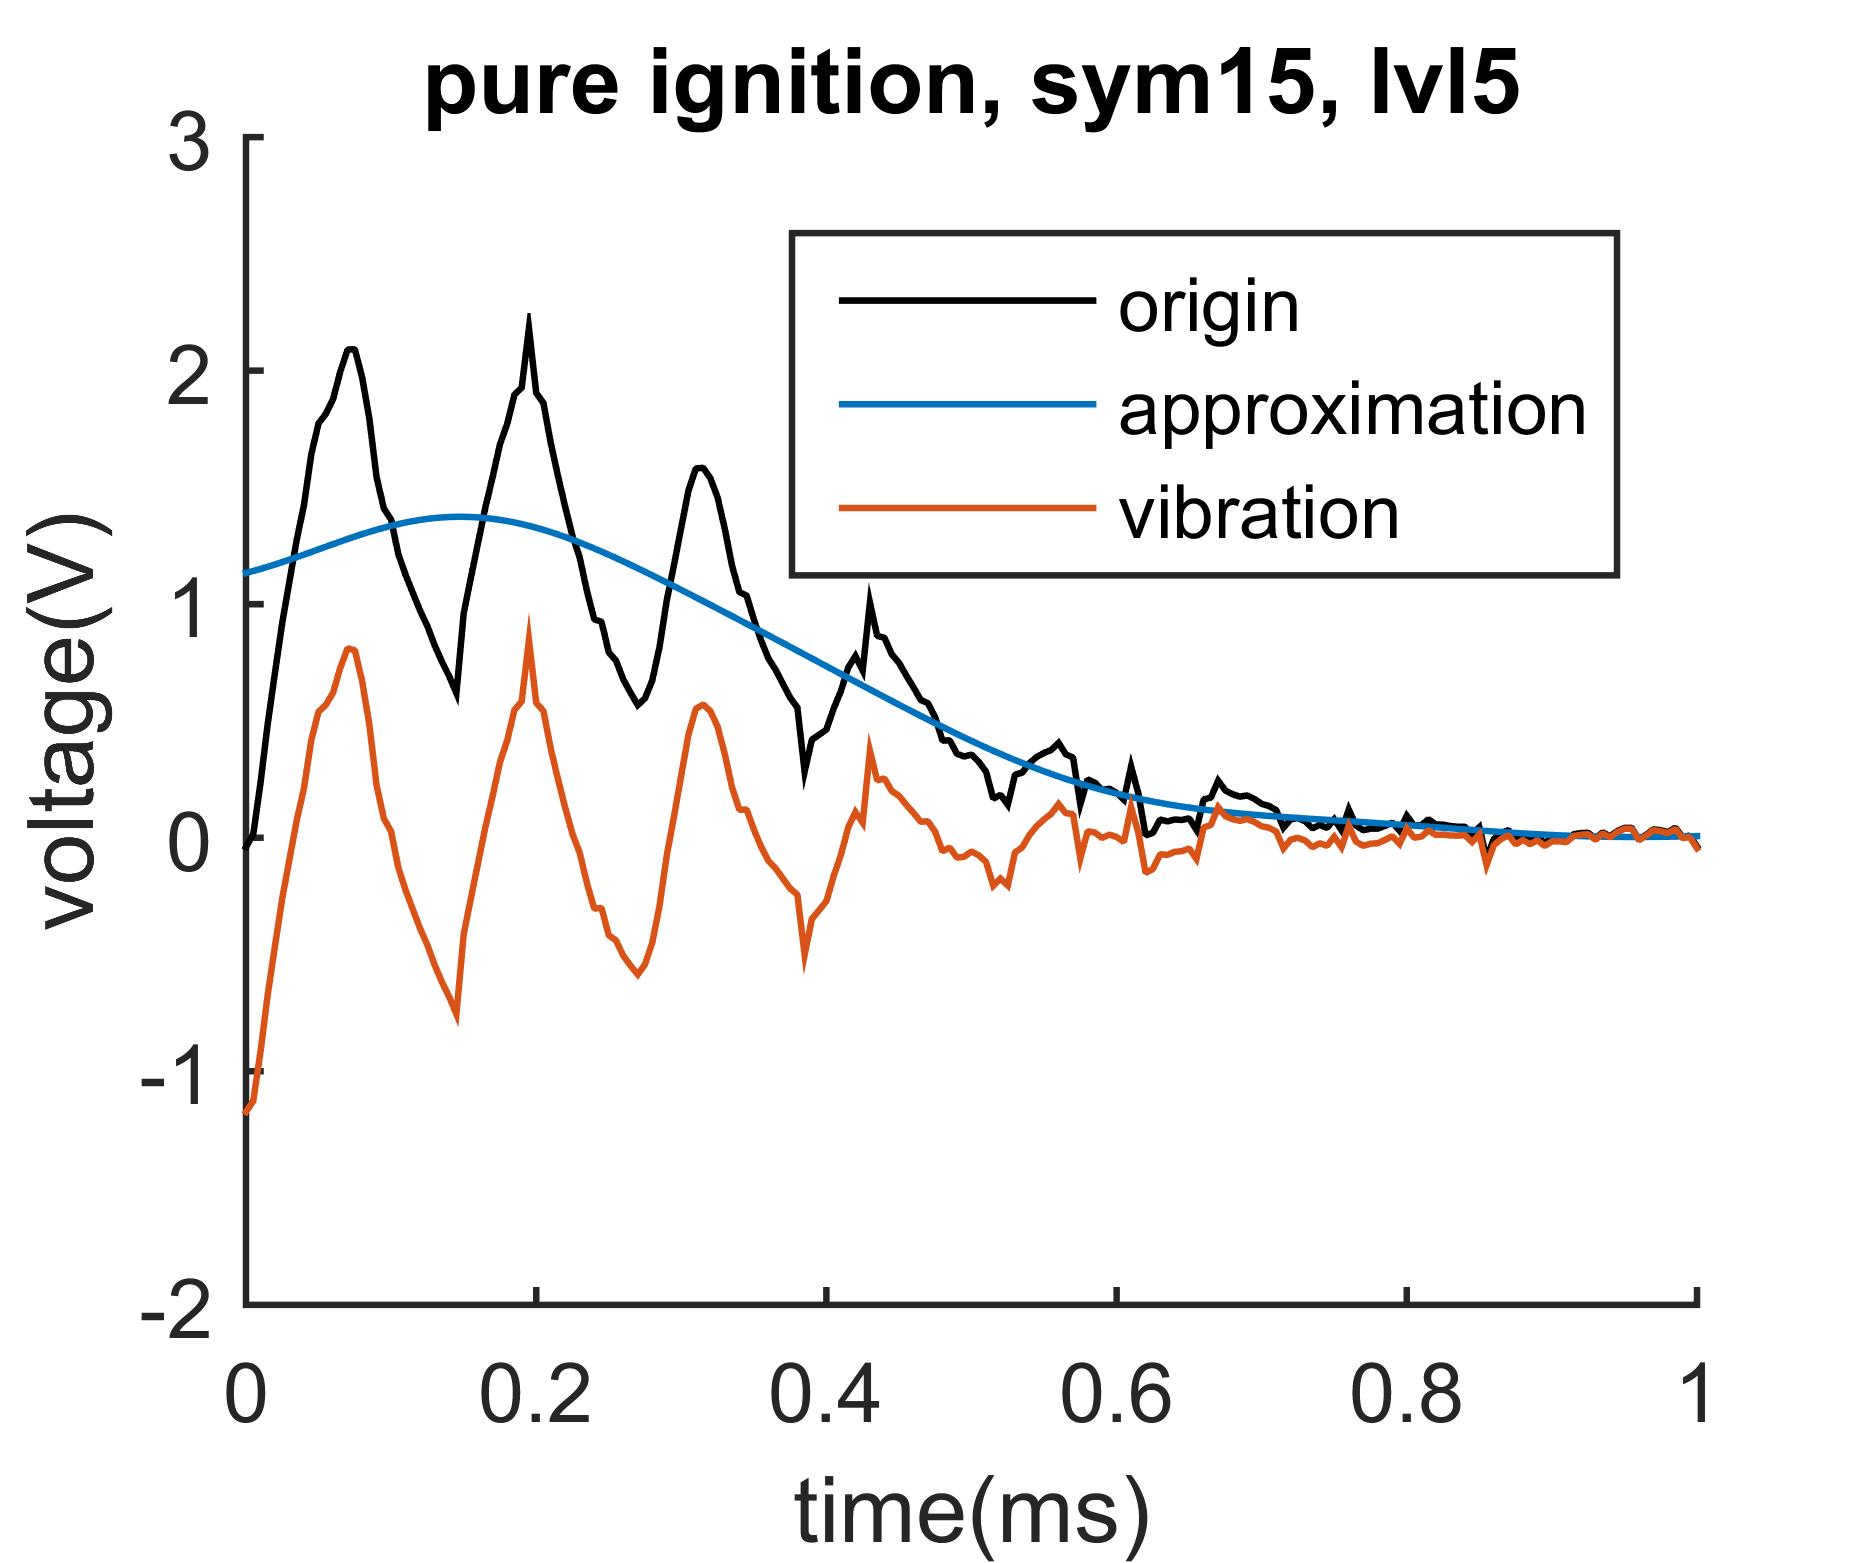
\includegraphics[width=0.3\textwidth]{thesis_figure/ion_chapter/sym15_lvl5}\\
		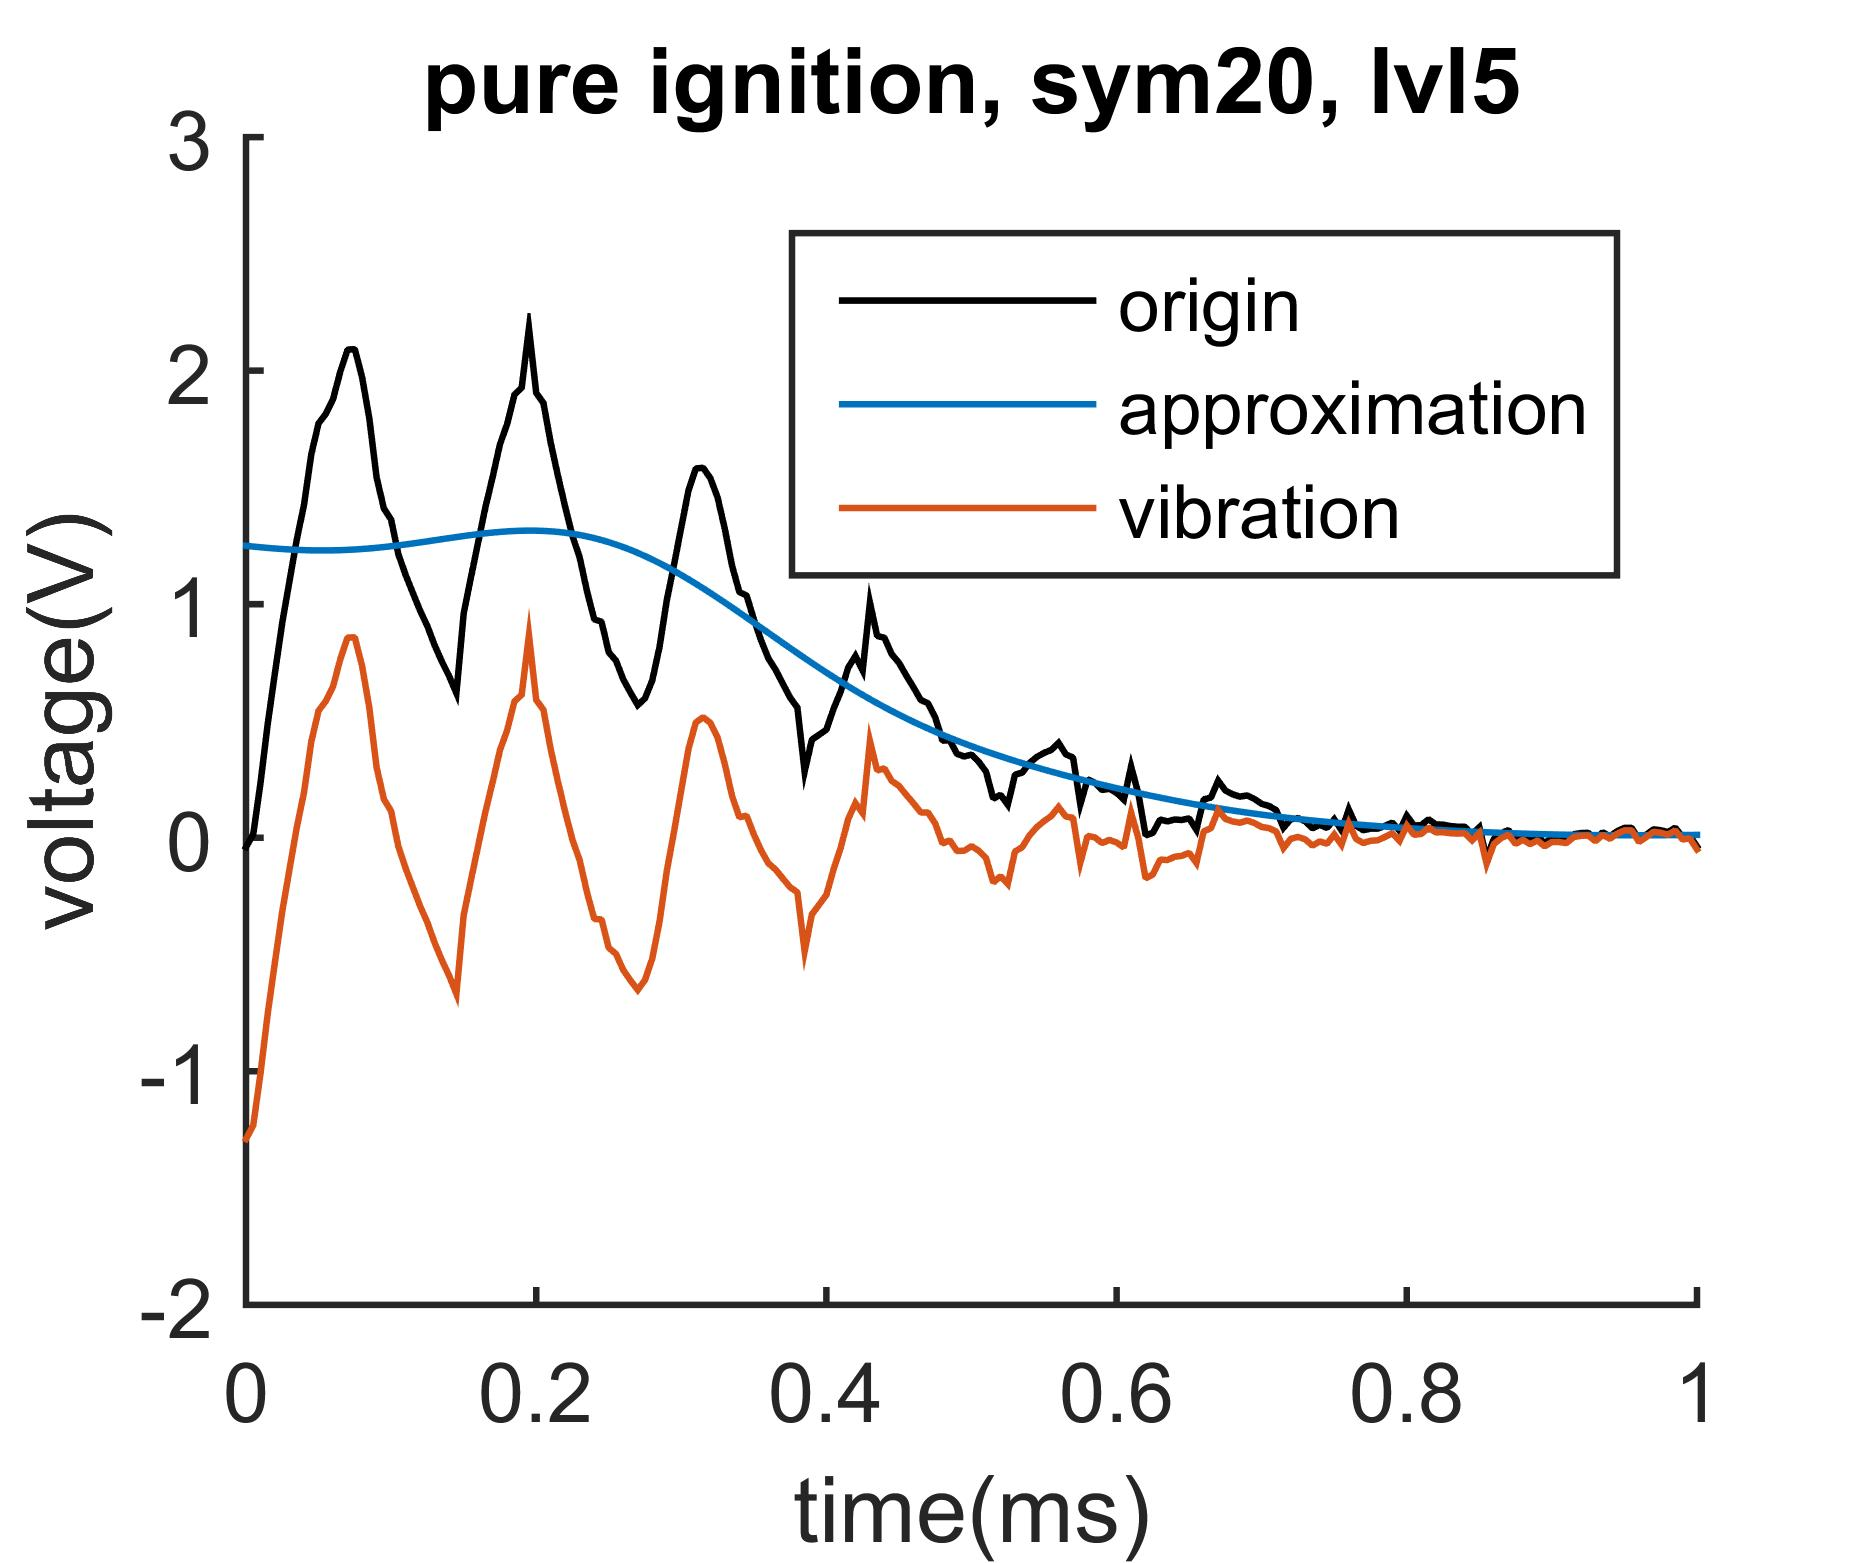
\includegraphics[width=0.3\textwidth]{thesis_figure/ion_chapter/sym20_lvl5}&
		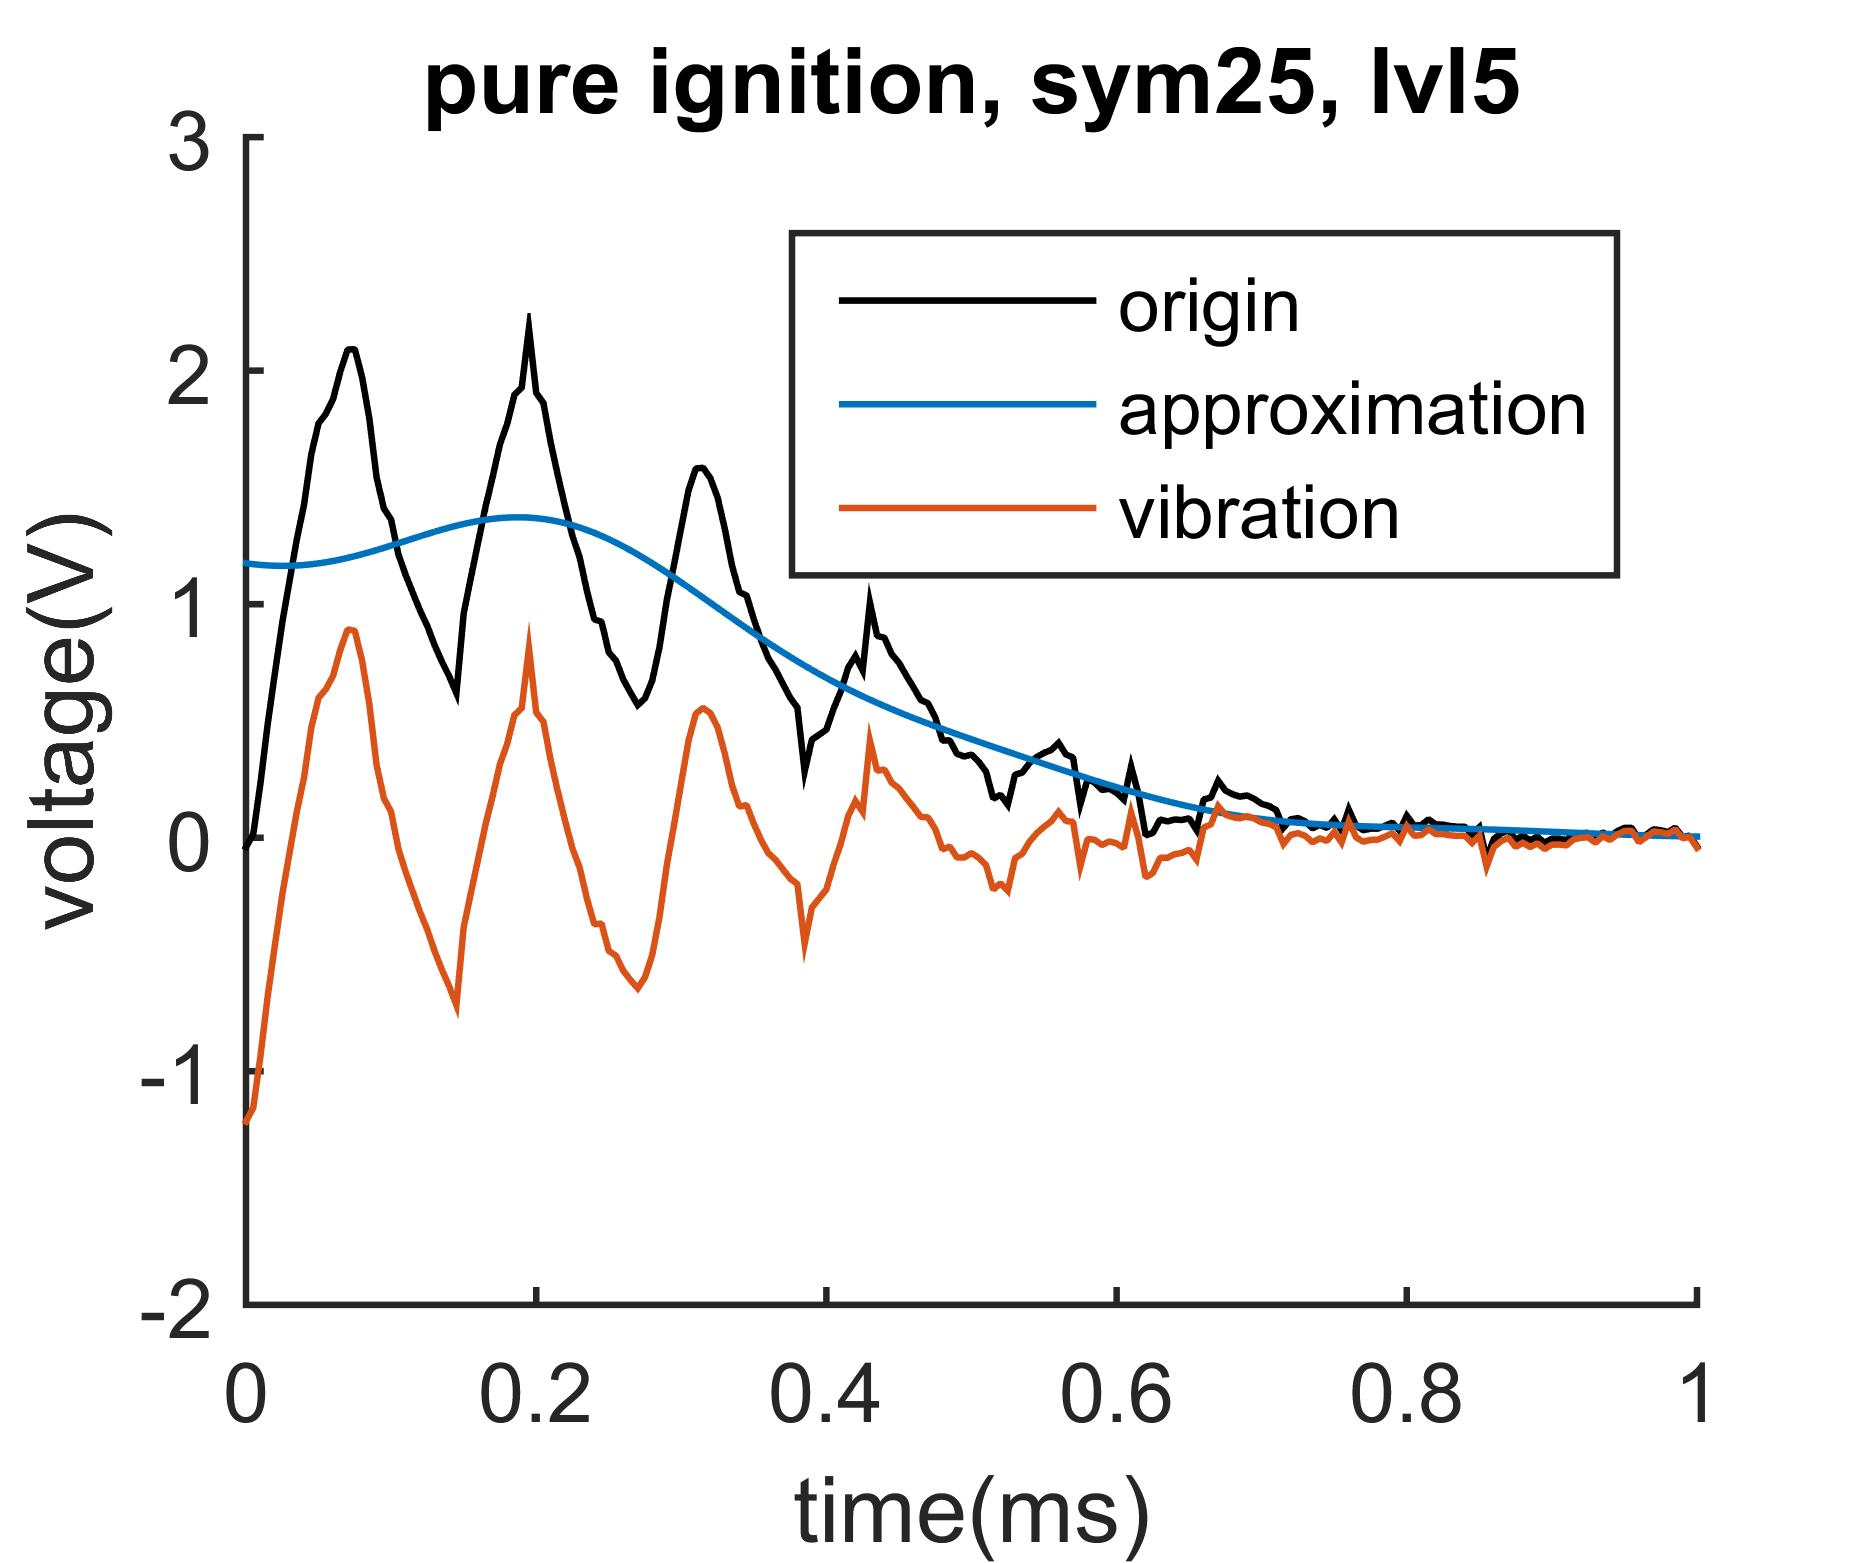
\includegraphics[width=0.3\textwidth]{thesis_figure/ion_chapter/sym25_lvl5}&
		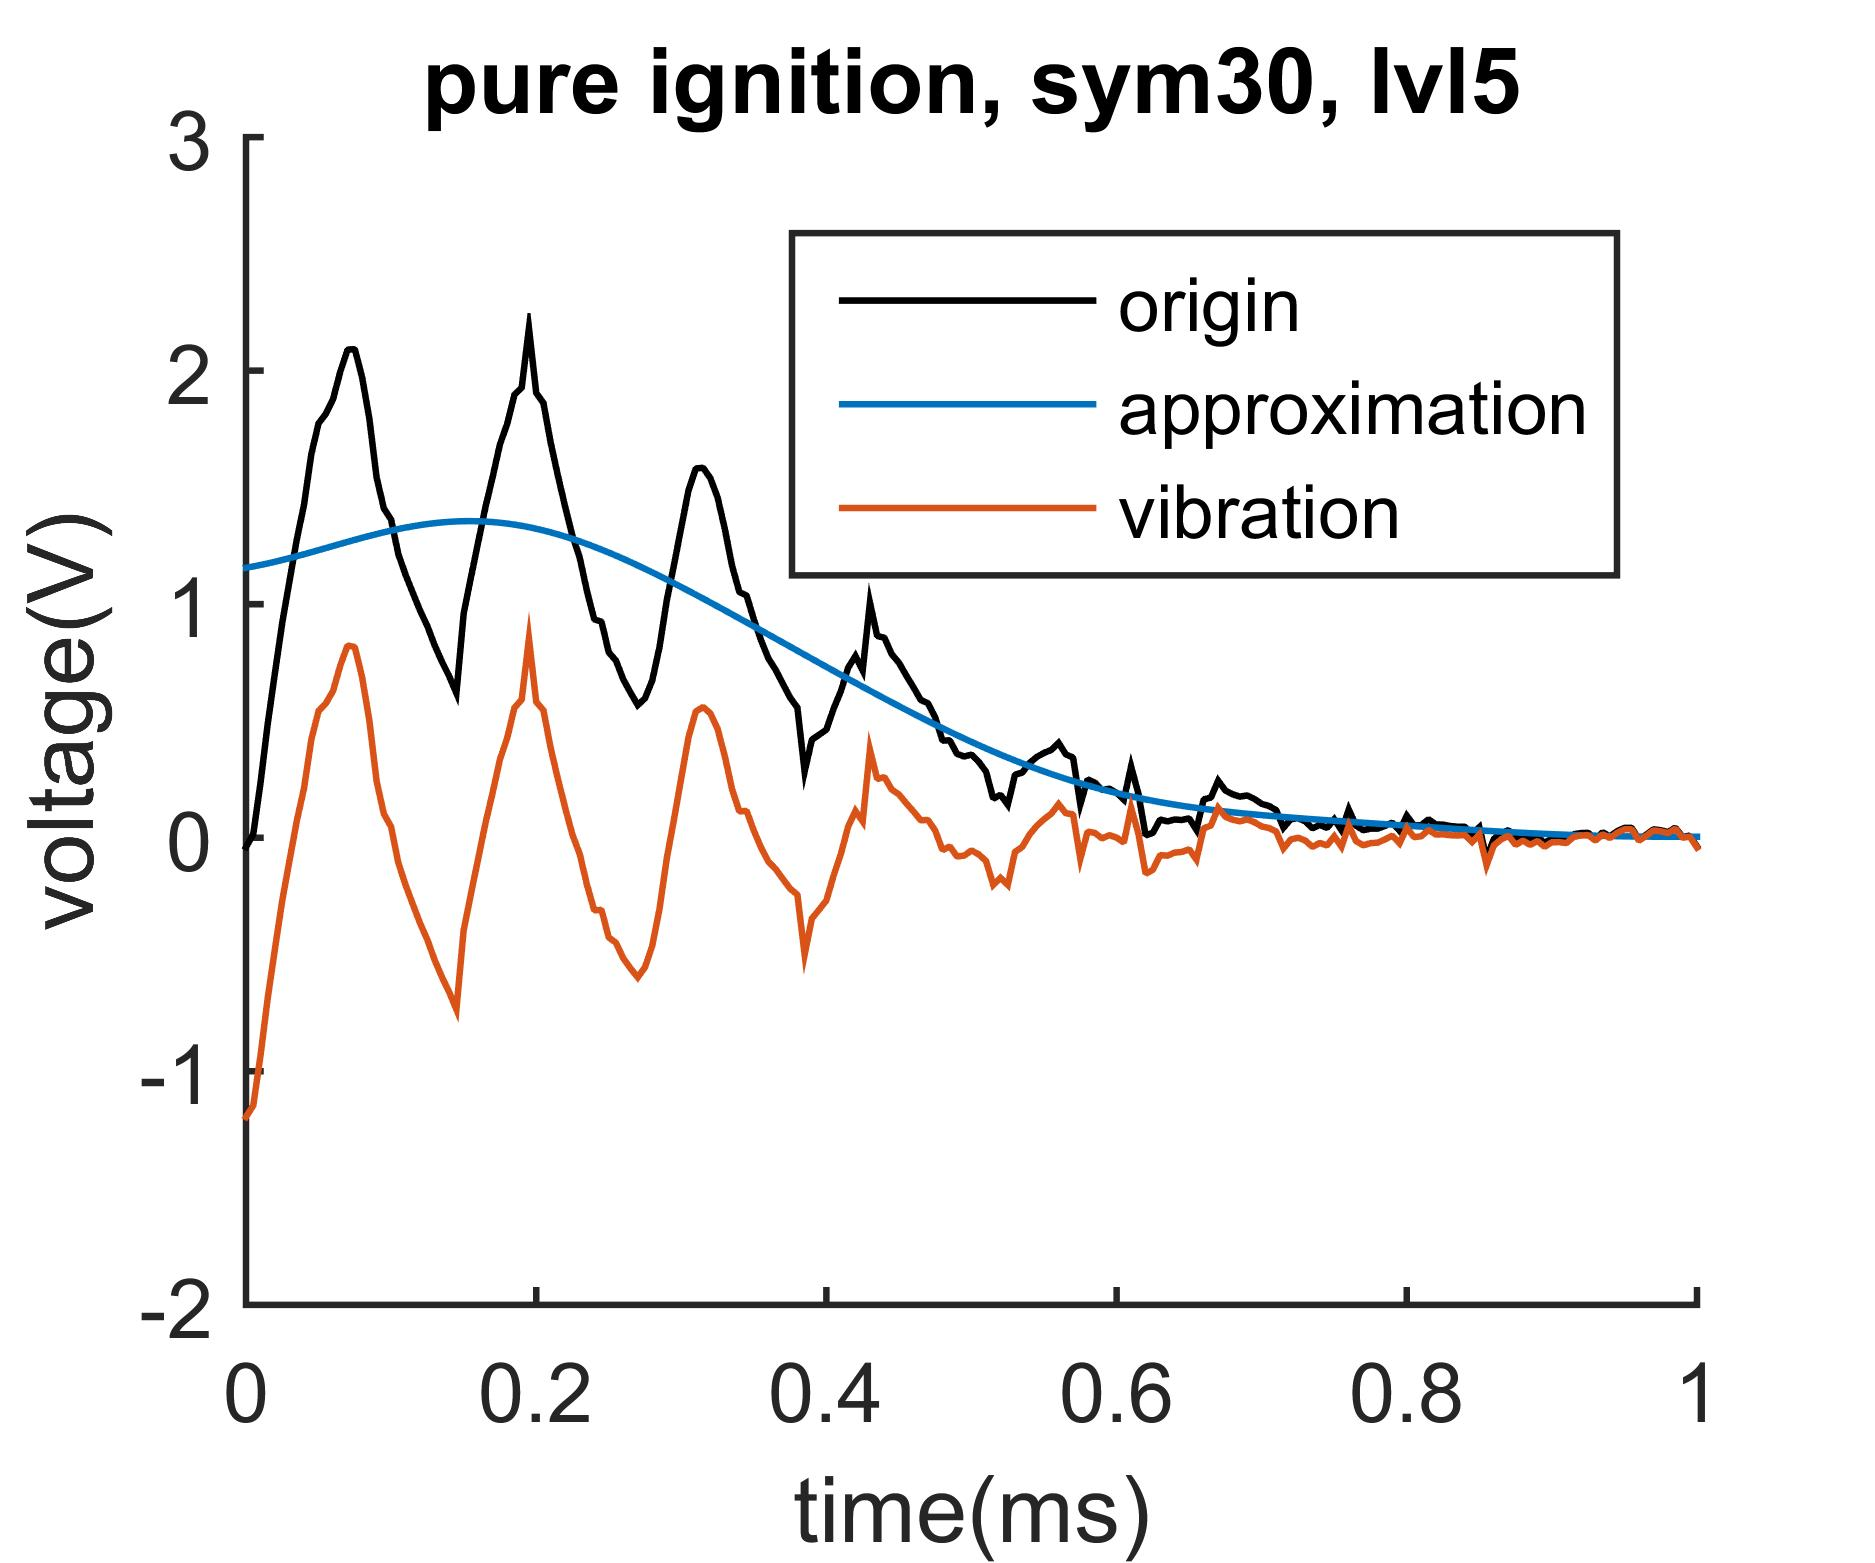
\includegraphics[width=0.3\textwidth]{thesis_figure/ion_chapter/sym30_lvl5}
	\end{tabular}
	\caption{\label{fig:symvar}不同阶数下的sym小波第五层分解}
\end{figure}
从图\ref{fig:symvar}中可以看到当阶数增加到20以后,小波分析第五层分解的结果已经基本不变了,而且随着阶数的增加,sym小波分解的时间增加很快。则取sym20作为sym小波分解的小波函数。
\subsection{四种小波对去除点火干扰分析的比较}
去除点火干扰的方法为用同一个小波基函数对离子电流信号和纯点火干扰信号进行分析,然后两者做差值得出理想的离子电流信号。
\begin{figure}[!ht]
	\centering
	\begin{tabular}{ccc}
		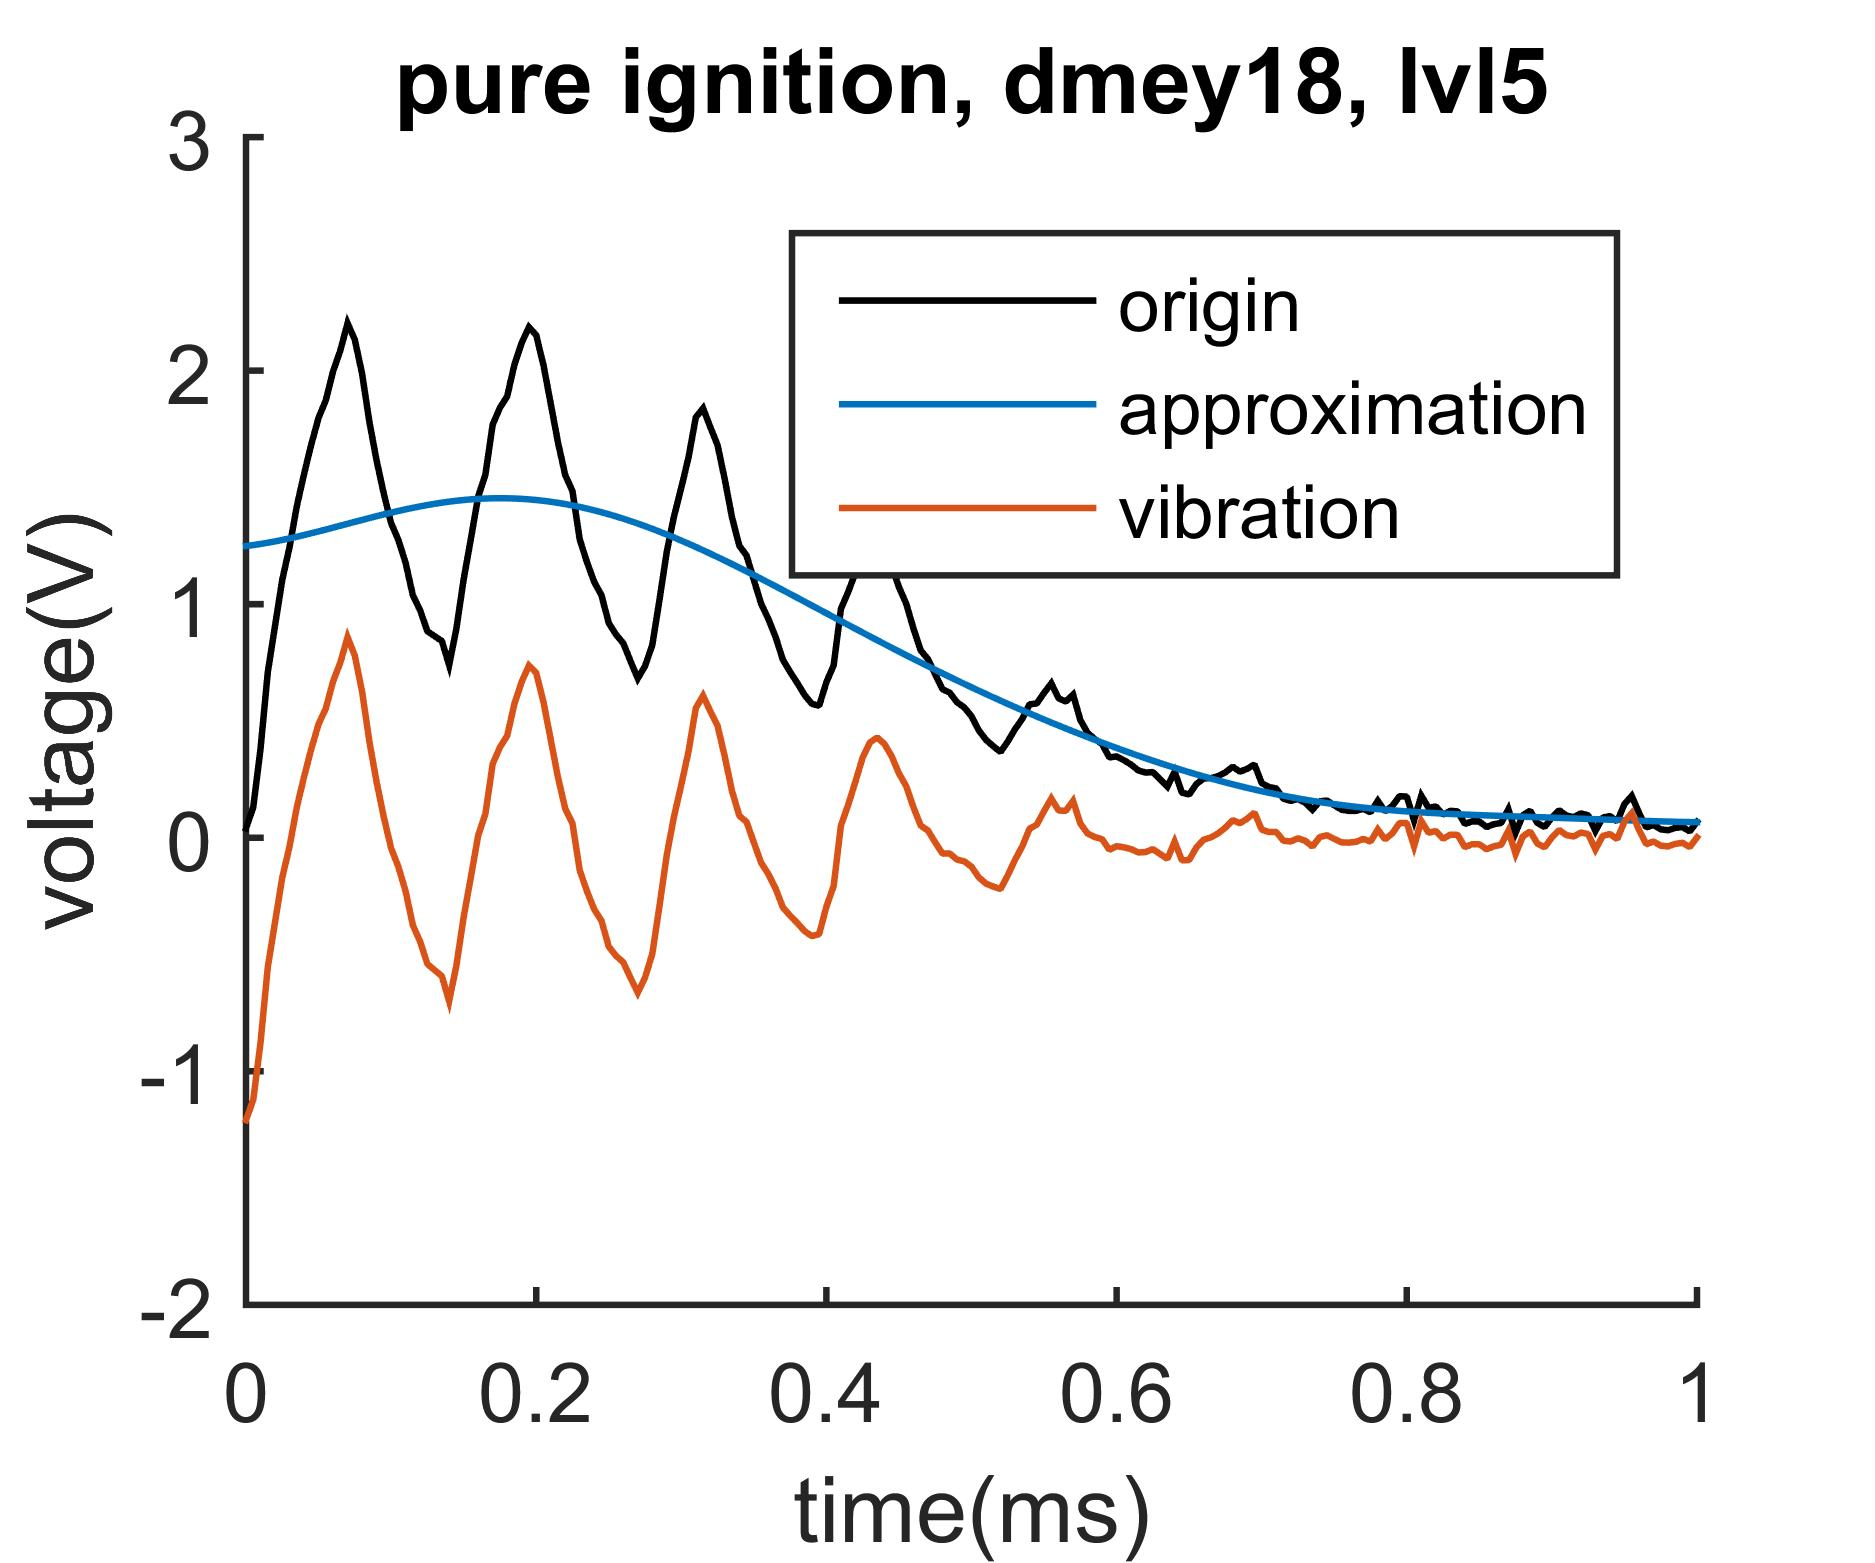
\includegraphics[width=0.4\textwidth]{thesis_figure/ion_chapter/dmey_wafig_pureign}&
		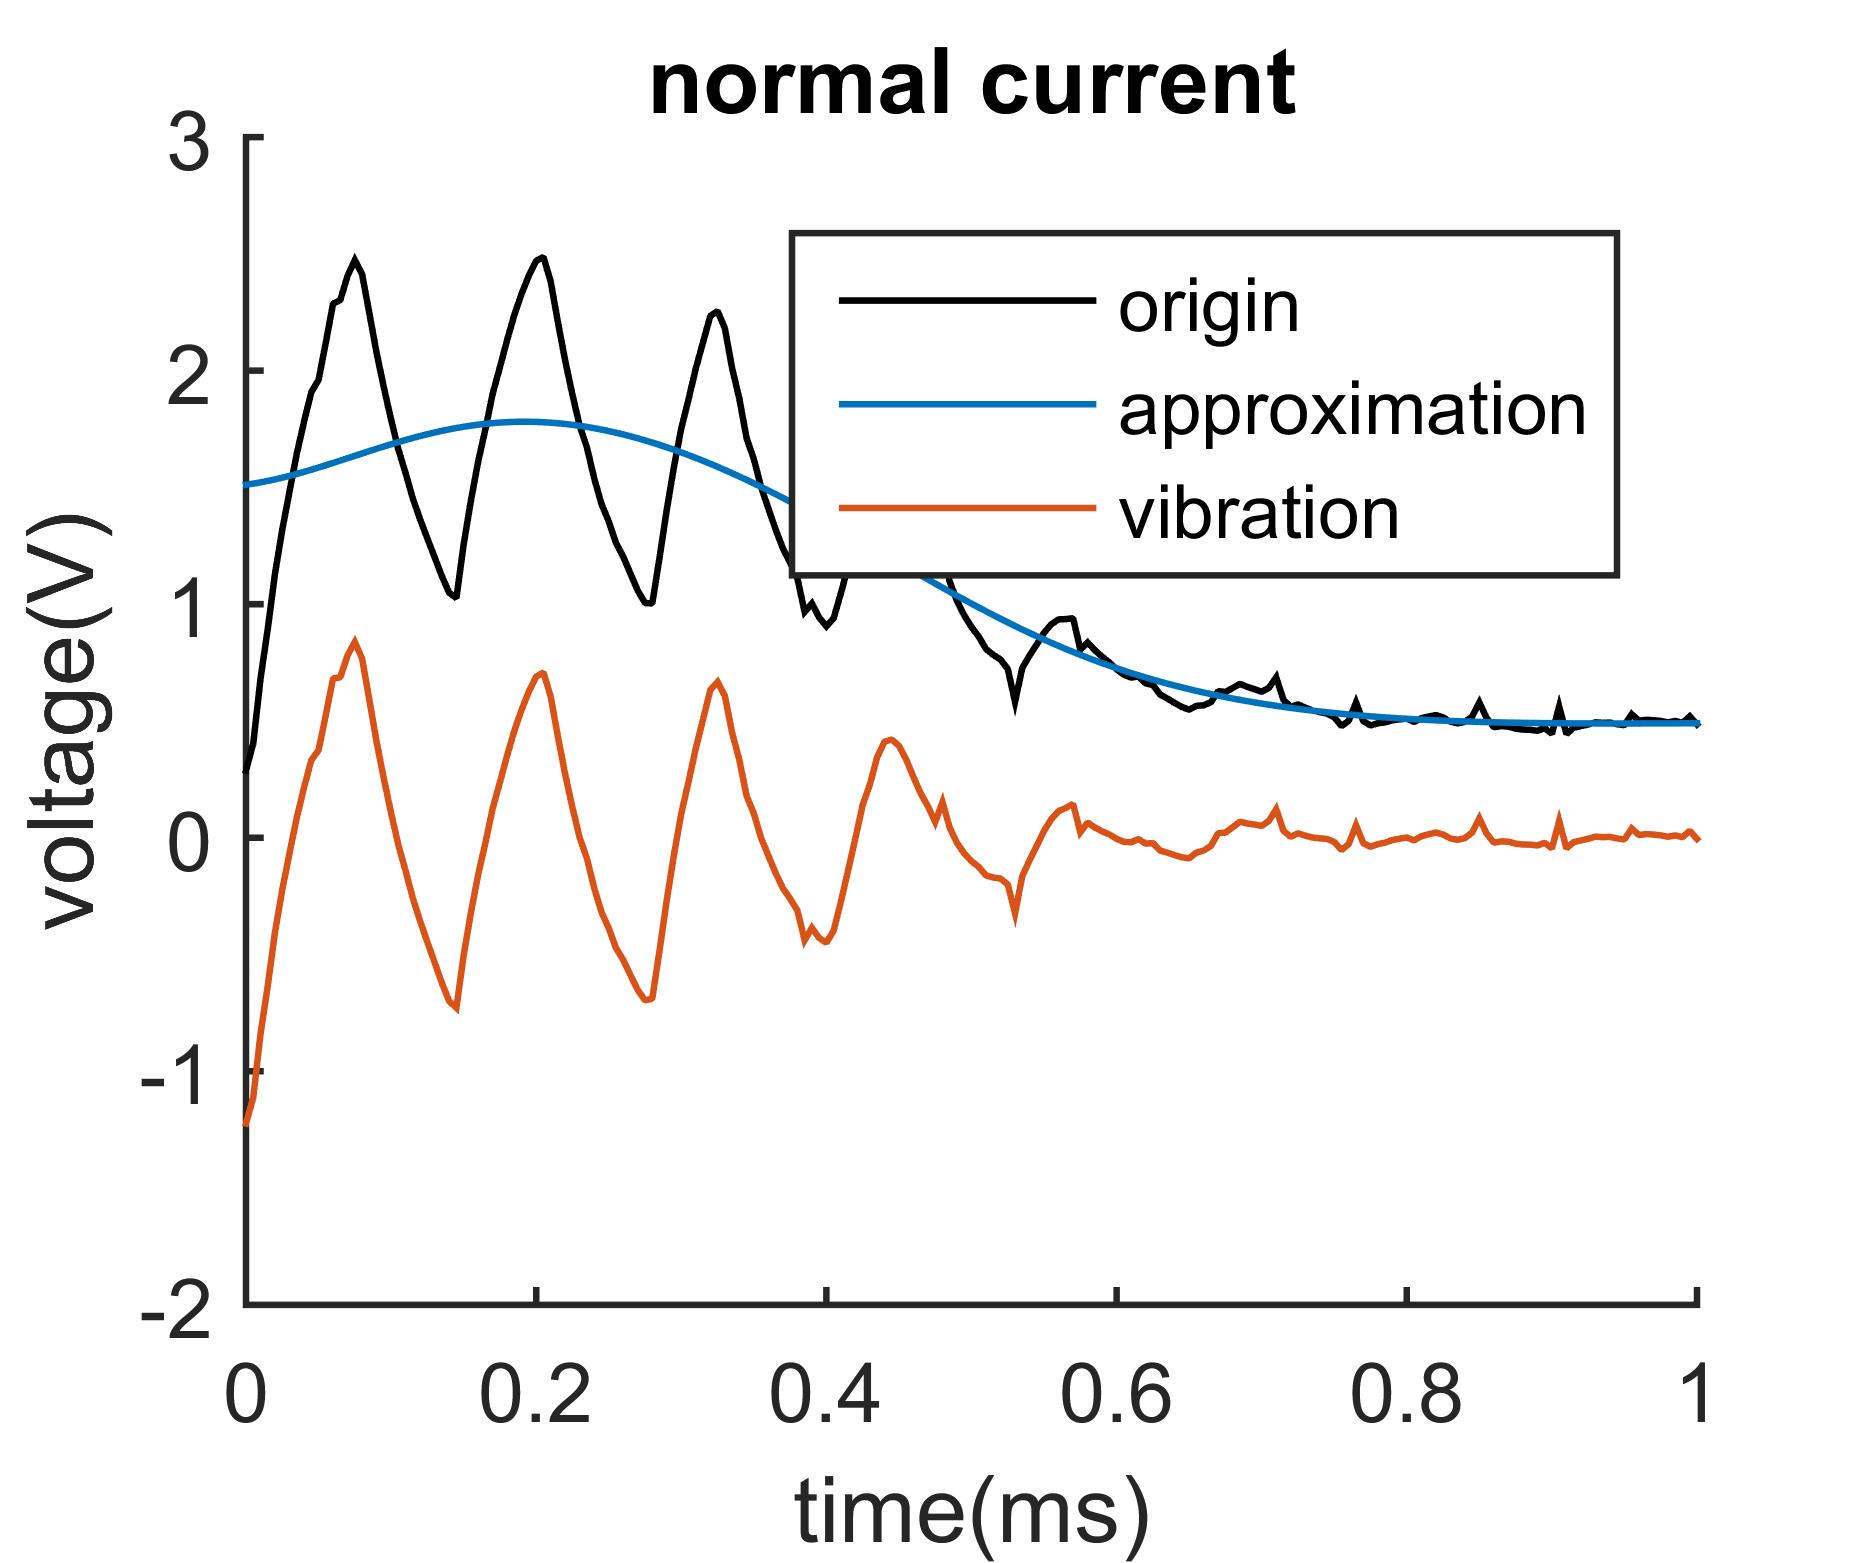
\includegraphics[width=0.4\textwidth]{thesis_figure/ion_chapter/dmey_icfig_norm}\\
		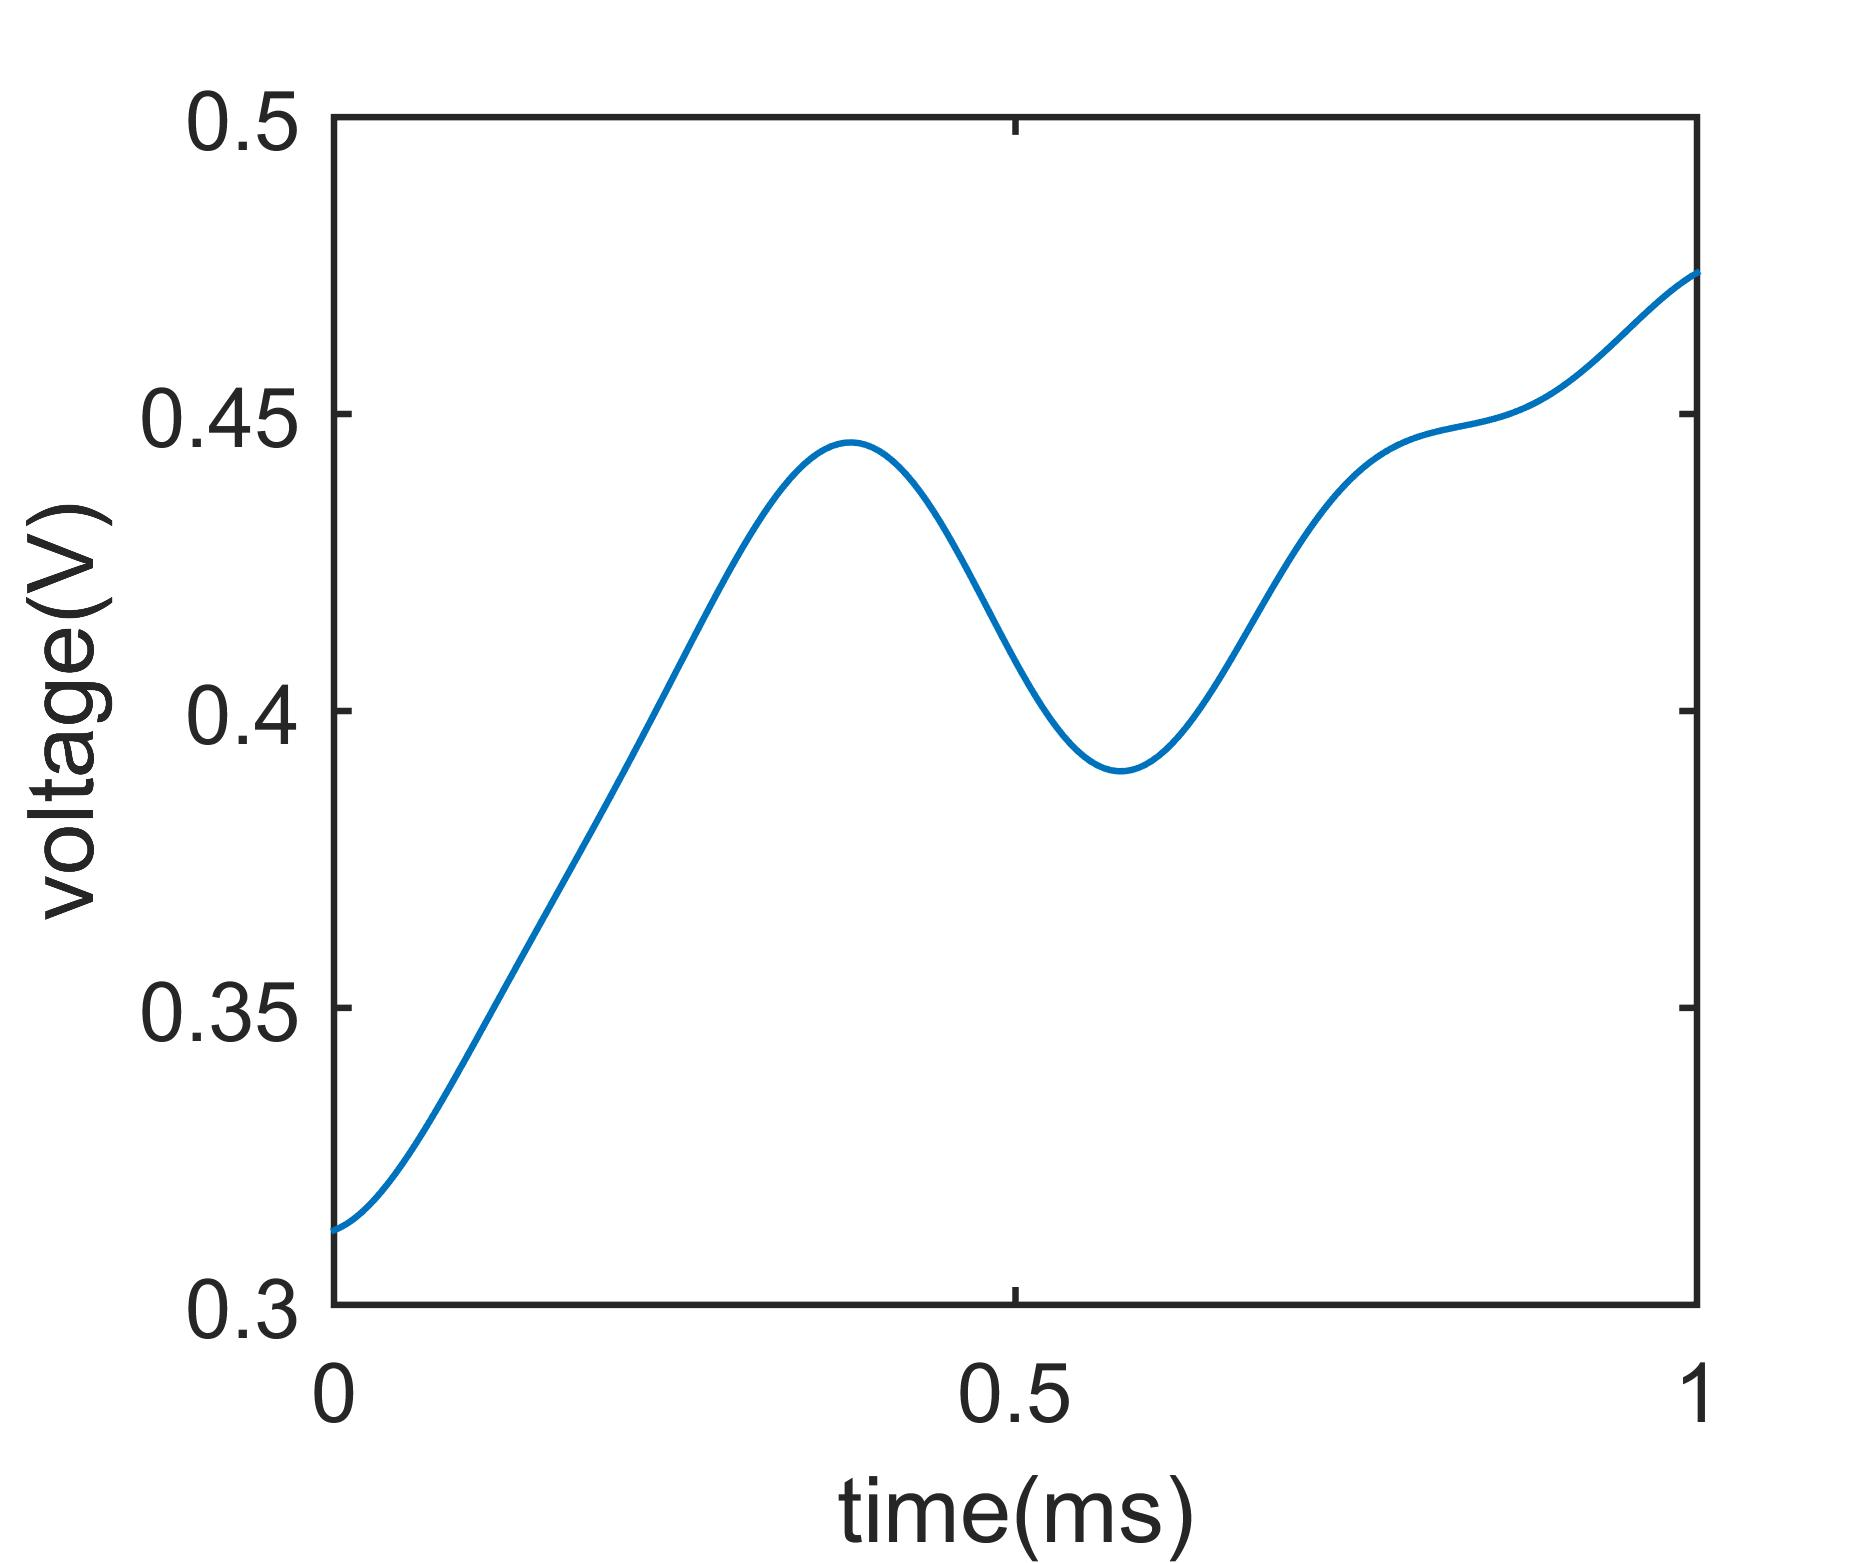
\includegraphics[width=0.4\textwidth]{thesis_figure/ion_chapter/dmey_diffSign}&
		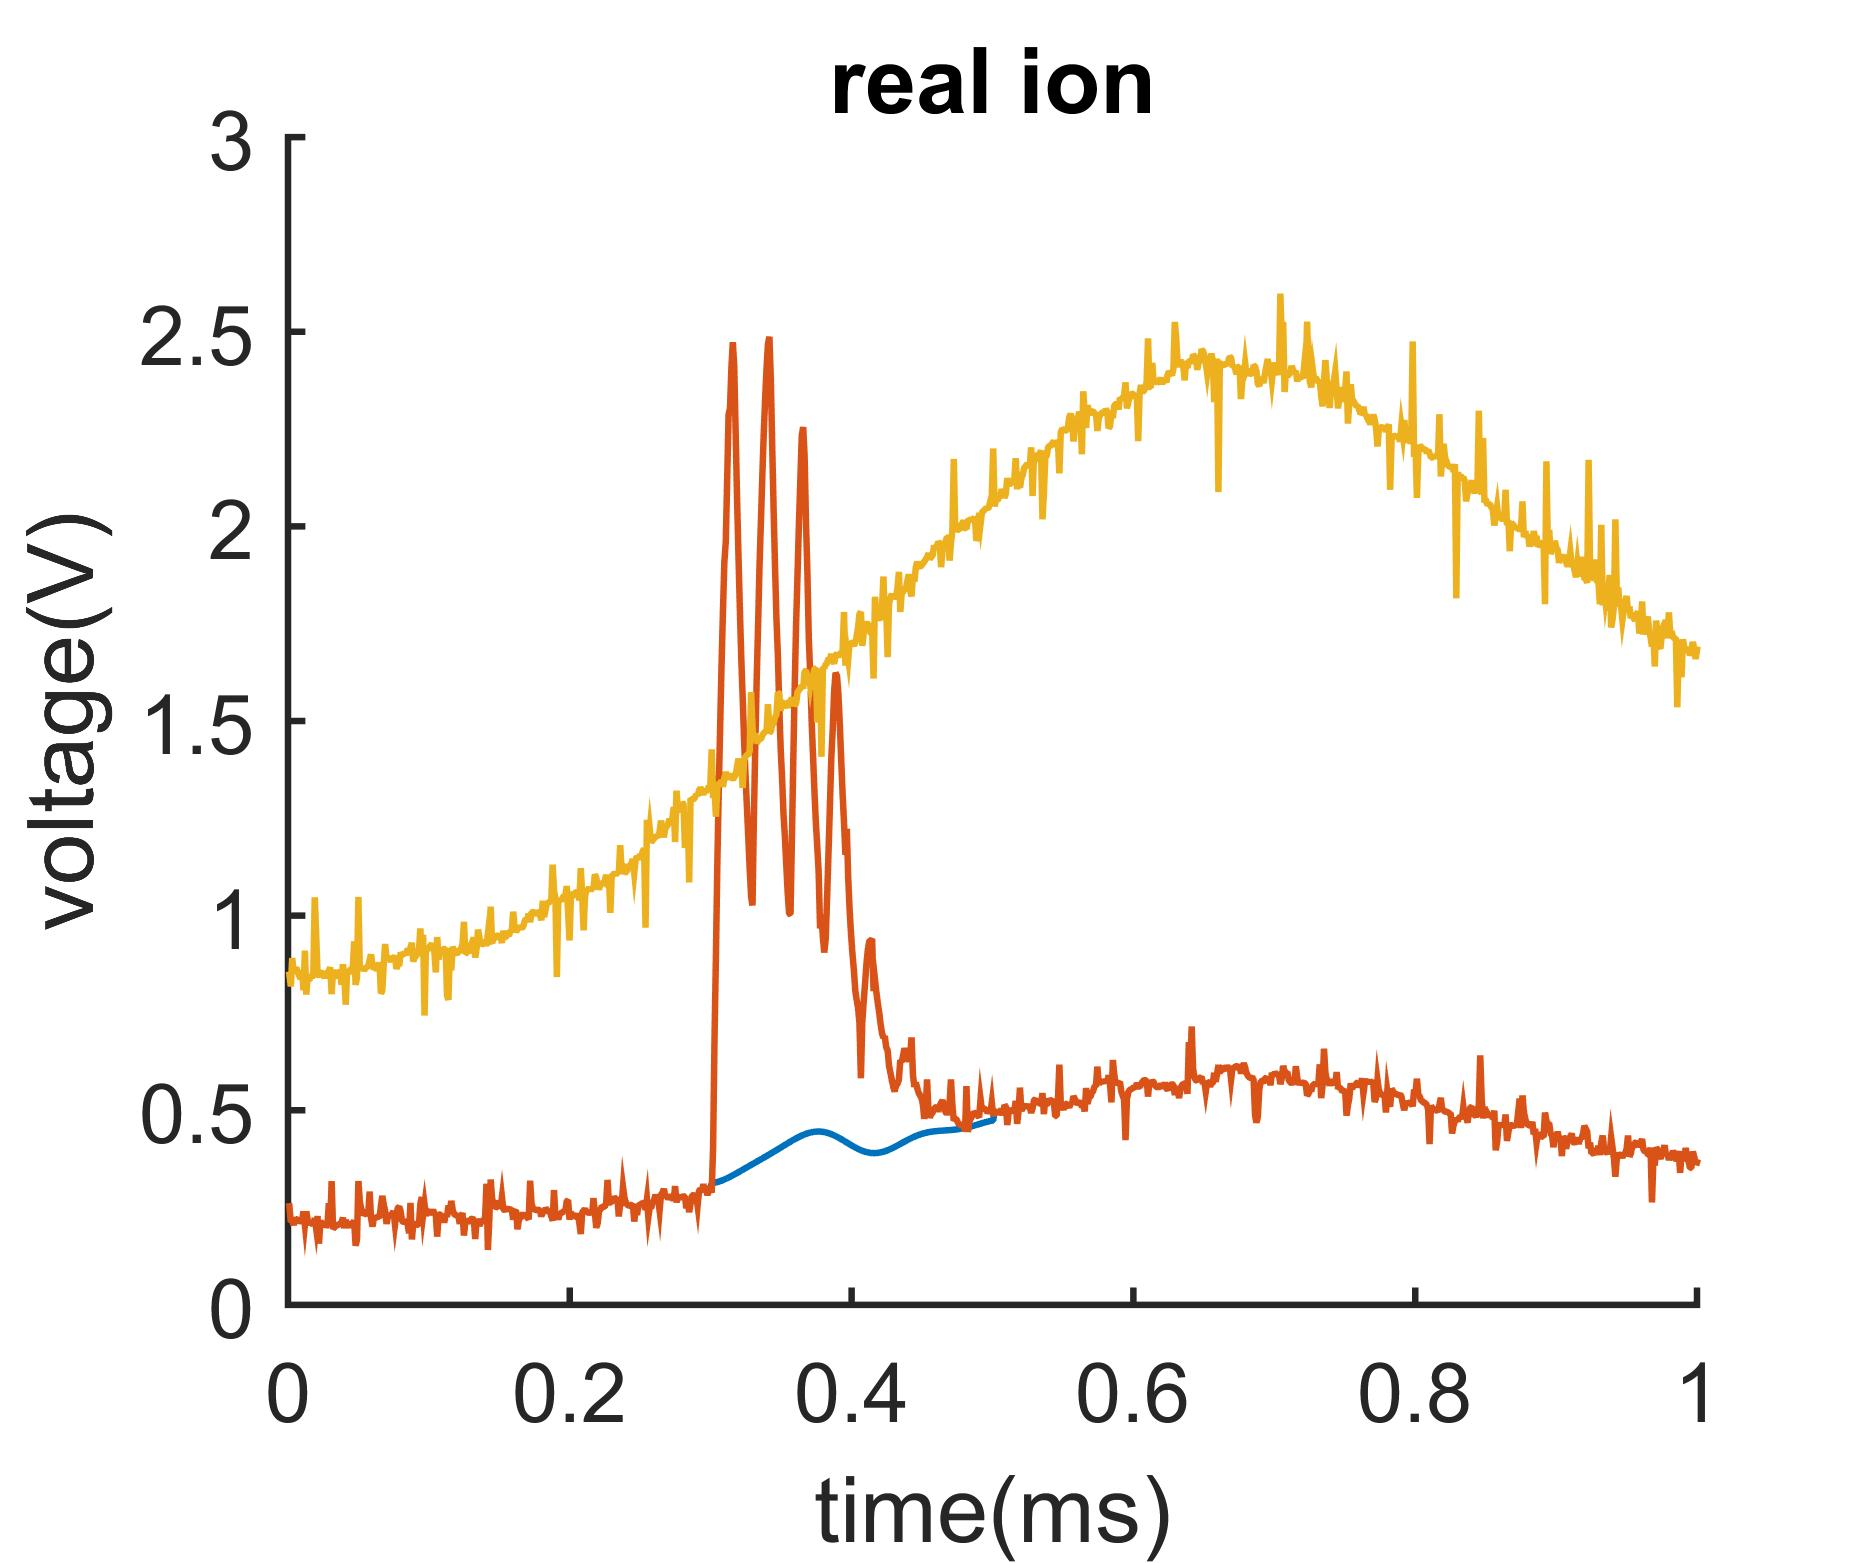
\includegraphics[width=0.4\textwidth]{thesis_figure/ion_chapter/dmey_realIonFig}
	\end{tabular}
	\caption{\label{fig:dmey_realIon}dmey小波分解的真实离子电流信号}
\end{figure}
\par 如图\ref{fig:dmey_realIon}所示的用dmey小波基函数进行小波分析得到的纯点火干扰、离子电流的分解、真实离子电流以及原信号和提取信号比较图。此时的工况为$1000r/min$、40\%负荷,在
此工况下热电离产生的波峰不会被点火干扰淹没。从图中可以看到提取信号可以很好的和原离子电流的其他信号部分进行衔接。从左下角的差值信号中可以看到,该信号存在一个凸起的小峰,此峰即是火焰前锋期造成的离子电流峰,
是火焰锋面从电极一端向另一端扩散过程中化学电离产生的离子电流。
\begin{figure}[!ht]
	\centering
	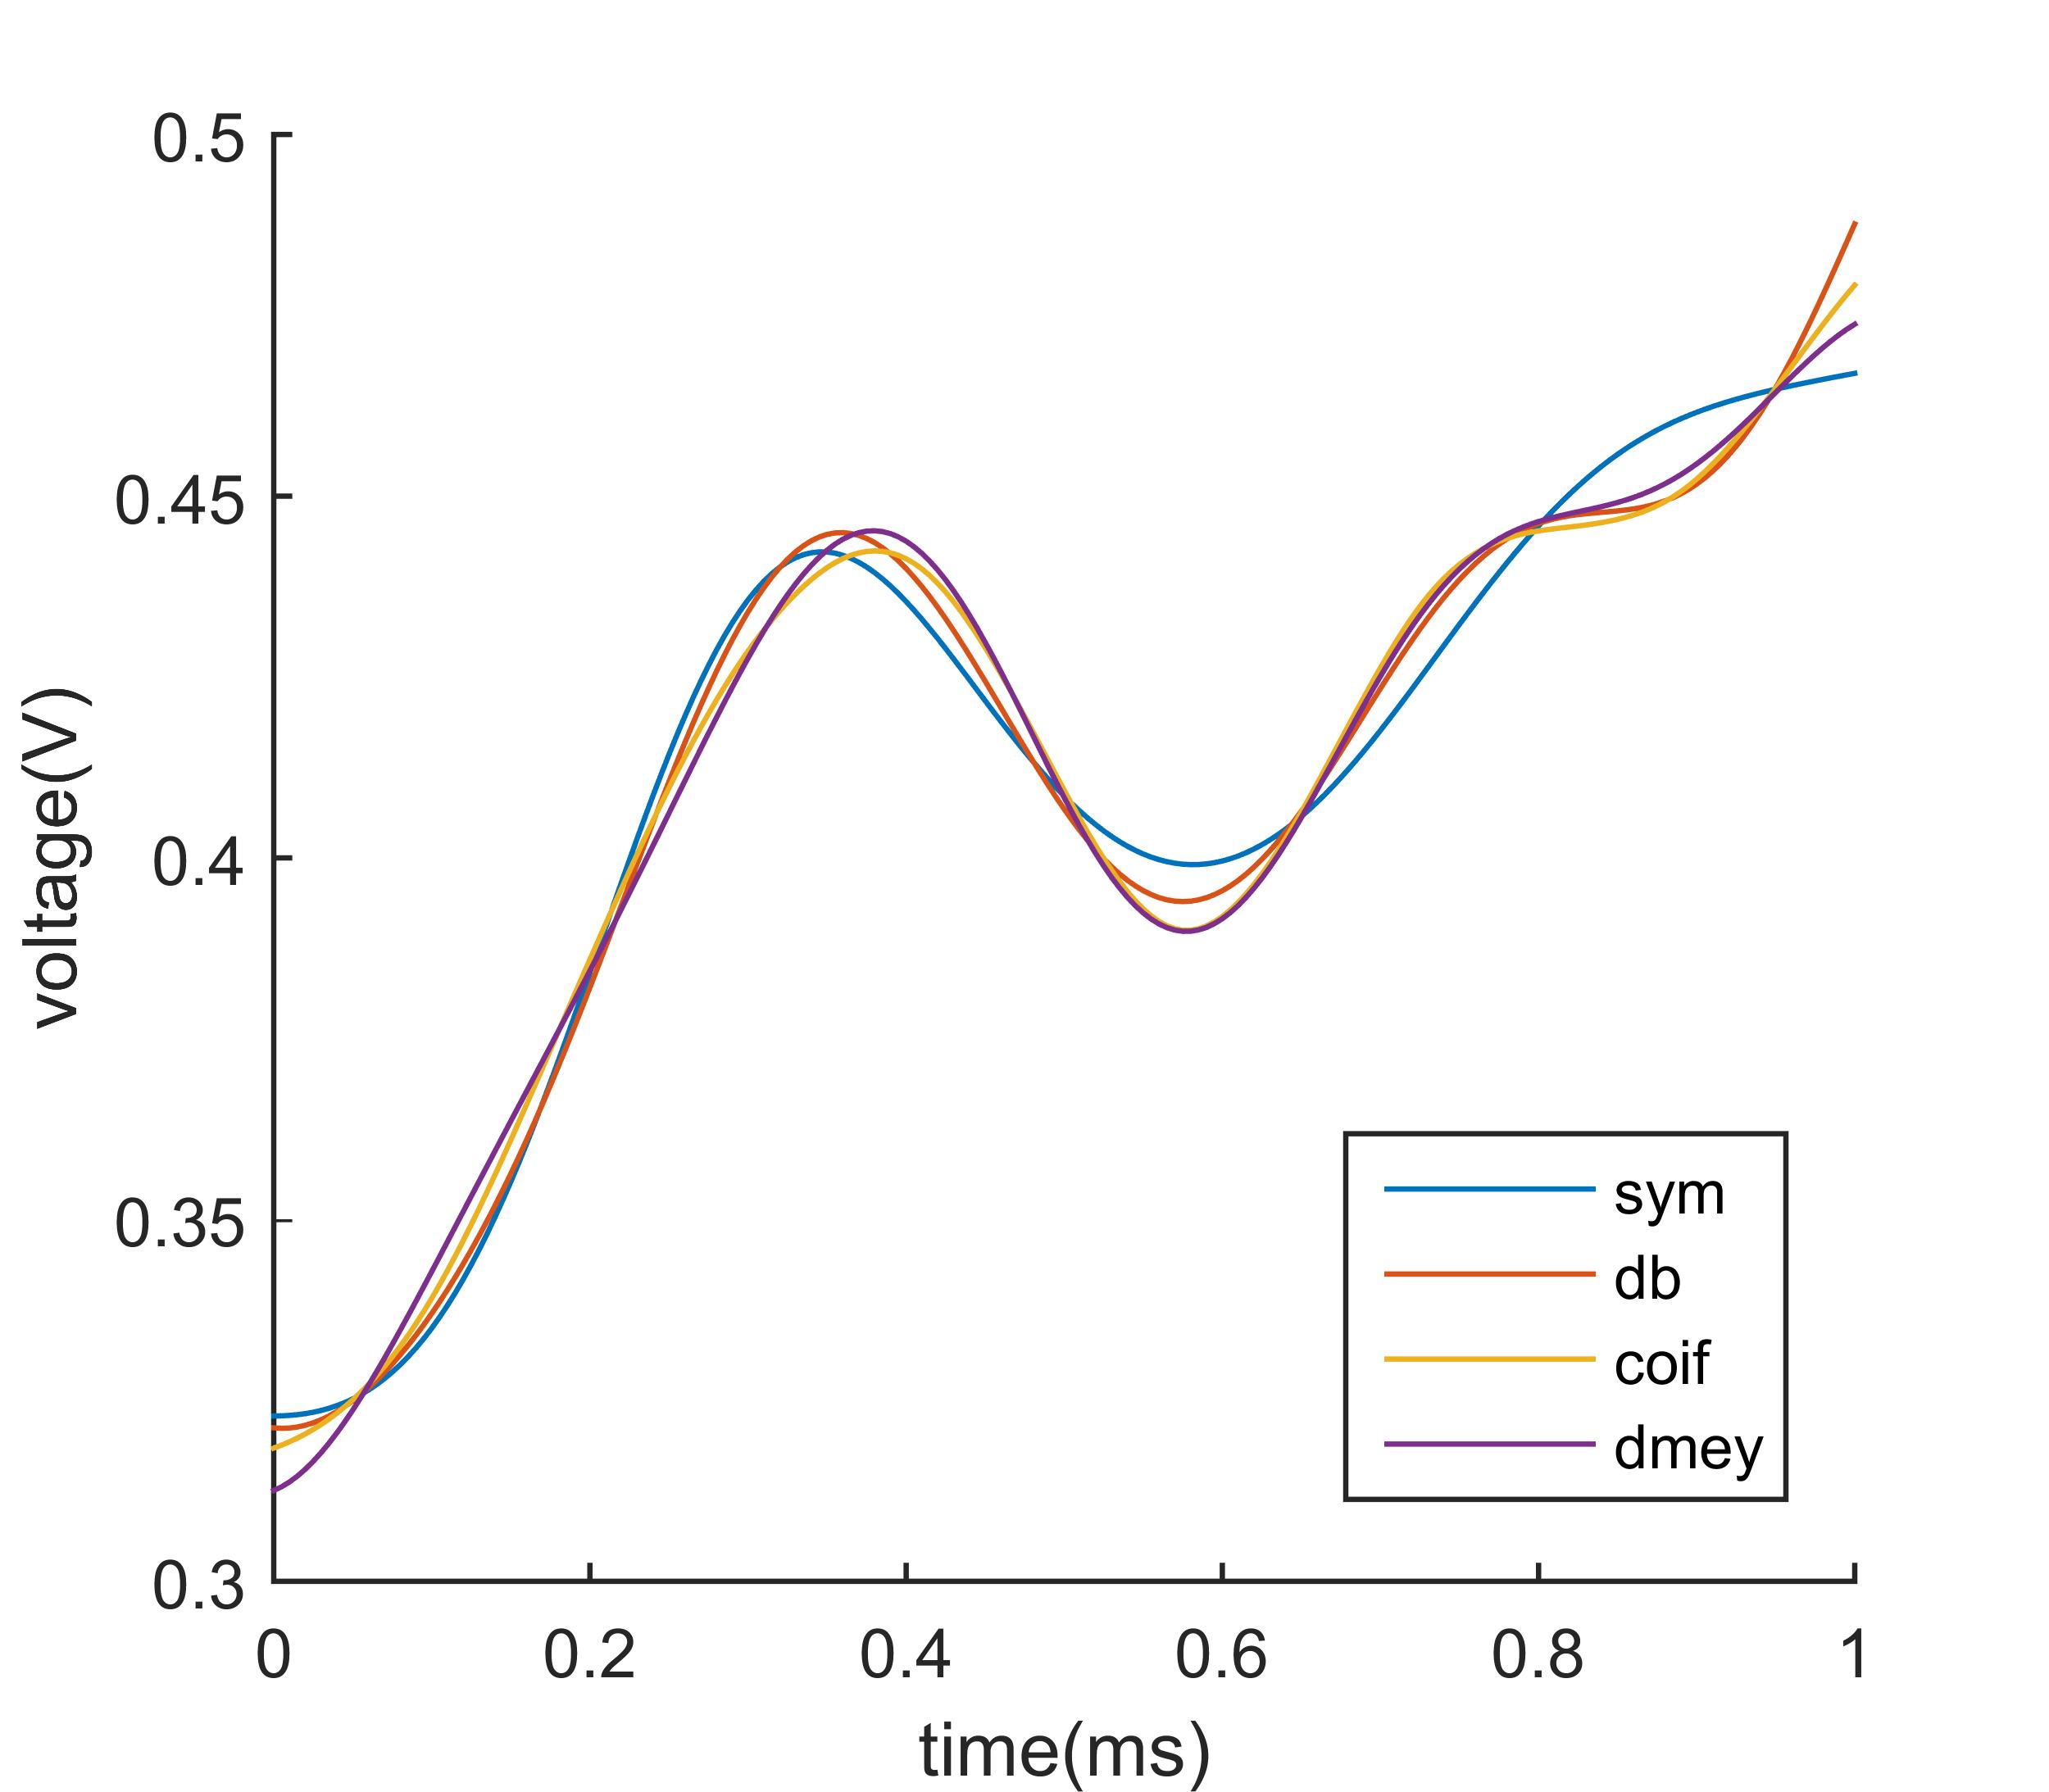
\includegraphics[width=0.5\textwidth]{thesis_figure/ion_chapter/diff_wv_comp}
	\caption{\label{fig:diff_wv_comp}四种小波对真实离子电流进行去干扰处理}
\end{figure}
\par 下图\ref{fig:diff_wv_comp}所示是四种小波对真实离子电流进行处理后的信号比较。从图中可以看到曲线的尖锐程度依次为$dmey>coif>db>sym$,但是差异不大,
都能够明显的显示出火焰前锋期的形状。\par 从相位角度来衡量,四种小波基函数分析结果在关键点的相位上是一样的,能够确定火焰前锋期的开始和结束相位。在曲线的尾段有不同的曲线效果,
这是不同的小波基函数分析结果的最大不同。
\section{高斯曲线拟合估计离子电流特征参数}
\subsection{高斯曲线拟合方法介绍}
来自马里兰大学的T. C. O'Haver给出了曲线拟合的方法\cite{tco_gs}能够有效的对数据进行拟合。根据拟合公式\ref{eqn:interp1}和\ref{eqn:interp2}可以知道,我们可以用两个高斯
函数来对小波分析处理后的离子电流信号曲线进行拟合,从而得到离子电流的关键特征参数。采集到的离子电流曲线有很多杂乱信号,而且整个信号也有部分波动,有较多的峰值。只有通过函数拟合的方
式,才能够较好的获得离子电流特征参数。
\par 拟合方法优劣的评判标准主要是误差分析。
\subsection{双高斯曲线拟合}
给定在$1000r/min$、40\%负荷时的经过小波分析去除干扰的离子电流,经过双高斯曲线拟合方法得到如图所示的曲线。